% !Mode:: "TeX:UTF-8"
%!TEX program  = xelatex

%\documentclass{cumcmthesis}
\documentclass[withoutpreface,bwprint]{cumcmthesis} %去掉封面与编号页

%\usepackage{subfigure}	%用于排版多张图片
\usepackage{float}	%用于排版图片位置
\bibliographystyle{plain}	%引用样式,参考文献
%\usepackage{hyperref}

\usepackage{caption}
\usepackage{graphicx}


\usepackage{subcaption}

\usepackage{enumitem}
\usepackage{graphicx}

\usepackage{url}
\title{基于整数规划和蒙特卡洛模拟的最优生产决策研究}

\begin{document}

\maketitle
\begin{abstract}

在复杂的生产实践中,企业需要一套行之有效的决策方案,使其实现收益最大化。本文建立了基于整数规划和蒙特卡洛模拟的利润最大化模型,并在面对多工序、多零件时引入分段检测机制进行改进,为企业提供了不同生产场景中的具体决策方案。

\textbf{对于问题1},为了设计检测次数尽可能少的抽样检测方案,建立了基于\textbf{假设检验}的\textbf{抽样检测模型}。首先,建立原假设与备择假设,来推断零配件次品率是否超过标称值。然后,利用中心极限定理,将二项分布的样本数据标准化为正态分布,计算出对应的检验统计量。接着,确定在不同置信水平下的置信区间,并得出最小抽样数量与预期次品率的关系式,由此来计算最小抽样数量。最后,给出具体抽样检测方案:针对情形(1),选定预期次品率为\textbf{15\%},则至少抽取并检测\textbf{98}个样本;针对情形(2),选定预期次品率为\textbf{6\%},则抽取并检测\textbf{93}个样本。

\textbf{对于问题2},为了在多种不同的生产情况下为企业提供具有针对性的决策方案,建立了基于\textbf{整数规划}和\textbf{蒙特卡洛模拟}的\textbf{利润最大化模型}。首先,设置模型的初始参数,并针对各个阶段设定决策变量。然后,选定利润最大化为优化目标,并建立目标函数,计算从零配件检测到不合格品调换等各个生产阶段的总成本以及成品的总销售额,得出最终利润。接着,将不同阶段的决策变量代入目标函数与约束条件中,并借助Python实现蒙特卡洛模拟,得出相应情况下最大利润与最优决策方案。最后,针对问题2中的6种情况,分别给出决策方案以及决策依据与指标结果,具体结果见表\ref{biao1}。

\textbf{对于问题3},为了应对多道工序、多个零配件这一更复杂的生产场景,建立了基于\textbf{半成品检测分段机制}的\textbf{利润最大化改进模型}。首先,基于问题2中得到结果以及题目给定的次品率等数值,做出零配件1、2、3,零配件4、5、6,零配件7、8的检测决策一致的假设。接着,引入半成品检测的分段机制,将来源于\textbf{零配件装配}和\textbf{成品拆解}的半成品分开考虑,简化生产流程。然后,通过\textbf{零配件最大化利用策略},得到由零配件到成品的完整流程,结合半成品检测分段机制以及数学公式推导,求解各种成本和利润。最后,通过蒙特卡洛模拟,得到最高利润和最优决策方案,其中最高利润为\textbf{75.49元}。

\textbf{对于问题四},为了更新问题2和问题3中零配件、半成品和成品的次品率,选择沿用问题1中的抽样检测方法。首先,基于问题1中的两种情形,设计了抽取\textbf{100个样本}的抽样方案,分别求得对应的次品率为\textbf{15\%}与\textbf{6\%}。然后,对两种情形分别用抽样检测得到的对应次品率替换问题2和问题3中的次品率,并重新完成问题2与问题3的决策过程,得出次品率更新之后的最优决策方案。其中,问题3在95\%置信水平下的最高利润为\textbf{71.15元},在90\%置信水平下的最高利润为\textbf{120.53元}。


\keywords{抽样检测\quad 整数规划\quad 蒙特卡洛模拟\quad 半成品检测分段机制  }

\end{abstract}

%目录
%\tableofcontents

%新的一页
%\newpage

\section{问题重述}

\subsection{问题背景}

近年来,随着全球化进程的深入和国际贸易环境的变化,制造业面临着日益激烈的市场竞争。质量是市场竞争的焦点,信誉是占领市场的先决条件。质量体系是一个企业参与市场竞争的敲门砖,能够反映企业的整体素质和综合竞争实力。\cite{魏富选2010汽车电子零部件企业的产品质量观}然而,由于供应链的复杂性,如何在保证产品质量的同时有效地控制成本,成为了亟待解决难题。

因此,针对零配件的采购、组装与产品生产过程的优化问题,为企业提供一个科学合理的决策支持系统,在保证产品质量的同时,优化生产流程并降低不必要的开支,对于企业在市场中的夺取竞争优势、实现成本和质量的双赢,具有重要意义。

\subsection{问题重述}

某企业需从供应商处采购两种零配件,并装配成电子产品。然而,供应商的零配件存在一定的次品率,不仅影响成品的合格率,还会增加检测成本。此外,即便所有零配件都合格,成品仍可能因装配问题而不合格,从而增加企业的调换损失和拆解费用。因此,企业需要制定一套有效的质量控制策略,来完成对零配件的检验、成品的检测以及不合格产品的处理过程。

试建立数学模型,解决以下问题:

\textbf{问题1:}企业需要决定如何最有效地对供应商提供的两种零配件进行抽样检测,以确保次品率不超过标称值,且检测成本最低。设计一种在检测次数最少的前提下,确定零配件合格与否的方案,并在标称值为10\%时,分别针对在95\%和90\%的置信水平下零配件是否符合标准,制定具体的抽样检测方案。

\textbf{问题2:}在已知两种零配件及成品次品率的情况下,企业需要在是否检测零配件,是否检测成品,是否拆解不合格成品,及如何处理退回的不合格产品等多个环节作出决策。针对表1中企业在生产中可能遇到的六种情况,为各个阶段做出决策,并给出决策依据和指标结果,最终实现在最小化成本和损失的同时,最大化产品质量和客户满意度。

\textbf{问题3:}将问题二中的结论推广到包含多道工序和多个零配件的生产流程中。在已知零配件、半成品和成品的次品率的条件下,依据图1所示的生产工序和组装情况,为表2所示的情况制定生产决策,确保整个生产过程中产品的高质量和低成本,并给出决策依据和结果。

\textbf{问题4:}假设之前的问题中所有关于次品率的数据都是通过抽样检测获得的,重新考虑问题2和问题3中的生产决策,需要评估新的抽样结果如何影响先前的结论,并基于抽样检测方法更新生产策略。

\section{问题分析}

\subsection{问题1分析}

\textbf{对于问题1},企业需要设计一个合理的抽样检测方案,使得在检测次数最少的前提下,判断零配件的次品率是否超过标称值。题目提供的零配件的标称次品率为10\%,并要求在95\%和90\%的置信水平下分别进行抽样检测,并设计抽样检测方案。对此,建立假设检验模型求解最小抽样数量。首先,建立原假设和备择假设,用来推断零配件的次品率是否超过标称值。接着,选取检验统计量,以样本次品率估计总体次品率,并利用中心极限定理将样本数据标准化为正态分布,计算出对应的检验统计量。然后,通过查找不同置信水平下的临界值,计算出零配件的接收和拒收条件。最后,得出样本次品率和最小抽样数量的关系式,并由此计算出最小抽样数量,确保在给定的置信水平下,能够在样本量最小的情况下判断零配件是否符合要求。

\subsection{问题2分析}

\textbf{对于问题2},题目要求在已知零配件次品率、成品次品率及各环节的成本信息的条件下,优化企业生产过程中多个决策环节,并给出最优的决策方案,旨在实现利润最大化。首先,设置模型的初始参数,并将每个环节的决策设定为决策变量。接下来,建立基于整数规划的利润最大化模型,通过计算从零配件检测到成品拆解等一系列环节的总成本,以及成品的销售额,得到最终利润。最后,通过将不同环节的决策变量代入目标函数和约束条件中,借助Python实现蒙特卡洛模拟,计算出最优的生产策略,以达到在控制成本的同时确保产品质量的目的,最终实现利润最大化并得出具体数值。

\subsection{问题3分析}

\textbf{对于问题3},问题三是对问题二的推广和提升,不仅增加了零配件个数,还增加了工序,产生了半成品这一中间过程,大大增加了决策复杂度。首先,依据问题2得出的结果和实际生活经验,假设零配件1、2、3,零配件4、5、6和零配件7、8做出相同的零配件检测决策。然后,依据零配件最大化利用策略,即当半成品不再生成时才开始由半成品装配成品,来模拟半成品到成品的过程。通过半成品分段检测机制来计算半成品的检测和拆解成本,并计算收益和其他成本,进而得到最终利润。借助Python实现蒙特卡洛模拟,得到最大利润和最优决策方案。

\subsection{问题4分析}

\textbf{对于问题4},它是前三个问题的综合应用。为了更新问题2和问题3中零配件、半成品和成品的次品率,需要沿用问题1中的抽样检测方法。首先,基于问题1中的两个情形,使用其给定的置信水平以及标称值,设计抽取一定样本数量的抽样方案来分别求得对应的次品率。然后,对两种情形分别将对应次品率替换为问题2和问题3中的次品率,并重新完成问题2与问题3,得出次品率更新后的最优决策方案。

综上所述,本文的分析与研究过程如下图所示:
\begin{figure}[htbp]  %h此处,t页顶,b页底,p独立一页,浮动体出现的位置
	\centering  %图表居中
	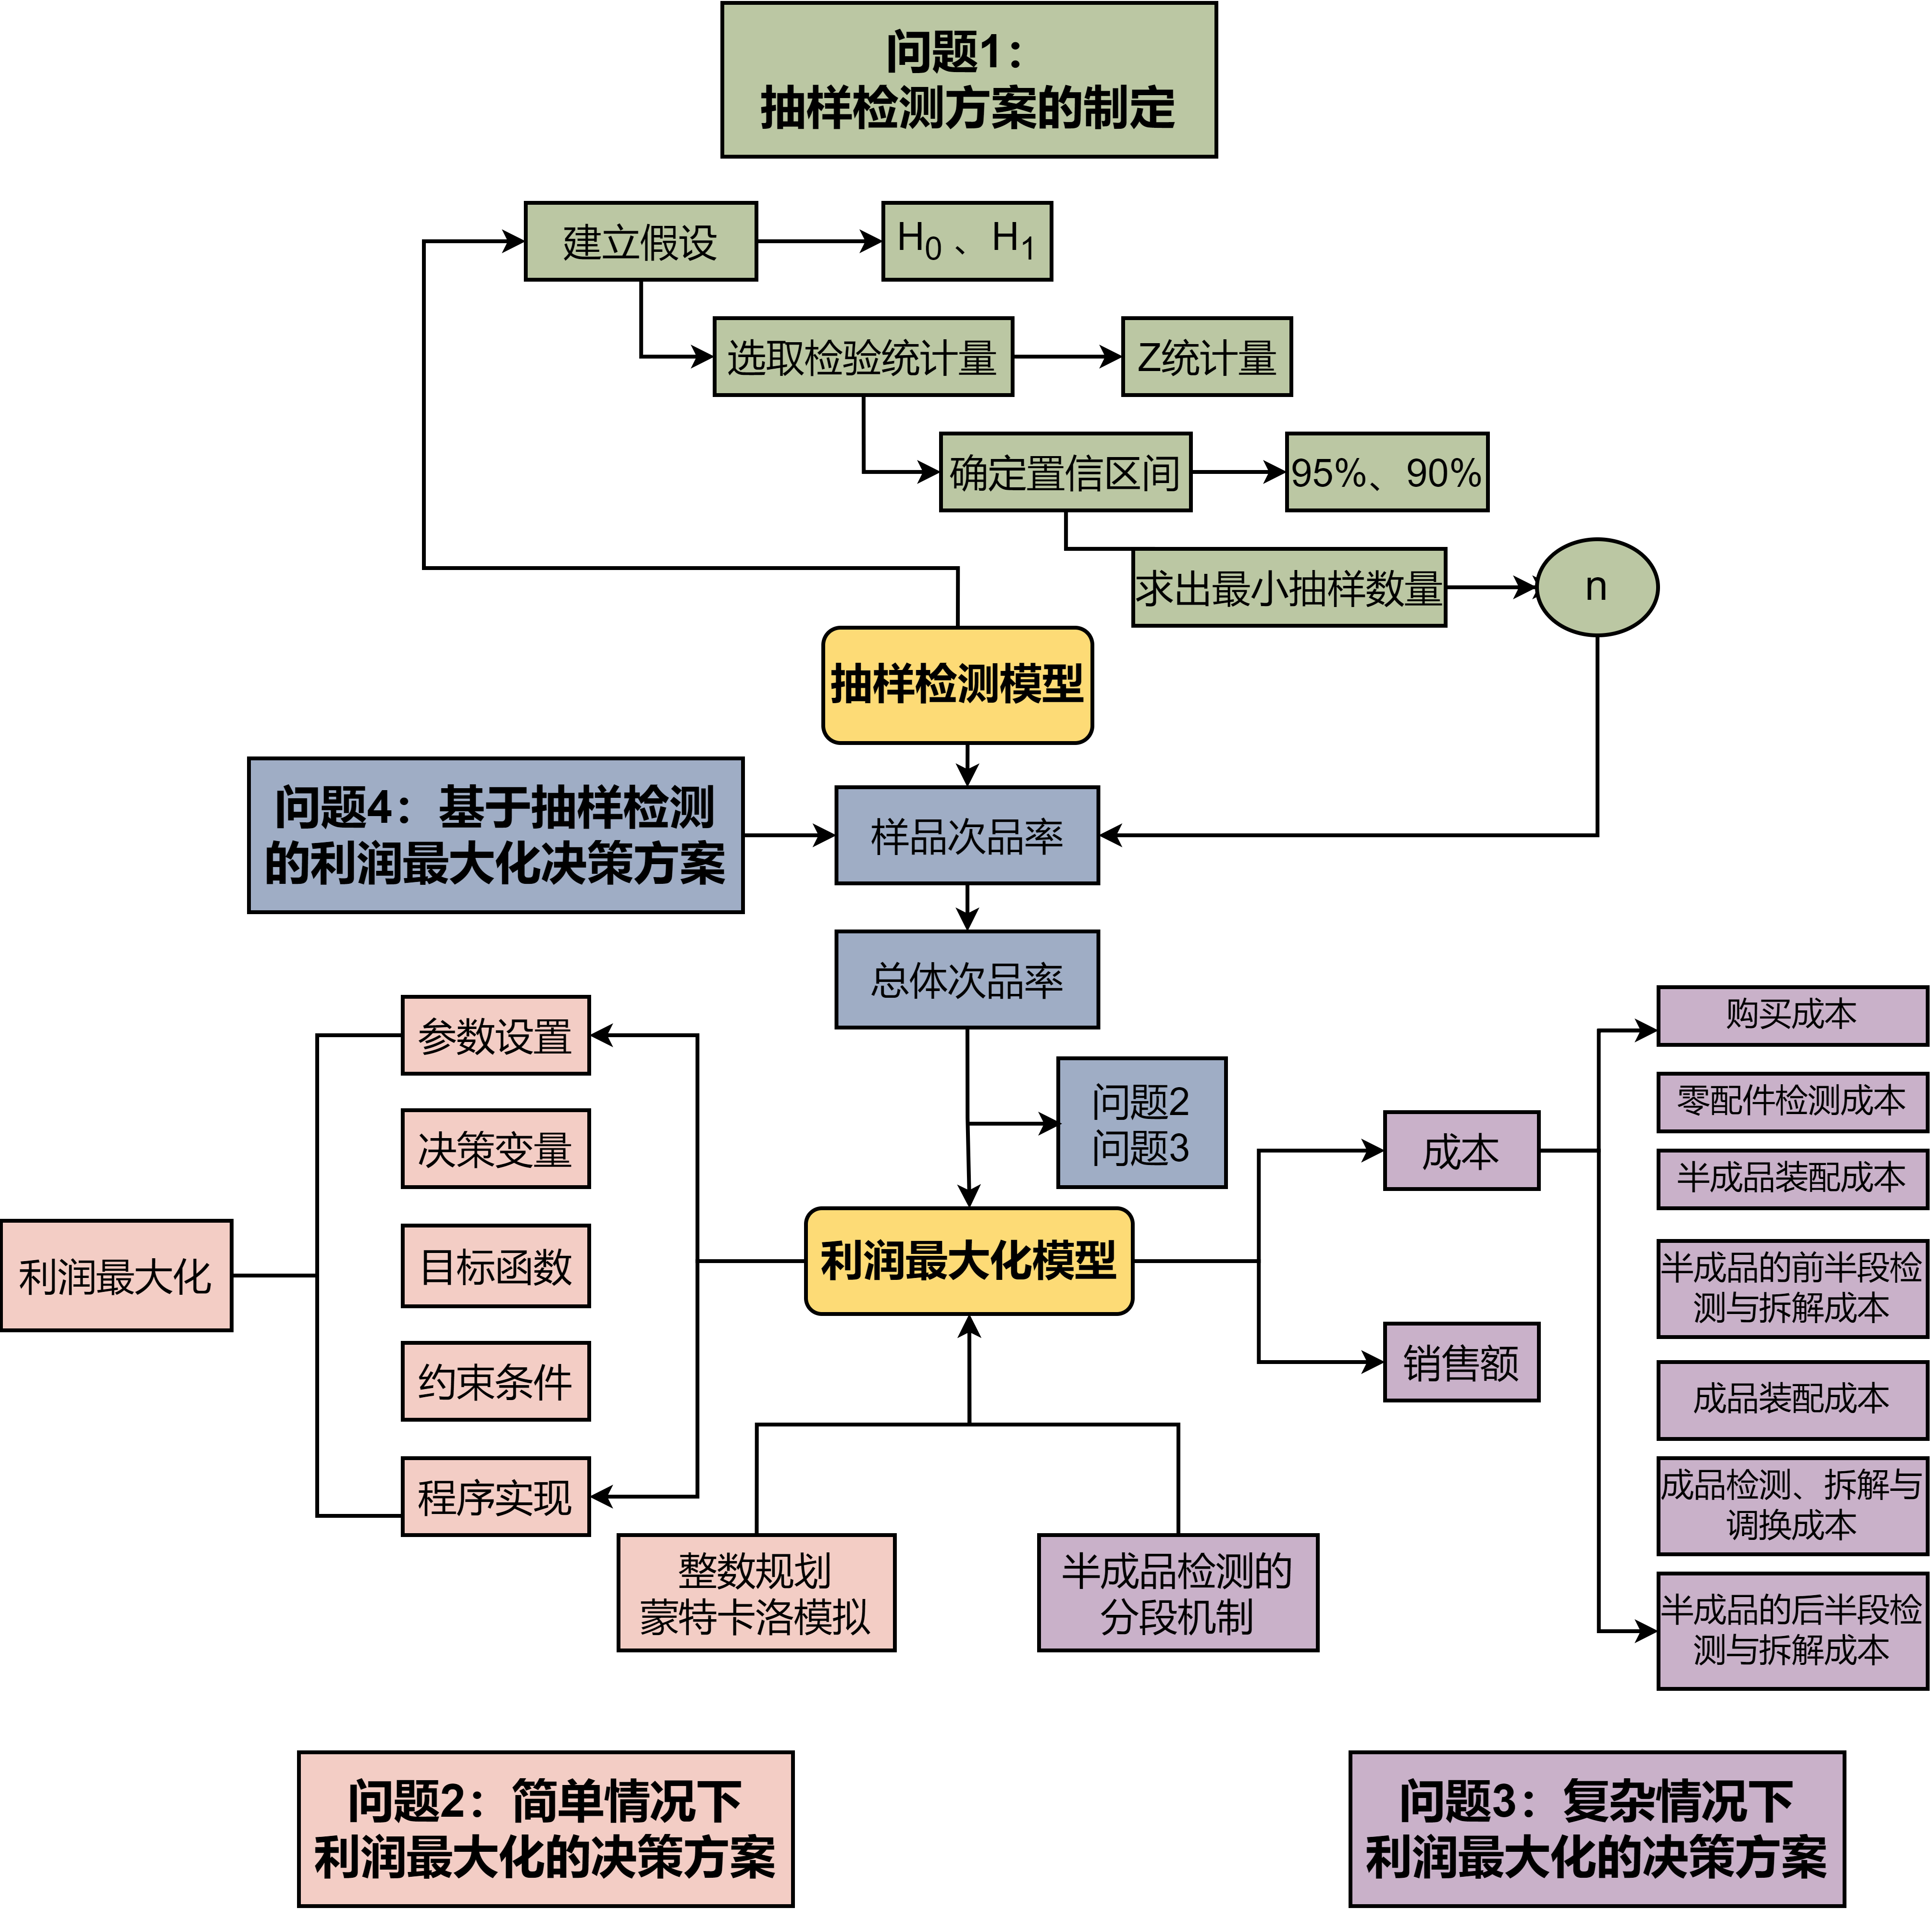
\includegraphics[width=.8\textwidth]{全篇流程图} %图片的名称或者路径之中有空格会出问题  %.8用来调整图片大小
	\caption{本文的研究过程}  
\end{figure}



\section{模型的假设}

本文提出以下合理假设:

\begin{enumerate}[label=\bfseries \arabic*., 
	itemsep=0.5pt, % 条目间距
	topsep=0.5pt, % 列表到上下文的垂直距离
	parsep=0ex]  % 段落间距
	\item 假设每次生产前采购的各种零配件的数量均相等且足够多。
	\item 假设预期次品率通过了假设检验,则使用预期次品率代替零配件总体的实际次品率。
	\item 假设问题1中$\hat{p}$的选取以及问题4中$n$的选取均是合理的。
	\item 假设当在相同情形下,将同种抽样检测方法同时应用到对零配件、半成品和成品的检测上,三种检测的预期和结果是一致的,即零配件次品率=半成品次品率=成品次品率。
\end{enumerate}

\section{符号说明}
\begin{center}
\begin{tabular}{cc}
 \toprule[1.5pt]
 \makebox[0.3\textwidth][c]{符号}	&  \makebox[0.4\textwidth][c]{意义} \\
 \midrule[1pt]
 $ \hat{p} $	    	&  样本次品率\\ 
 $  p$	    	& 真实次品率 \\  
 $ p_0 $	    & 标称值 \\ 
 $ \pi $	    	&  利润  \\ 
 $ W $	    & 销售额  \\ 
 $ c $	    	& 成本 \\ 
 $ c_5 $	    	& 调换成本 \\  
 $ c_{22_1} $	    & 半成品前半段拆解成本 \\ 
 $ c_{22_2} $	    &  半成品后半段拆解成本\\ 
  $ c_{41_1} $	    	& 半成品前半段检测成本 \\  
 $ c_{41_2} $	    & 半成品后半段检测成本 \\ 
 $ N $	    &  产品拆解重组更新后的零配件数量\\ 
\bottomrule[1.5pt]
\end{tabular}
\end{center}

\section{问题1模型的建立和求解}

问题1要求为企业设计一个合理的抽样检测方案,以基于少量样本推断整批零配件的次品率,从而决定接收与否。在情形(1)、(2)中,企业需要分别依据95\%和90\%的置信度,通过抽取样本来判断总体的次品率是否超过供应商提供的标称值10\%。对此,使用统计学中的假设检验方法,建立抽样检测模型,以得到拒收和接收条件,从而制定抽样检测方案。具体步骤如下图所示:

\begin{figure}[htbp]  %h此处,t页顶,b页底,p独立一页,浮动体出现的位置
	\centering  %图表居中
	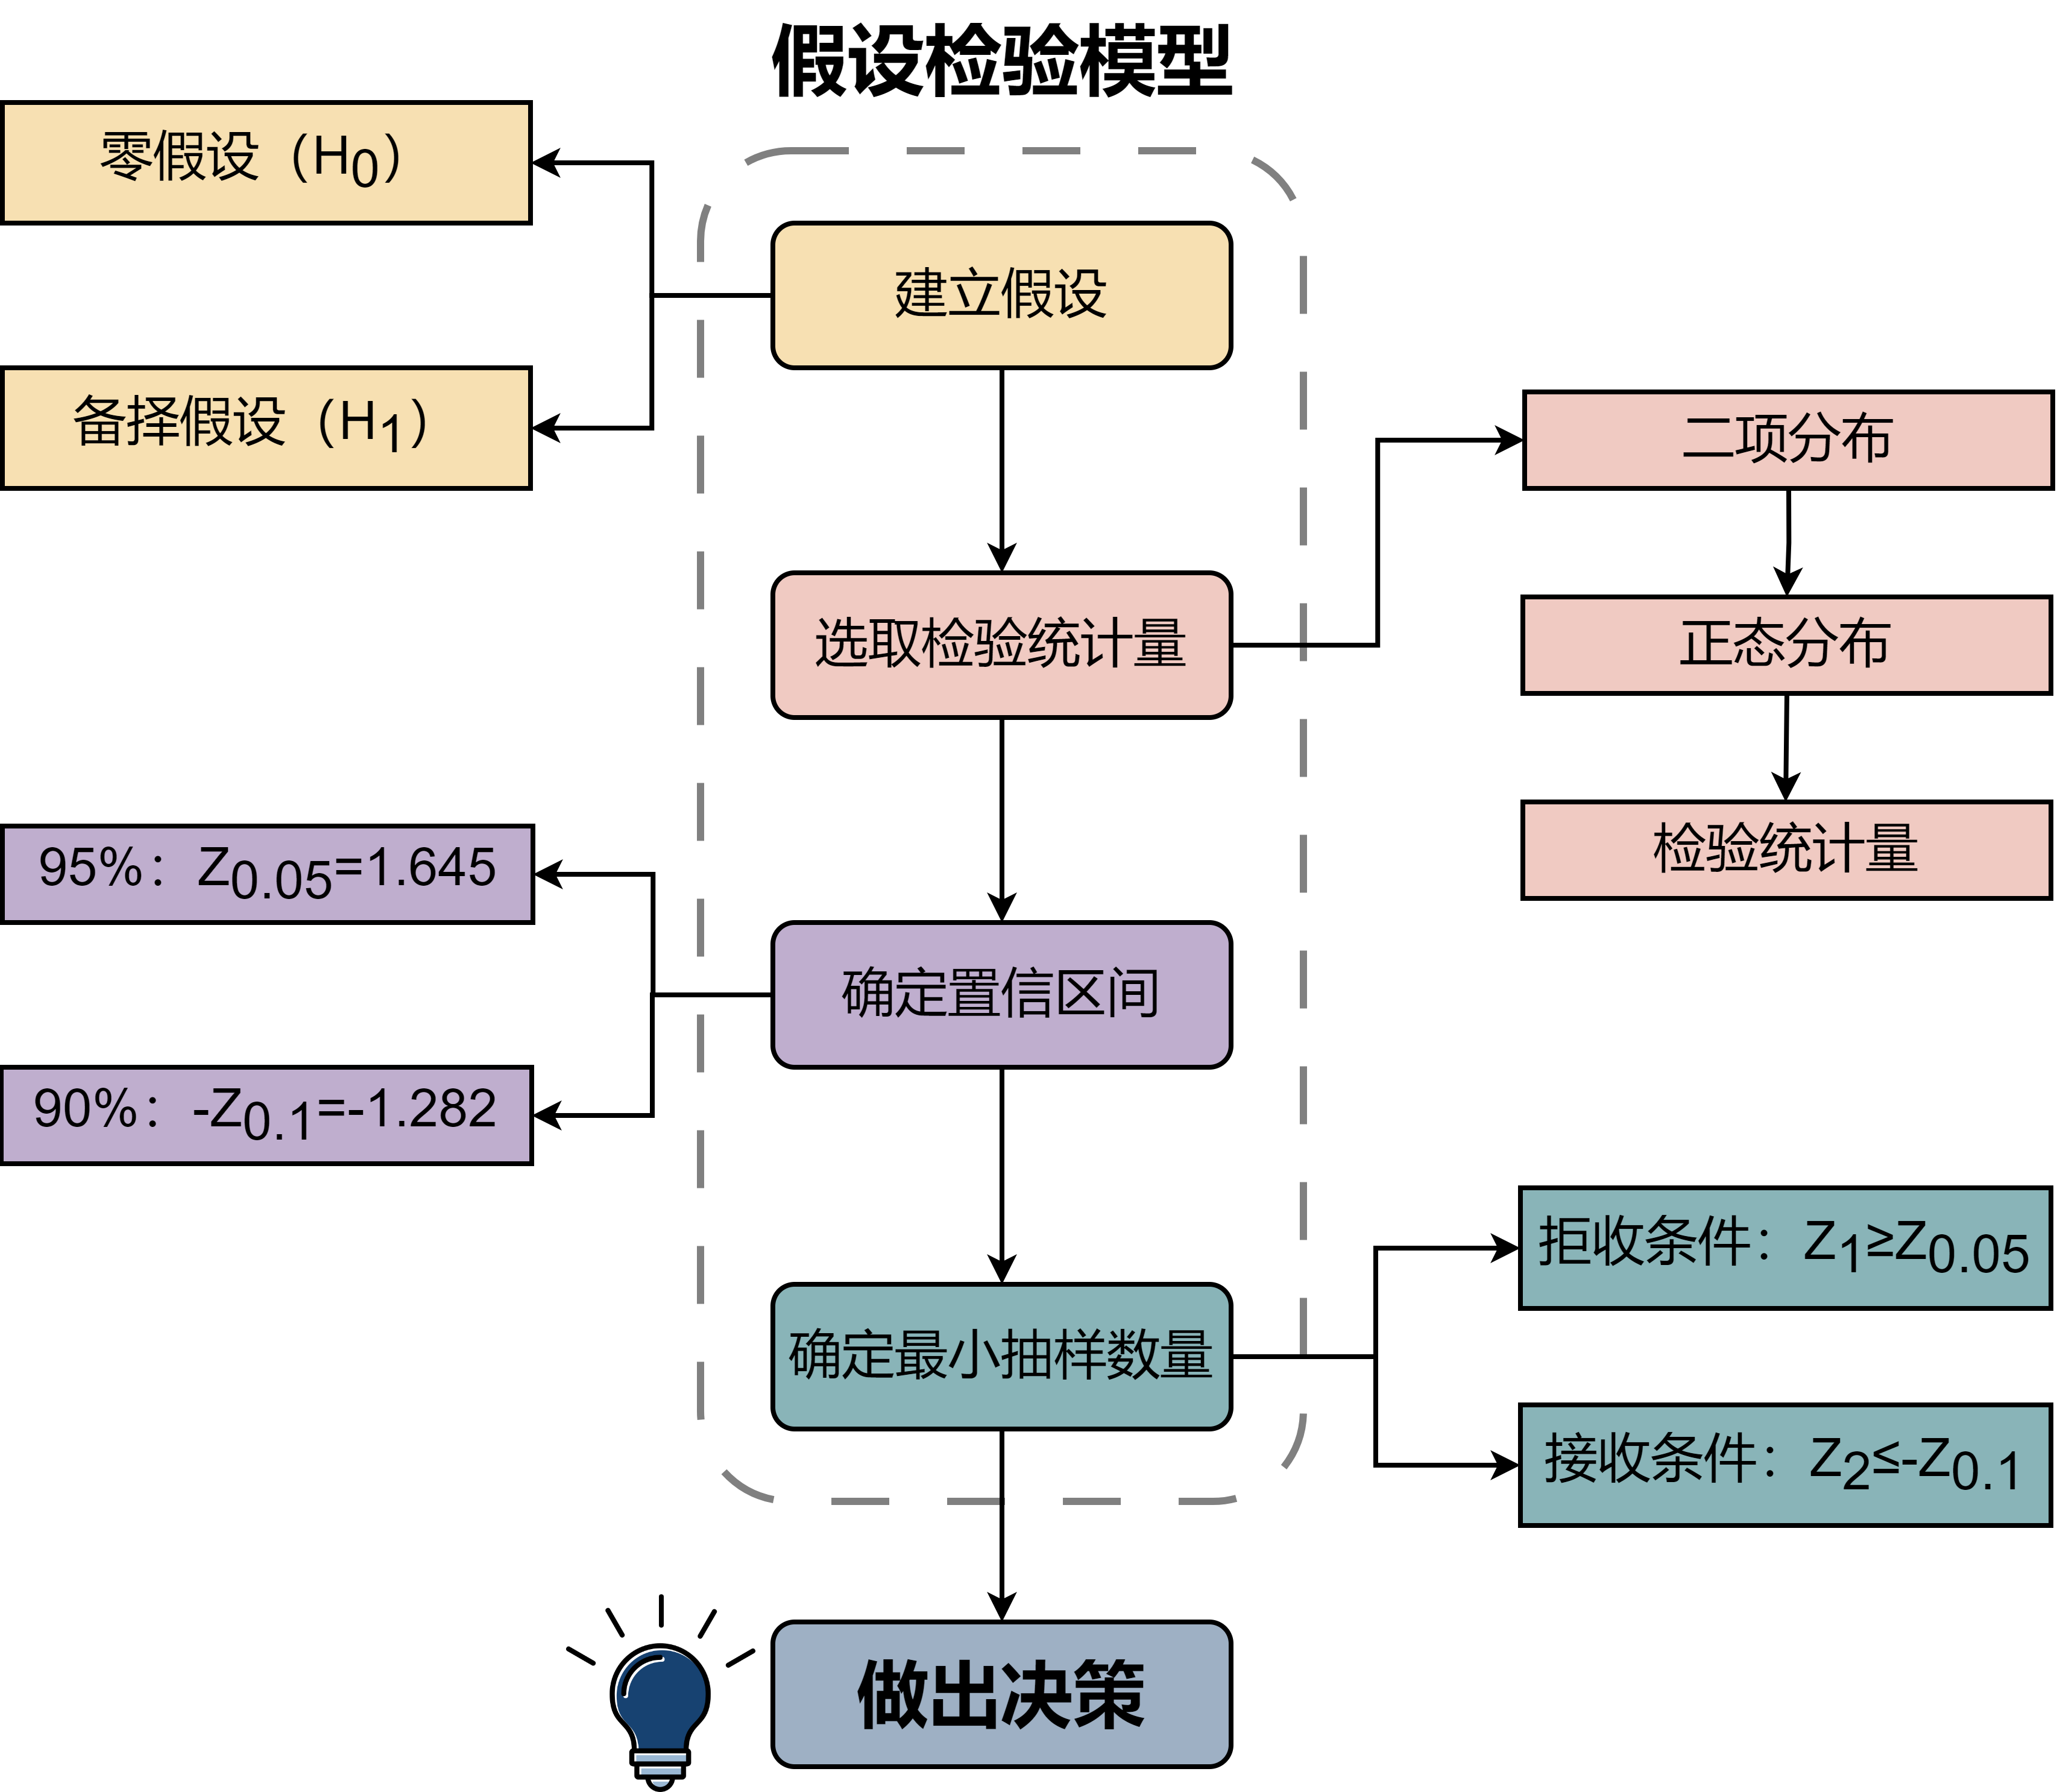
\includegraphics[width=.8\textwidth]{问题一流程} %图片的名称或者路径之中有空格会出问题  %.8用来调整图片大小
	\caption{问题1流程图}  
	\label{pic}
\end{figure}

\subsection{假设检验模型}

根据统计学知识,建立假设检验模型。假设检验运用了反证法和小概率事件原理的思想\cite{SHHT202404019},首先提出零假设$H_0$和备择假设$H_1$,设定显著性水平;再根据数据类型选择合适的检验统计方法,并计算出检验统计量;然后将该值和拒绝域的临界值比较,以判断样本数据与原假设的差异是否显著;最后根据比较结果做出接受或拒绝$H_0$的统计推断。

\subsubsection{建立假设}
原假设和备择假设的建立是假设检验模型的基础。原假设是默认假设,通常表示现状,直到它被证明是错的;备择(研究)假设则是与原假设相矛盾的一个理论\cite{拉森r2004基础统计学},希望通过数据来支持这个假设。根据备择假设方向的不同,假设检验可分为右侧检验、左侧检验、双侧检验三种类型,对应的原假设和备择假设的方向也各不相同。

由题意可知,情形(1)和情形(2)中希望验证的结论方向是相反的,因此需要建立两套方向相反的假设。



\subsubsection{选取检验统计量}

总体次品率可以基于样本次品率来推断。假设抽取的样本量为$n$,其中的次品数为$X$,则样本次品率$\hat{p}$可表示为:

\begin{equation}
	\hat{p}=\frac{X}{n}
\end{equation}

假设样本中零配件的真实次品率为$p$,则合格率为$1-p$。从一批零配件中抽取$n$个样本,则其中次品的数量服从二项分布:

\begin{equation}
	X \sim Binomial(n, p)
\end{equation}

当$n$较大时,根据中心极限定理,该二项分布可近似为正态分布:

\begin{equation}
	X \approx N(n p, n p(1-p))
\end{equation}

将该正态分布标准化,可以得到检验统计量$Z$:

\begin{equation}
	Z=\frac{X-n p_0}{\sqrt{n p_0\left(1-p_0\right)}}
\end{equation}
其中,$p_0$表示供应商提供的标称值(10\%)。

再将该表达式上下同时除以$n$,处理后的$Z$可表示为:

\begin{equation}
	Z=\frac{\hat{p}-p_0}{\sqrt{\frac{p_0\left(1-p_0\right)}{n}}}
\end{equation}

\subsubsection{确定置信区间}

根据问题中95\%和90\%的信度要求,对总体进行单侧假设检验。

在情形(1)中,对于95\%的置信水平,使用标准正态分布的临界值$Z_{0.05}=1.645$。

在情形(2)中,对于90\%的置信水平,使用标准正态分布的临界值$-Z_{0.1}=-1.282$。

\subsection{最少抽样数量的确定}

\subsubsection{情形(1)的最小抽样数量$n_1$}

由题意,构建以下假设:
\begin{align*}
			\text{零假设}H_0:p\leqslant p_0\text{,即零配件次品率不超过标称值,接受零配件 }\\
			\text{备择假设}H_1:p> p_0\text{,即零配件次品率超过标称值,拒绝零配件}
\end{align*}



在95\%的置信度下,若次品率超过10\%,则拒收零配件。拒收条件为$Z_1\geqslant 1.645$,即:

\begin{equation}
	Z_1 = \frac{\hat{p}_1-p_0}{\sqrt{\frac{p_0\left(1-p_0\right)}{n_1}}} \geqslant 1.645
\end{equation}

将$p_0=0.1$代入,得到拒收条件为:

%\begin{equation}
%	\begin{aligned}
%		\hat{p_1} &\geqslant p_0 + 1.645 \times \sqrt{\frac{p_0 (1-p_0)}{n_1}} \\
%		\Rightarrow \hat{p_1} &\geqslant 0.1 + \frac{0.4935}{\sqrt{n_1}}
%	\end{aligned}
%\end{equation}
%
%上式变形可得:
\begin{equation}
	\begin{aligned}
		& n_1 \geqslant\left(\frac{0.4935}{\hat{p_1}-0.1}\right)^2 \\
		\Rightarrow & n_1=\left\lceil\left(\frac{0.4935}{\hat{p_1}-0.1}\right)^2\right\rceil
	\end{aligned}
		\label{拒收}
\end{equation}
其中,$\left\lceil x \right\rceil$表示$x$取不超过$x$的最大整数,下同理。

根据公式\ref{拒收},对于每一个预期的次品率$\hat{p_1}$,可以计算出需要抽取的最小样本量$n_1$,表示若预期次品率超过标称值$(10\%)$,当抽取的样本量为$n_1$时,样本中的次品率已经达到了预期次品率$\hat{p_1}$,则可以在95\%的信度下认定零配件次品率超过标称值,从而拒收这批零配件。

在95\%的信度下,最小抽样数量$n_1$和预期次品率$\hat{p_1}$的函数关系如图\ref{pic.1}所示:

\begin{figure}[htbp]  %h此处,t页顶,b页底,p独立一页,浮动体出现的位置
	\centering  %图表居中
	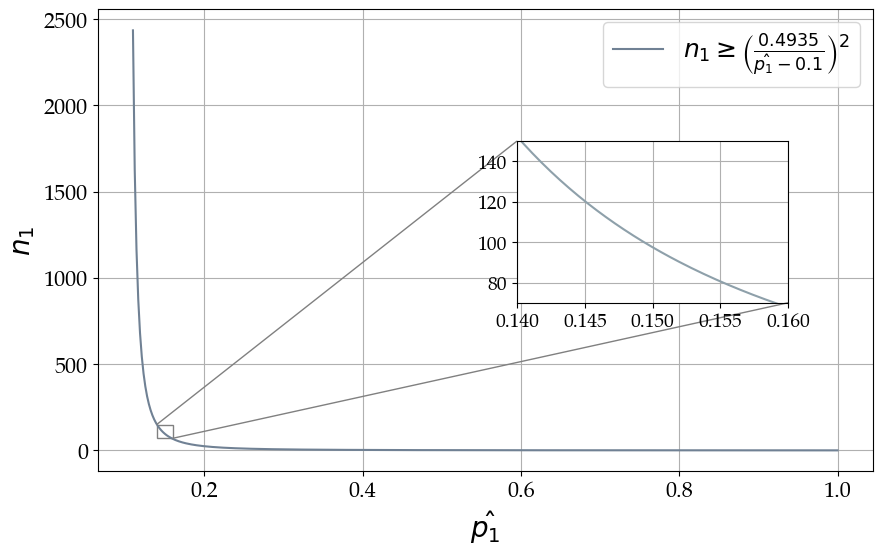
\includegraphics[width=.8\textwidth]{95} %图片的名称或者路径之中有空格会出问题  %.8用来调整图片大小
	\caption{$n_1$和$\hat{p_1}$的函数关系}  
	\label{pic.1}
\end{figure}

上述关系的具体含义是,针对企业对次品率的每一种预期,都可以根据上述表达式求得,为达到一定置信水平所必须进行的最小抽样数量。以点$(\hat{p_1},n_1)$=$(0.15,98)$为例,该点坐标表示,针对企业对于该批零配件高达15\%的预期次品率,此时的抽样检测方案应为抽取并检测98个样本,若发现样本的次品率达到15\%,则可以有95\%的把握认为零配件次品率超过标称值,并予以拒收。


\subsubsection{情形(2)的最小抽样数量$n_2$}

由题意,构建以下假设:
\begin{align*}
	&\text{零假设 }H_0: p \geq p_0\text{,即零配件次品率超过标称值,拒绝零配件} \\
	&\text{备择假设 }H_1: p < p_0\text{,即零配件次品率不超过标称值,接收零配件}
\end{align*}

在90\%的置信度下,若次品率不超过10\%,则接收零配件。接收条件为$Z_2\leqslant -1.282$,即:

\begin{equation}
	Z_2 = \frac{\hat{p_2}-p_0}{\sqrt{\frac{p_0\left(1-p_0\right)}{n_2}}} \leqslant -1.282
\end{equation}

将$p_0=0.1$代入,得到接收条件为:

%\begin{equation}
%	\begin{aligned}
%		\hat{p_2} &\leqslant p_0 - 1.282 \times \sqrt{\frac{p_0 (1-p_0)}{n_2}} \\
%		\Rightarrow \hat{p_2} &\leqslant 0.1 - \frac{0.3846}{\sqrt{n_2}}
%	\end{aligned}
%\end{equation}
%
%上式变形可得:
\begin{equation}
	\begin{aligned}
		& n_2 \geqslant\left(\frac{0.3846}{0.1-\hat{p_2}}\right)^2 \\
		\Rightarrow & n_2=\left\lceil\left(\frac{0.3846}{0.1-\hat{p_2}}\right)^2\right\rceil
	\end{aligned}
		\label{接收}
\end{equation}

根据公式\ref{接收},对于每一个预期的次品率$\hat{p_2}$,可以计算出需要抽取的最小样本量$n_2$,表示若预期次品率不超过标称值(10\%),当抽取的样本量为$n_2$时,样本中的次品率尚未超过预期次品率$\hat{p_2}$,则可以在90\%的信度下认定零配件次品率不超过标称值,从而接收这批零配件。

在90\%的信度下,最小抽样数量$n_2$和预期次品率$\hat{p_2}$的函数关系如图\ref{pic.2}所示:

\begin{figure}[htbp]  %h此处,t页顶,b页底,p独立一页,浮动体出现的位置
	\centering  %图表居中
	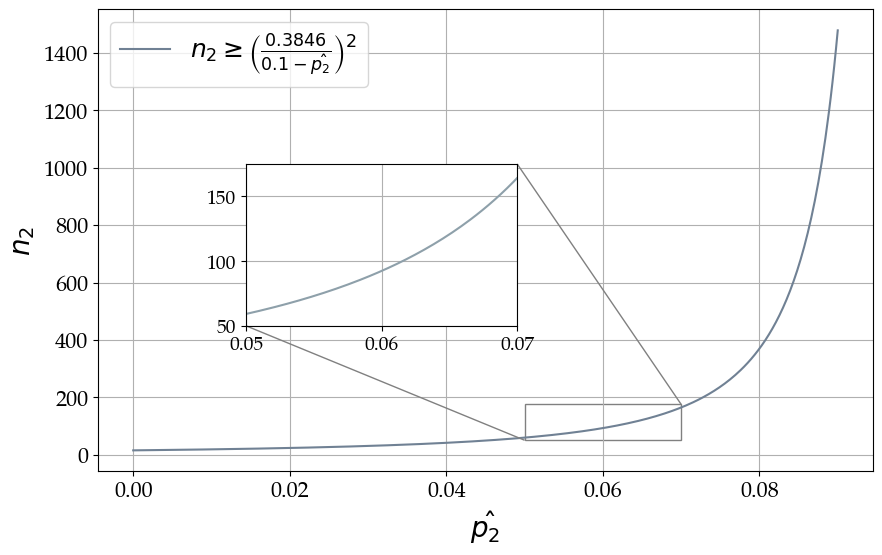
\includegraphics[width=.8\textwidth]{90} %图片的名称或者路径之中有空格会出问题  %.8用来调整图片大小
	\caption{$n_2$和$\hat{p_2}$的函数关系}  
	\label{pic.2}
\end{figure}

同理,上述关系表示,可由企业对次品率的每一种预期,求得在一定置信水平下必须进行的最小抽样数量。以点$(\hat{p_2},n_2)$=$(0.06,93)$为例,该点坐标表示,针对企业对于该批零配件低至6\%的预期次品率,此时的抽样检测方案应为抽取并检测93个样本,若发现样本的次品率只有6\%,则可以有90\%的把握认为零配件次品率不超过标称值,并予以接收。




\section{问题2模型的建立和求解}

问题2要求优化生产过程中考虑零件检测、成品组装、成品检测、拆解以及调换等步骤的决策,旨在最大化利润。对此,综合考虑两种零配件,以及多种可能的成本和收益因素,建立基于整数规划和蒙特卡洛模拟的利润最大化模型,进行决策优化。具体过程如下图所示:

\begin{figure}[htbp]  %h此处,t页顶,b页底,p独立一页,浮动体出现的位置
	\centering  %图表居中
	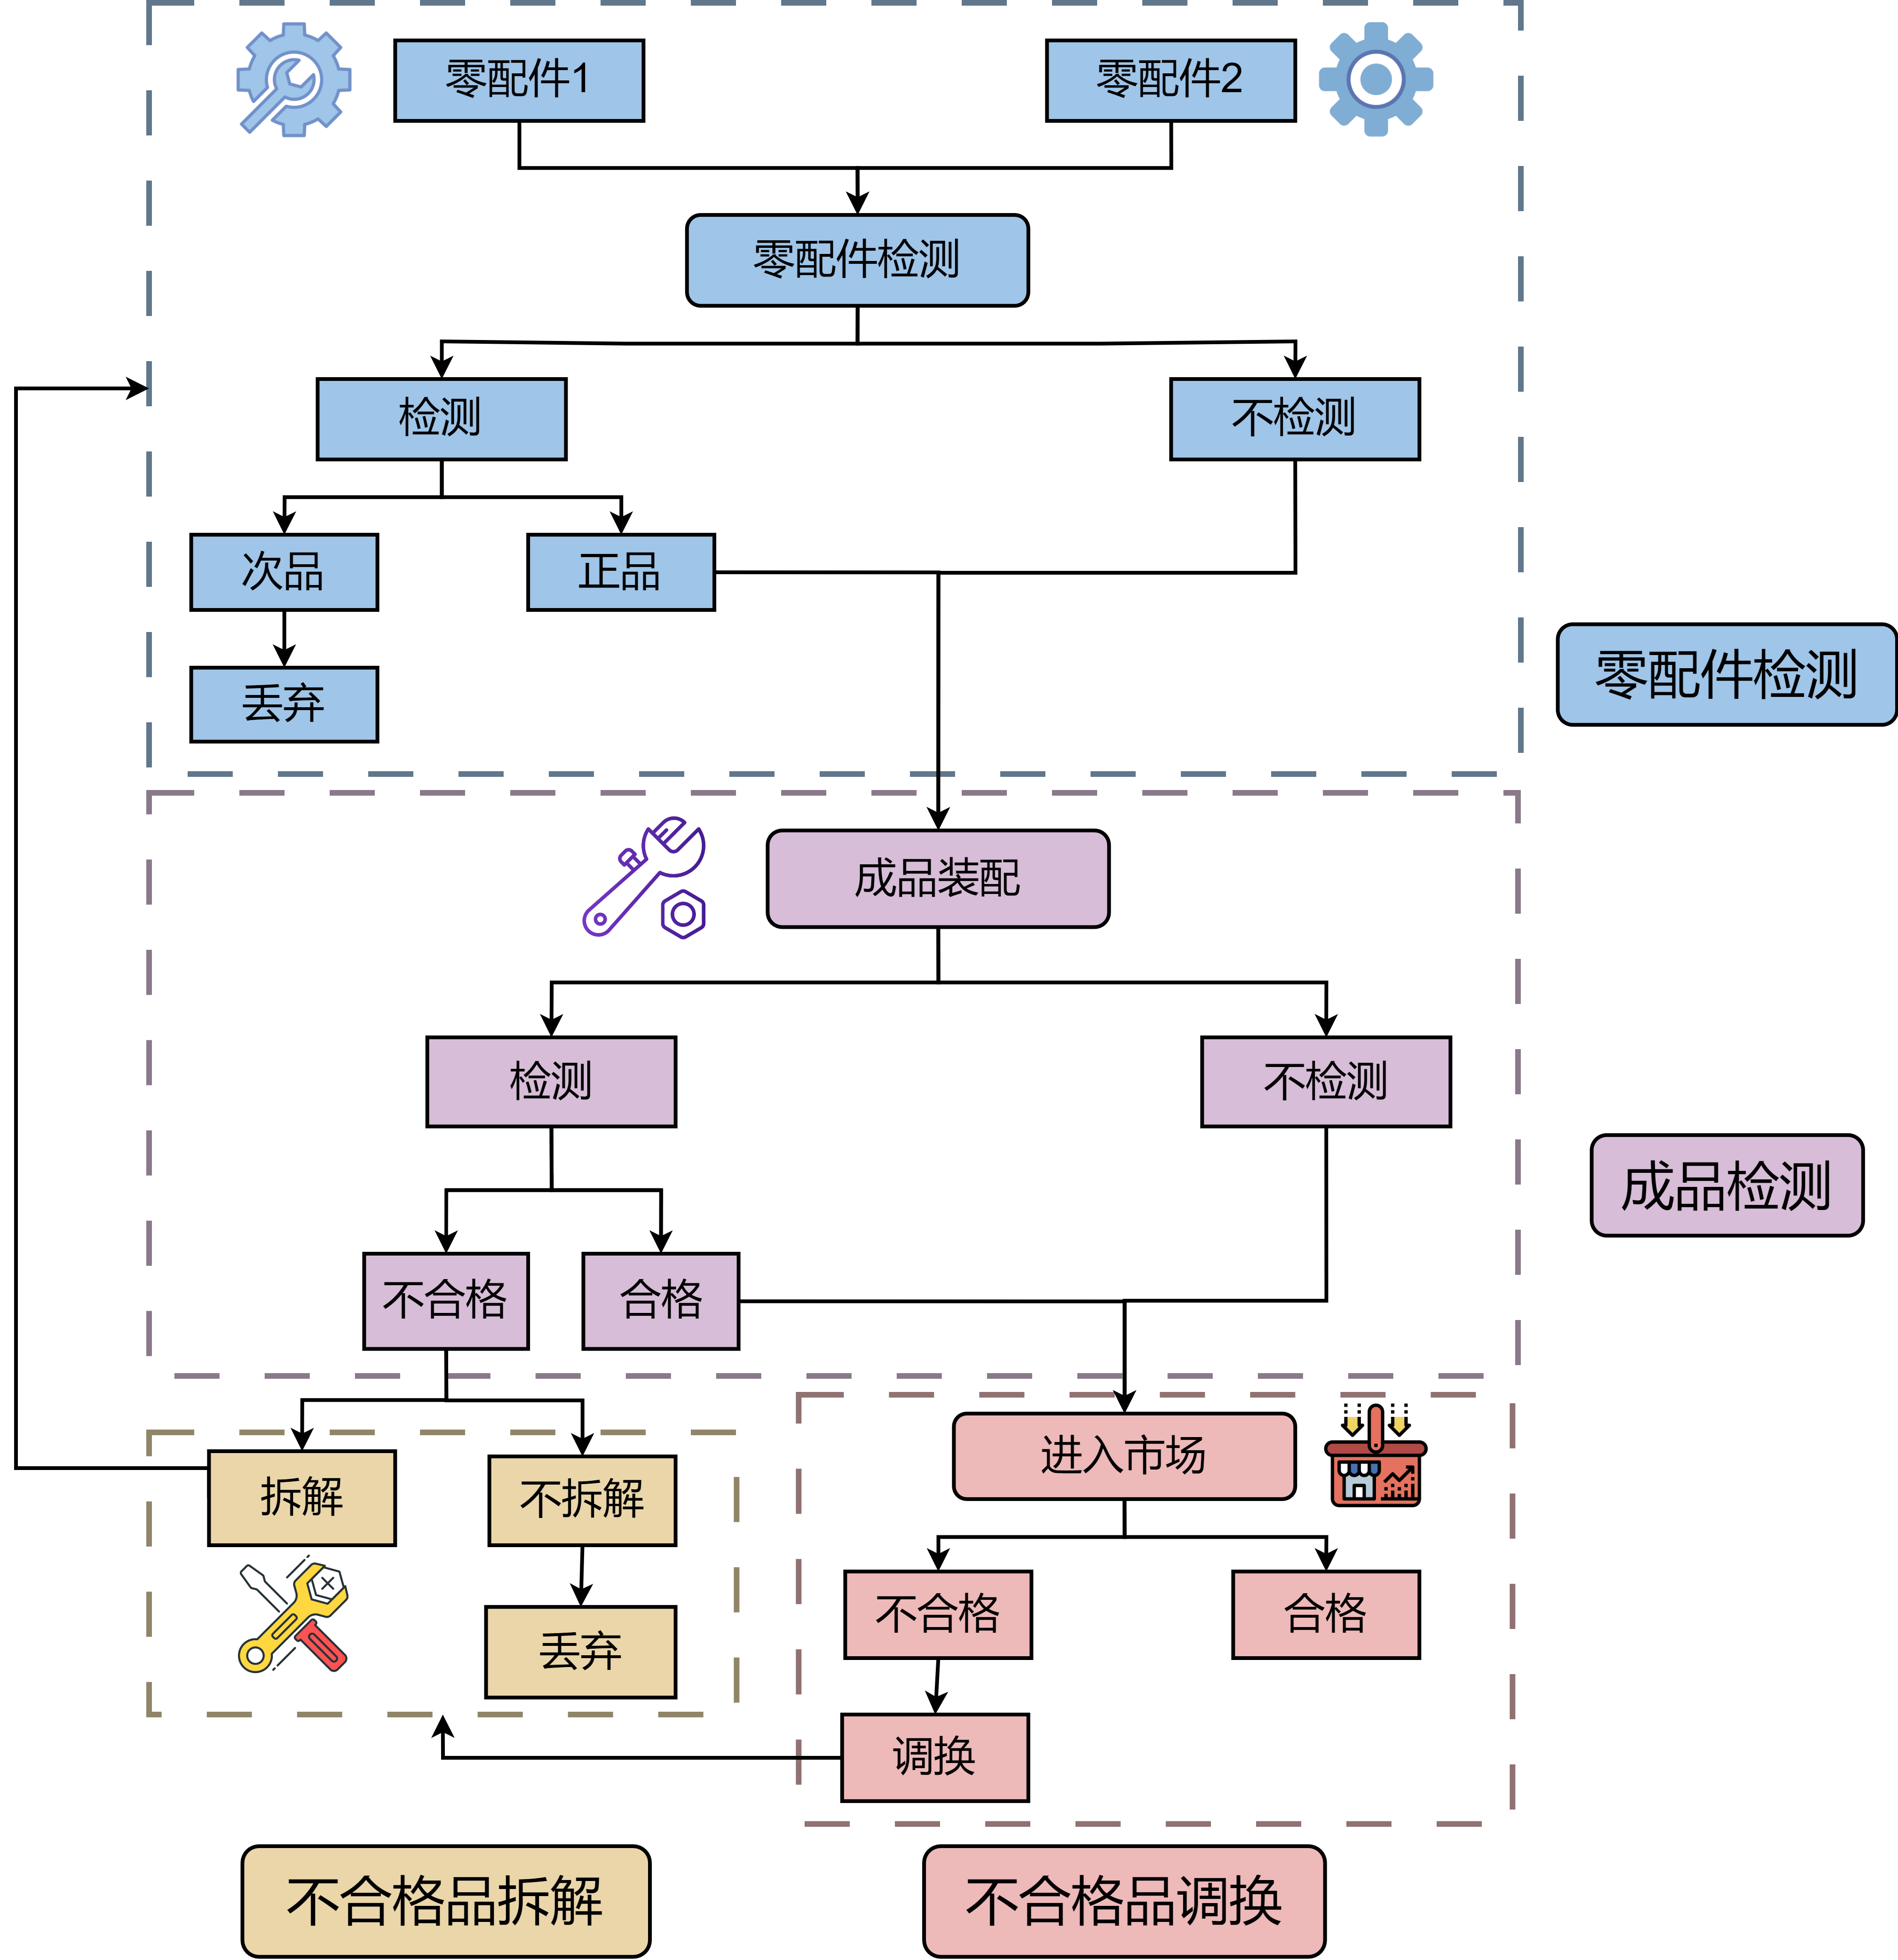
\includegraphics[width=.8\textwidth]{步骤1} %图片的名称或者路径之中有空格会出问题  %.8用来调整图片大小
	\caption{决策过程}  
	\label{pic1}
\end{figure}


\subsection{参数设置}
本模型中涉及的参数如下表所示:

\begin{table}[htbp]
		\centering
	\begin{tabular}{ccc|ccc}
		\toprule[1.5pt]
		类型                   & 符号  & 含义      & 类型                  & 符号 & 含义       \\ \hline
		\multirow{2}{*}{个数}  & $n_1$  & 零配件1个数  & \multirow{9}{*}{单价} & $a_1$ & 零配件1购买单价 \\
		& $n_2$  & 零配件2个数  &                     & $a_2$ & 零配件1单次检测成本 \\ \cline{1-3}
		\multirow{6}{*}{成本}  & $c_1$  & 购买成本    &                     & $a_3$ & 零配件2购买单价 \\
		& $c_{21}$ & 零配件检测成本 &                     & $a_4$ & 零配件2单次检测成本 \\
		& $c_{22}$ & 成品检测成本  &                     & $a_5$ & 单次装配成本     \\
		& $c_3$  & 装配成本    &                     & $a_6$ & 成品单次检测成本   \\
		& $c_4$  & 拆解成本    &                     & $a_7$ & 市场零售价   \\
		& $c_5$  & 调换成本    &                     & $a_8$ & 单次调换成本   \\ \cline{1-3}
		\multirow{3}{*}{次品率} & $q_1$  & 零配件1次品率 &                     & $a_9$ & 单次拆解费用   \\  
		& $q_2$  & 零配件2次品率 &                     &    &          \\
		& $q_3$  & 成本不合格率  &                     &    &          \\ \bottomrule[1.5pt]
	\end{tabular}
\end{table}

根据假设,为简化模型,降低计算复杂程度,令零配件1和零配件2的个数相等,即$n_1=n_2=n$。

\subsection{决策变量}
在产品的装配与生产过程中,企业需要对是否检测零配件,是否检测成品,是否拆解不合格成品等环节作出合理决策。分别设定整数规划的决策变量如下:

\begin{equation}
	\begin{aligned}
		D_1 & =\left\{\begin{array}{l}
			1 , \text{零配件1进行检测}\\
			0 , \text{零配件1不进行检测}
		\end{array}\right. \\
		D_2 & =\left\{\begin{array}{l}
			1 , \text{零配件2进行检测}\\
			0 , \text{零配件2不进行检测}
		\end{array}\right. \\
		E & =\left\{\begin{array}{l}
			1 , \text{成品进行检测} \\
			0 , \text{成品不进行检测}
		\end{array}\right. \\
		F & =\left\{\begin{array}{l}
			1 , \text{成品进行拆解} \\
			0 , \text{成品不进行拆解}
		\end{array}\right.
	\end{aligned}
\end{equation}

\subsection{目标函数与约束条件}

本模型的目标是实现利润最大化。利润$\pi$可表示为:

\begin{equation}
	\pi=W-C
	\label{pai}
\end{equation}
其中,$W$表示销售额,并已经考虑了次品可能流入市场后对消费者进行的补偿;$C$表示总成本。

\subsubsection{成本计算}
在本问题中,产品的组装和生产过程共包含五步决策,分别为:零配件检测、成品装配、成品检测、不合格品拆解与不合格品调换。每个步骤都会产生相应的成本,包括购买成本、零部件和产品的检测成本、装配成本、拆解成本和调换成本。

具体的决策步骤如下所示:

\subsubsection*{步骤一:零配件检测}

对零件进行检测后,只有检测合格的零配件才能进入成品装配环节,检测不合格的零配件会被丢弃,造成该种零配件个数减少。

经过零配件检测后的零配件数量可由以下公式求得:

\begin{equation}
	\left\{\begin{array}{l}
		n _1^*=(1-D _1 \cdot q_1 ) \cdot n _1 \\
		n _2^*=(1-D_ 2 \cdot q_2) \cdot n_ 2
	\end{array}\right.
\end{equation}
其中,$n_1^*$、$n_2^*$分别表示零配件检测后零配件1、2的个数。

将正品和次品零配件分开统计,得到如下公式:

\begin{equation}
	\left\{\begin{array}{l}
		n _1^*=(1-q _1) \cdot n _1+(1-D _1) \cdot q _1 \cdot n _1 \\
		n _2^*=(1-q _2) \cdot n_ 2+(1-D_ 2) \cdot q _2 \cdot n_ 2
	\end{array}\right.
\end{equation}
其中,$(1-q _1) \cdot n _1$是正品零配件1个数,$(1-D _1) \cdot q _1 \cdot n _1$是次品零配件1个数;$(1-q _2) \cdot n_ 2$是正品零配件2个数,$(1-D_ 2) \cdot q _2 \cdot n_ 2$是次品零配件2个数。

由上述分析可知,零配件检测的总成本$C_{21}$可表示为:

\begin{equation}
	C_{21}=n_1\cdot D_1\cdot
	a_2+n_2 \cdot D_2 \cdot a_4 
	\label{C}
\end{equation}

\subsubsection*{步骤二:成品装配}

由于假定企业购进的零配件1和零配件2总数相同,而两种零配件在步骤一中被测定为次品并丢弃的数量可能不同,故在成品装配的过程中,其中一种零配件可能冗余。因此,规定成品装配过程按以下原则进行:

(1)尽可能装配更多的成品,直到其中一种零配件耗尽为止。

(2)由于根据假设,购进的零配件数量足够多,按照“以频率估计概率”原则确定装配成成品的零配件质量。

按照上述原则装配成品,并不妨令$n_1^* \geqslant n_2^*$($n_1^* < n_2^*$时同理),此时可装配成品共$n_2^*$个,每个成品的零配件构成如下:

\begin{table}[htbp]
			\centering
				\caption{成品装配后的零配件构成}
	\begin{tabular}{cccc}
		\toprule[1.5pt]
		\multirow{2}{*}{成品}   & \multicolumn{2}{c}{构成} & \multirow{2}{*}{数量} \\ \cline{2-3}
		& 零配件1       & 零配件2      &                     \\ \hline
		合格品                   & 正品         & 正品        & $(1-q _2) \cdot n _2 \cdot \frac{1-q _1}{1-D_ 1 \cdot q _1}$                   \\ \hline
		\multirow{3}{*}{不合格品} & 次品         & 正品        & $(1-q _2) \cdot n _2 \cdot \frac{(1-D _1) \cdot q _1}{1-D _1 \cdot q _1}$                   \\
		& 正品         & 次品        & $(1-D _2) \cdot q _2 \cdot n _2 \cdot \frac{1-q _1}{1-D_ 1 \cdot q _1}$                   \\
		& 次品         & 次品        & $(1-D_ 2) \cdot q_ 2 \cdot n _2 \cdot \frac{(1-D_ 1) \cdot q_ 1}{1-D_ 1 \cdot q _1}$                   \\ \bottomrule[1.5pt]
	\end{tabular}
\end{table}

由上述分析可知,成品装配成本$C_3$可表示为:

\begin{equation}
	C_3=n_2^*\cdot a_5 
\end{equation}

\subsubsection*{步骤三:成品检测}

成品检测的总成本$C_{22}$可表示为:

\begin{equation}
	C_{22} = n_2^* \cdot E \cdot a_6
\end{equation}

经过成品检测后的产品构成为:

\begin{table}[htbp]
				\centering
								\caption{成品检测后的产品构成}
	\begin{tabular}{cccc}		
		\toprule[1.5pt]
		\multirow{2}{*}{成品}   & \multicolumn{2}{c}{构成} & \multirow{2}{*}{数量} \\ \cline{2-3}
		& 零配件1       & 零配件2      &                     \\ \hline
		合格品                   & 正品         & 正品        & $(1-q_ 3) \cdot(1-q _2) \cdot n _2 \cdot \frac{1-q _1}{1-D _1 \cdot q _1}$                   \\\hline
		\multirow{4}{*}{不合格品} & 正品         & 正品        & $q _3 \cdot(1-q _2) \cdot n_ 2 \cdot \frac{1-q_ 1}{1-D_ 1 \cdot q _1}$                   \\
		& 次品         & 正品        & $(1-q_ 2) \cdot n _2 \cdot \frac{(1-D _1) \cdot q _1}{1-D_ 1 \cdot q_ 1}$                  \\
		& 正品         & 次品        & $(1-D_ 2) \cdot q _2 \cdot n _2 \cdot \frac{1-q _1}{1-D _1 \cdot q _1}$                   \\
		& 次品         & 次品        & $(1-D_ 2) \cdot q _2 \cdot n _2 \cdot \frac{(1-D _1) \cdot q_ 1}{1-D _1 \cdot q_ 1}$                   \\ \bottomrule[1.5pt]
	\end{tabular}
\end{table}

\subsubsection*{步骤四:不合格品拆解}

由题意可知,被拆解的不合格成品的可能来源有两个,一是经成品检测发现的不合格品,二是未经成品检测被投入市场后被买家退回的不合格品,故拆解与否与成品检测与否没有必然联系,而所有不合格品都会参与拆解决策。因此,不合格品的拆解成本$C_4$可表示为:

\begin{equation}
    C_4 = F \cdot [n_2^* - \frac{(1 - q_1)(1 - q_2)(1 - q_3) \cdot n_2}{1 - D_1 \cdot q_1}]\cdot a_9
\end{equation}

\subsubsection*{步骤五:不合格品调换}
由于未经成品检测而流入买家手中的不合格品将被要求调换,从而产生调换成本。调换成本$C_5$可表示为:

\begin{equation}
	C_5 = (1 - E) \cdot [n_2^* - \frac{(1 - q_1)(1 - q_2)(1 - q_3) \cdot n_2}{1 - D_1 \cdot q_1}]\cdot a_8
\end{equation}

综合上述五个步骤的分析,一次完整的决策过程的最终成本$C$可表示为:

\begin{equation}
    C = C_1 + C_{21} + C_{22} + C_3 + C_4 + C_5
\end{equation}

\subsubsection{销售额计算}

考虑买家若收到不合格品将有退换要求,可将经过步骤三:成品检测后的合格品分为两类,分别为:

(1)卖给买家的合格品;

(2)以补偿形式为买家退还不合格品的合格品。

因此,产品的销售额$W$可表示为:

\begin{equation}
	W=(1-q _2) \cdot(1-q _3) \cdot n _2 \cdot \frac{1-q _1}{1-D _1 \cdot q _1} \cdot a _7
	\label{W}
\end{equation}

结合公式\ref{pai}、公式\ref{C}和公式\ref{W},可求得最终利润$\pi$。

\subsubsection{后续决策的数值更新}
第一轮决策结束后,如果进行不合格品拆解,经过拆解的零配件会进入第二轮决策,故第二轮决策中的零配件个数和次品率会发生变化。

其一,更新零配件个数。$n_{21}$、$n_{22}$分别表示经过拆解进入第二轮决策的零配件1和零配件2的个数,可表示为:

\begin{equation}
	n_{21}=n_{22}=N=n_2^*-\frac{\left(1-q_1\right)\left(1-q_2\right)\left(1-q_3\right) \cdot n_2}{1-D_1 \cdot q_1}
\end{equation}

其二,更新次品率。$q_{21}$、$q_{22}$分别表示第二轮决策中零配件1和零配件2的次品率,可表示为:

\begin{equation}
	\begin{aligned}
		& q_{21}=\frac{\frac{\left(1-D_1\right)\left(1-q_2\right) \cdot q_1 \cdot n_2}{1-D_1 q_1}+\frac{\left(1-D_1\right)\left(1-D_2\right) \cdot q_1 \cdot q_2 \cdot n_2}{1-D_1 q_1}}{N} \\
		& q_{22}=\frac{\frac{\left(1-D_2\right)\left(1-q_1\right) \cdot q_2 \cdot n_2}{1-D_1 \cdot q_1}+\frac{\left(1-D_1\right)\left(1-D_2\right) \cdot q_1 \cdot q_2 \cdot n_2}{1-D_1 \cdot q_1}}{N}
	\end{aligned}
\end{equation}


\subsection{程序设计与实现}

利用Python设计程序,进行蒙特卡洛模拟,计算并记录每轮利润,逐步寻找实现利润最大化的最优策略。

由于当循环次数过多时,利润的增长变得非常缓慢,且决策过程更加复杂,因此设置循环阈值$\gamma = 5$。此外,在遍历程序时发现,遍历1000次和10000次时最终利润有较大出入,而遍历10000次和100000次时最终利润相差无几,因此选择对程序遍历10000次,得到最终利润。同时,结合实际情况,在其他条件不变的情况下,企业会尽可能地减少工作量,因此在多种决策方案的利润相近时,选择过程更简单的决策方案。具体代码见附录。

综合以上分析,针对表1企业在生产中遇到的六种情形,给出的决策方案如下表所示:
\begin{table}[htbp]
	\centering
					\caption{问题2的决策方案}
		 \scalebox{0.62}{
	\begin{tabular}{c|c|cccc|cccc|cccc}
		\toprule[1.5pt]
		\multirow{2}{*}{情况} & \multirow{2}{*}{最终利润} & \multicolumn{4}{c|}{第一轮决策}                                                                                                                                                                                  & \multicolumn{4}{c|}{第二轮决策}                                                                                                                                                                                  & \multicolumn{4}{c}{第三轮决策}                                                                                                                                                                                   \\ \cline{3-14} 
		&                       & \begin{tabular}[c]{@{}c@{}}零配件1\\ 检测\end{tabular} & \begin{tabular}[c]{@{}c@{}}零配件2\\ 检测\end{tabular} & \begin{tabular}[c]{@{}c@{}}成品\\ 检测\end{tabular} & \begin{tabular}[c]{@{}c@{}}不合格品\\ 拆解\end{tabular} & \begin{tabular}[c]{@{}c@{}}零配件1\\ 检测\end{tabular} & \begin{tabular}[c]{@{}c@{}}零配件2\\ 检测\end{tabular} & \begin{tabular}[c]{@{}c@{}}成品\\ 检测\end{tabular} & \begin{tabular}[c]{@{}c@{}}不合格品\\ 拆解\end{tabular} & \begin{tabular}[c]{@{}c@{}}零配件1\\ 检测\end{tabular} & \begin{tabular}[c]{@{}c@{}}零配件2\\ 检测\end{tabular} & \begin{tabular}[c]{@{}c@{}}成品\\ 检测\end{tabular} & \begin{tabular}[c]{@{}c@{}}不合格品\\ 拆解\end{tabular} \\ \hline
		1                   & 15.55n                & 否                                                 & 否                                                 & 否                                               & 是                                                 & 是                                                 & 是                                                 & 是                                               & 是                                                 & 否                                                 & 否                                                 & 否                                               & 否                                                 \\
		2                   & 6.31n                 & 是                                                 & 是                                                 & 否                                               & 是                                                 & 否                                                 & 否                                                 & 否                                               & 是                                                 & 否                                                 & 否                                                 & 是                                               & 否                                                 \\
		3                   & 13.70n                & 否                                                 & 否                                                 & 是                                               & 是                                                 & 是                                                 & 是                                                 & 是                                               & 是                                                 & 否                                                 & 否                                                 & 是                                               & 否                                                 \\
		4                   & 9.20n               & 是                                                 & 是                                                 & 是                                               & 是                                                 & 否                                                 & 否                                                 & 是                                               & 是                                                 & 否                                                 & 是                                                 & 是                                               & 否                                                 \\
		5                   & 8.49n                 & 否                                                 & 否                                                 & 是                                               & 是                                                 & 否                                                 & 是                                                 & 是                                               & 是                                                 & 否                                                 & 否                                                 & 是                                               & 否                                                 \\
		6                   & 18.59n                & 否                                                 & 否                                                 & 否                                               & 否                                                 & -                                                 & -                                                 & -                                               & -                                                 & -                                                 & -                                                 & -                                               & -                                                 \\ 	\bottomrule[1.5pt]
	
	\end{tabular}
} \label{biao1}
\end{table}



\section{问题3模型的建立和求解}
问题3是对问题2的扩展,需要考虑的零配件数量增加,检测策略也更加复杂,其目的仍然是通过合理决策,最大化最终成品的利润。对此,利用整数规划来描述不同阶段的检测、装配、拆解与调换的优化过程,并改进问题2中的基于整数规划和蒙特卡洛模拟的最大利润模型,以得到决策方案。

\subsection{模型假设}
由表2可知,8种零配件的次品率相同,且检测成本相差无几。结合对问题2中得到的6种情况下最优决策方案的分析,构成同一种成品的零配件(零配件1和零配件2)是否检测的决策往往是同步的。因此,为了简化决策的复杂程度,假设零配件1、2、3(共同构成半成品1),零配件4、5、6(共同构成半成品2)和零配件7、8(共同构成半成品3)的检测策略保持一致。

同时,在本问题中,仍然假定每种零配件的初始数量相同,令之为单位1,即:
\begin{equation}
	n_1 = n_2 = n_3 = n_4 = n_5 = n_6 = n_7 = n_8 = 1
	\end{equation}
	
\subsection{半成品检测的分段机制}
在本模型中引入半成品检测的分段机制,即按照半成品来源的不同将其分为两个部分,各个部分的检测决策独立确定。

根据生产流程,半成品的来源有二,分别是由零配件装配成的半成品,和由成品拆解成的半成品。因此,将半成品按来源分为两个部分,由此将对半成品的检测分为前后两个阶段,前半段表示对由零配件装配成的半成品进行检测,后半段表示对由成品拆解成的半成品进行检测,有效地在前半段避免了资源浪费问题,简化了生产流程,并在后半段确保了成品的质量。

\subsection{模型建立}
\subsubsection{成本计算}
本模型中的成本包括购买成本、检测成本、装配成本、拆解成本和调换成本等多个方面,再结合半成品检测的分段机制,具体的成本构成如下图所示:

\begin{figure}[htbp]  %h此处,t页顶,b页底,p独立一页,浮动体出现的位置
	\centering  %图表居中
	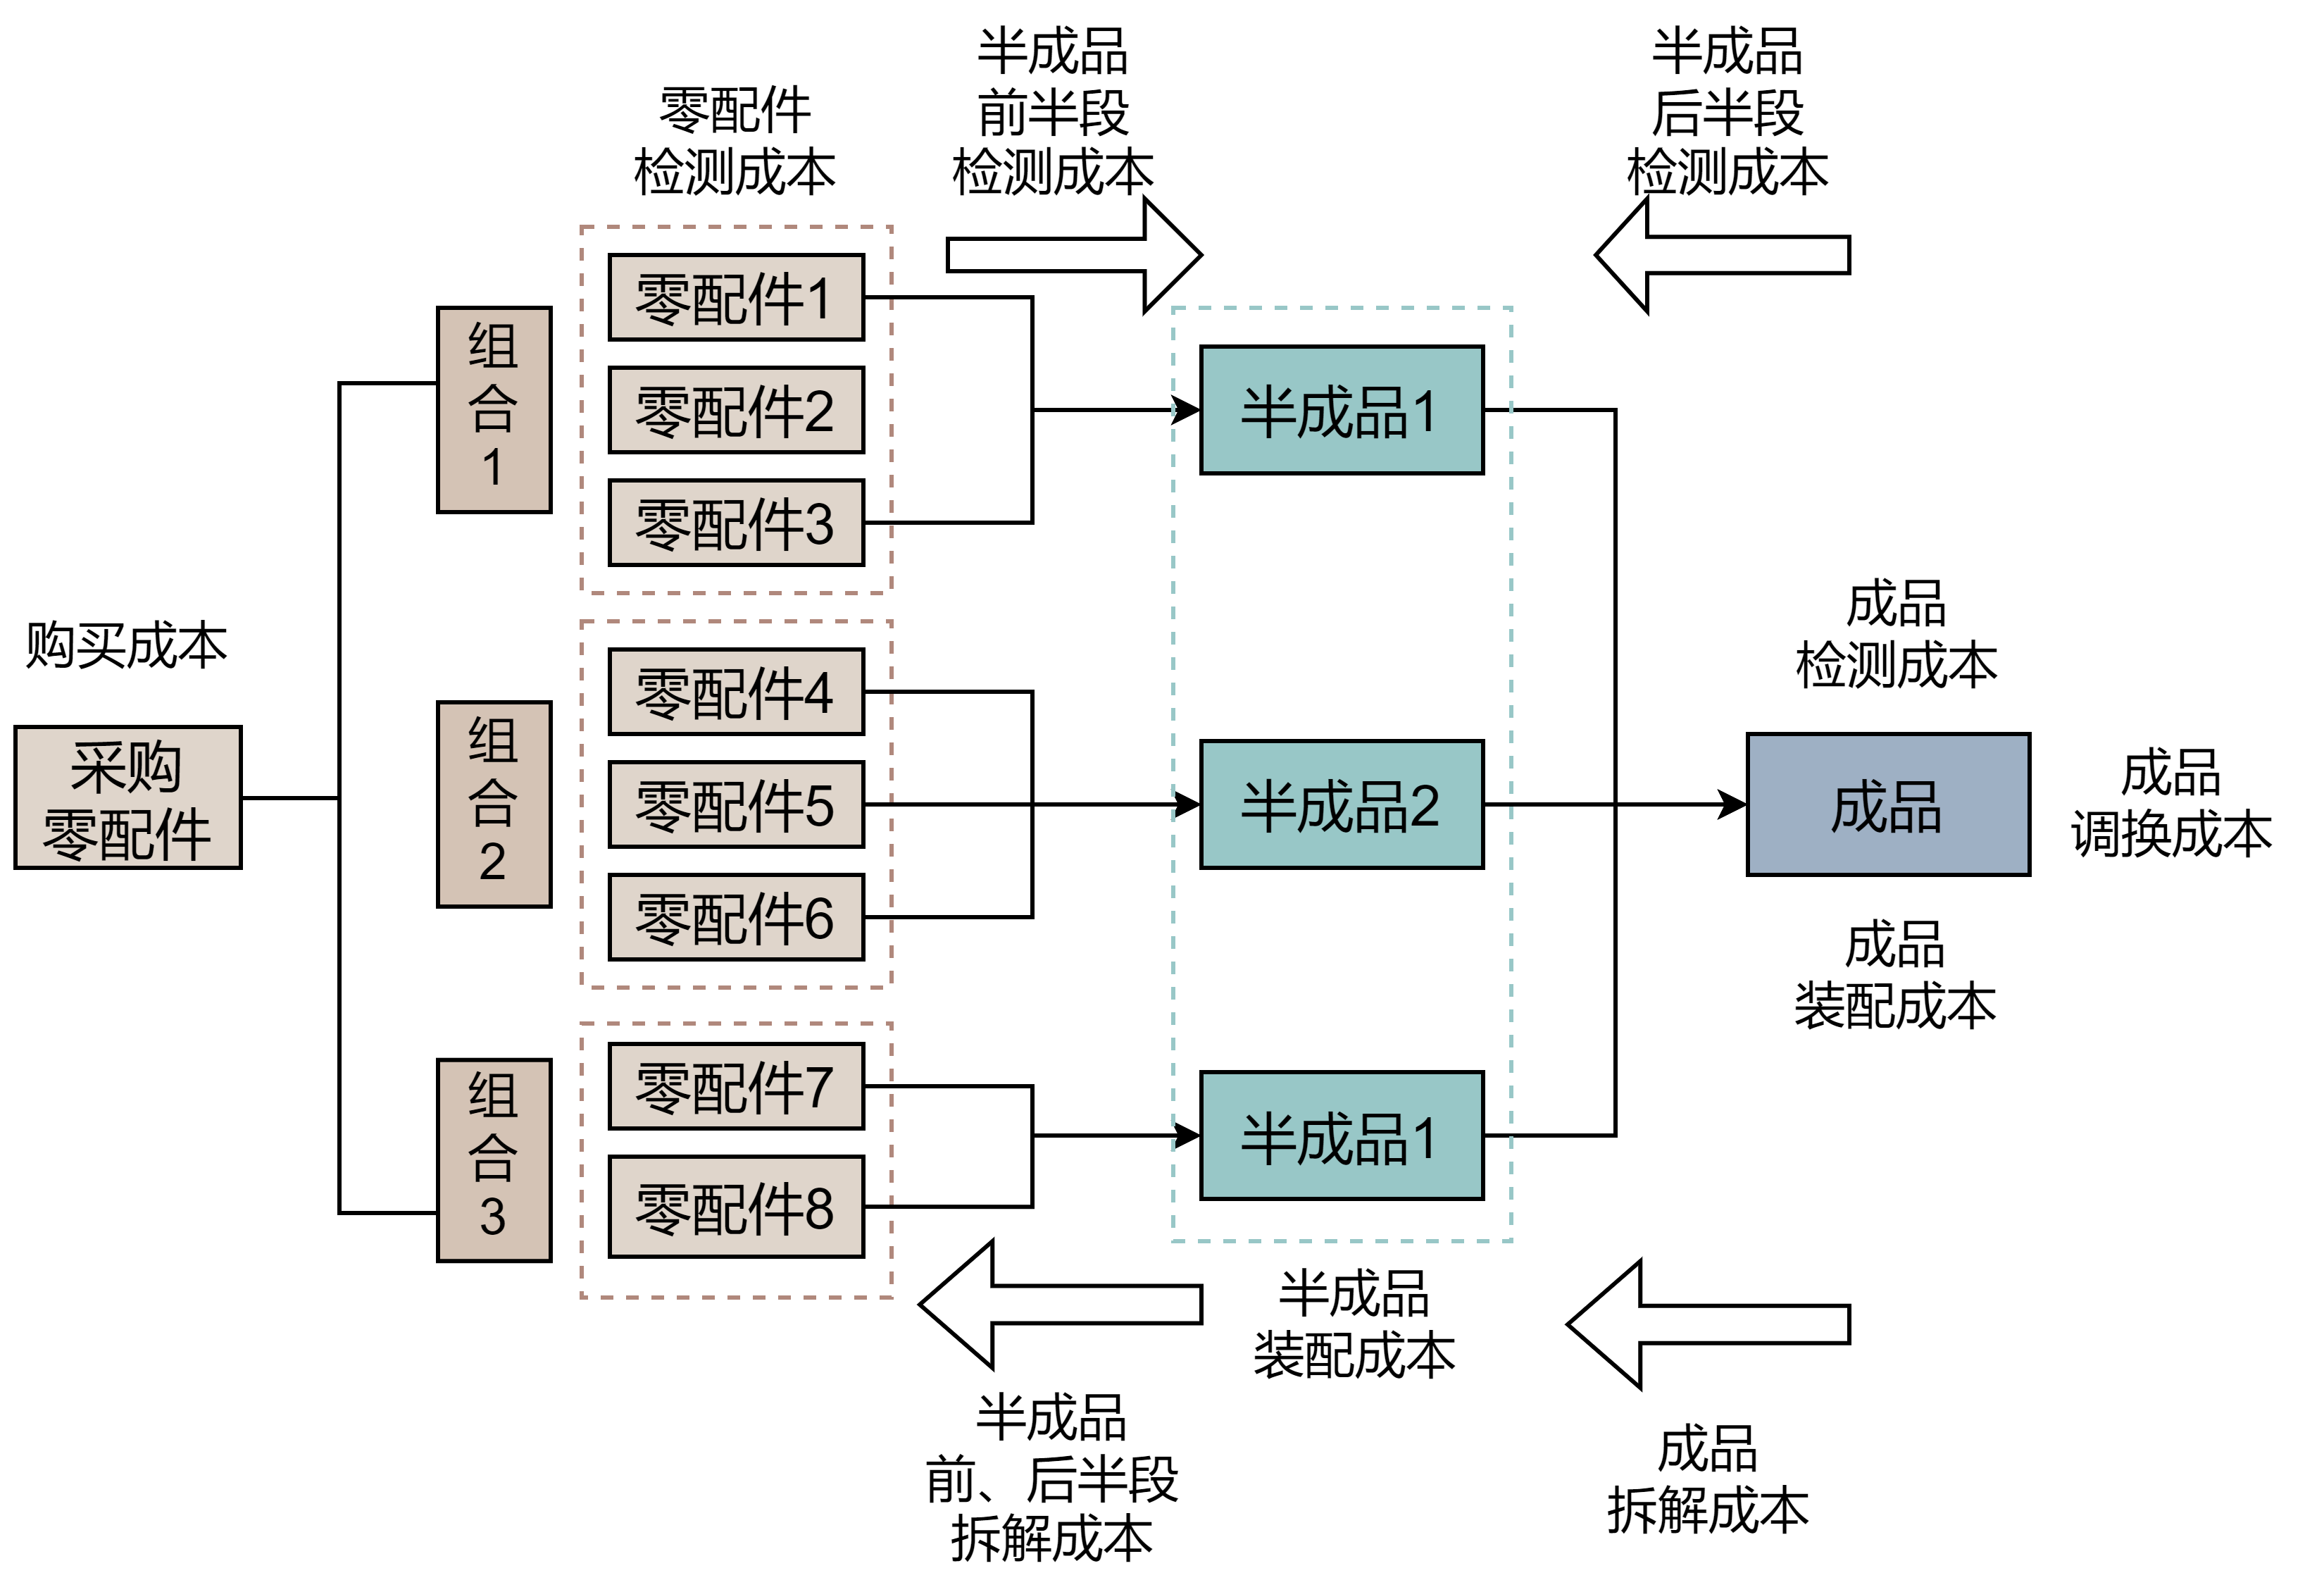
\includegraphics[width=.85\textwidth]{成} %图片的名称或者路径之中有空格会出问题  %.8用来调整图片大小
	\caption{成本构成}  
\end{figure}

\subsubsection*{(1) 购买成本}
由于假设所有零配件的数量均相等且等于单位1,故零配件的购买成本可表示为:
\begin{equation}
	c_0=\left(a_{01}+a_{02}+a_{03}\right) G_1+\left(a_{04}+a_{05}+a_{06}\right) G_2+\left(a_{07}+a_{031}\right) G_3
\end{equation}
其中,$a_{0i}$表示第$i$种零配件的购买单价。\begin{equation}
	q_1=\frac{\frac{\left(1-q_1\right)^2 \cdot\left(1-G_1\right) \cdot q_1}{\left(1-G_1 \cdot q_1\right)^2}+\frac{2\left(1-q_1\right) \cdot q_1^2 \cdot\left(1-G_1\right)^2}{\left(1-G_1 \cdot q_1\right)^2}+\frac{\left(1-G_1\right)^3-q_1^3}{\left(1-G_1 \cdot q_1\right)^2}}{1-\frac{\left(1-q_4\right) \cdot\left(1-q_1\right)^3}{\left(1-G_1 \cdot q_1\right)^2-G_1 \cdot q_1}}
\end{equation}

\subsubsection*{(2) 零配件检测成本}
为简化问题,设定以下0-1整数规划变量(0表示不检测,1表示检测):
\begin{equation*}
	\left\{\begin{array}{l}
		G_1: \text{零件1、2、3的检测决策变量}\\
		G_2: \text{零件4、5、6的检测决策变量}\\
		G_3:\text{零件7、8的检测决策变量}
	\end{array}\right.
\end{equation*}

经过检测后,各类零配件的数量更新为:
\begin{equation}
	\begin{aligned}
		&\left\{\begin{array}{l}
			n_1=n_2=n_3=\left(1-G_1 \cdot q_1\right) \\
			n_4=n_5=n_6=\left(1-G_2 \cdot q_2\right) \\
			n_7=n_8=\left(1-G_3 \cdot q_3\right)
		\end{array}\right. \\
		 \Rightarrow 
		 & \left\{\begin{array}{l}
			n_1=n_2=n_3=\left(1-q_1\right)+\left(1-G_1\right) \cdot q_1 \\
			n_4=n_5=n_6=\left(1-q_2\right)+\left(1-G_2\right) \cdot q_2 \\
			n_7=n_8=\left(1-q_3\right)+\left(1-G_3\right) \cdot q_3
		\end{array}\right.
	\end{aligned}
\end{equation}
其中,$q_1$,$q_2$,$q_3$分别表示零件1、2、3,零件4、5、6和零件7、8的次品率。进行是否检测决策后,将公式变形可得,$(1-q_1)$、$(1-q_2)$、$(1-q_3)$分别表示零件1、2、3,零件4、5、6和零件7、8的正品个数,$(1-G_1)\cdot q_1$表示相应的次品率次品个数。

由此可得,零配件的检测成本为:
\begin{equation}
	c_{21}=G_1 \cdot\left(a_{11}+a_{12}+a_{13}\right)+G_{22} \cdot\left(a_{14}+a_{15}+a_{16}\right)+G_3 \cdot\left(a_{17}+a_{18}\right)
\end{equation}
其中,$a_{1i}$表示第$i$个零件的检测成本。其他零配件的检测成本同理可得。

\subsubsection*{(3) 半成品装配成本}
半成品的装配原则与问题2相同,即“零配件耗尽”原则与“以频率估计概率”原则。

由于本问中零配件1、2、3的检测决策相同,因此半成品1的构成为:
\begin{equation}
	\left\{\begin{array}{l}
		\frac{\left(1-q_1\right)^3\left(1-q_4\right)}{\left(1-G_1 \cdot q_1\right)^2} \text{,正零件+正零件+正零件=正品半成品1}\\
		\frac{3\left(1-q_1\right)^2\left(1-G_1\right) \cdot q_1}{\left(1-G_1 \cdot q_1\right)^2} \text{,正零件+正零件+次零件=次品半成品1}\\
		\frac{3\left(1-q_1\right) \cdot q_1^2\left(1-G_1\right)^2}{\left(1-G_1 \cdot q_1\right)^2} \text{,正零件+次零件+次零件=次品半成品1}\\
		\frac{\left(1-G_1\right)^3 \cdot q_1^3}{\left(1-G_1 \cdot q_1\right)^2}\text{,次零件+次零件+次零件=次品半成品1}\\
		\frac{q_4 \cdot\left(1-q_1\right)^3}{\left(1-G_1 \cdot q_1\right)^2}\text{,正零件+正零件+正零件=次品半成品1}
	\end{array}\right.
\end{equation}
其中,$q_4$表示半成品1的次品率。半成品2的构成与半成品1类似,在此不做赘述。

零件7,8组装半成品3的组成:
\begin{equation}
	\left\{\begin{array}{l}
		\frac{\left(1-q_5\right)\left(1-q_2\right)^2}{1-G_2 \cdot q_2} \text{,正零件+正零件=正品半成品3}\\
		\frac{2\left(1-q_2\right) \cdot q_2}{1-G_2 \cdot q_2} \text{,正零件+次零件=次品半成品3}\\
		\frac{\left(1-G_2\right)^2 \cdot q_2^2}{1-G_2 \cdot q_2} \text{,次零件+次零件=次品半成品3}\\
		\frac{q_5 \cdot\left(1-q_2\right)^2}{1-G_2 \cdot q_2}\text{,正零件+正零件=次品半成品3}
	\end{array}\right.
\end{equation}

由此可得,半成品的装配成本为:
\begin{equation}
	c_{31}=\left(1-G_1 \cdot q_1\right) \cdot a_2+\left(1-G_2 \cdot q_2\right) \cdot a_2+\left(1-G_3 \cdot q_3\right) \cdot a_2
\end{equation}

\subsubsection*{(4) 半成品的前半段检测与拆解成本}
在本步骤中,由零配件装配成的半成品并不立刻开始加工成成品,而是等到零配件已尽可能地耗尽、不再有新的半成品生成时,才进入成品的加工操作。

设置以下0-1整数规划变量:
\begin{equation*}
	\left\{\begin{array}{l}
		H_1, H_2, H_3: \text{半成品1、2、3的前半段检测决策变量}\\
		I_1, I_2, I_3:\text{半成品1、2、3的前半段拆解决策变量}
	\end{array}\right.
\end{equation*}

因此,半成品前半段检测成本可表示为:
\begin{equation}
	c_{22_1}=H_1 \cdot\left(1-G_1 \cdot q_1\right) \cdot a_3+H_2 \cdot\left(1-G_2 \cdot q_2\right) \cdot a_3+H_3\cdot \left(1-G_3 \cdot q_3\right) \cdot a_3
\end{equation}
其中,$a_3$表示半成品的单次检测成本。

半成品前半段拆解成本可表示为:
\begin{equation}
	c_{41_1}=H_1 \cdot I_1 \cdot\left(1-G_1 \cdot q_1\right) \cdot a_4+H_2 \cdot I_2 \cdot\left(1-G_2 \cdot q_2\right) \cdot G_4+H_3 \cdot I_3\left(1-G_3 \cdot q_3\right) \cdot a_4
\end{equation}
其中,$a_4$表示半成品的单次拆解成本。

若$H_1\cdot I_1=1$,则表示对半成品进行检测且拆解,此时更新其组分零配件的次品率和数量后回到步骤一。同时设置阈值,防止循环次数过多,造成过程复杂。

以半成品1为例,其组分零配件次品率的更新公式为:
\begin{equation}
	q_1=\frac{\frac{\left(1-q_1\right)^2 \cdot\left(1-G_1\right) \cdot q_1}{\left(1-G_1 \cdot q_1\right)^2}+\frac{2\left(1-q_1\right) \cdot q_1^2 \cdot\left(1-G_1\right)^2}{\left(1-G_1 \cdot q_1\right)^2}+\frac{\left(1-G_1\right)^3-q_1^3}{\left(1-G_1 \cdot q_1\right)^2}}{1-\frac{\left(1-q_4\right) \cdot\left(1-q_1\right)^3}{\left(1-G_1 \cdot q_1\right)^2-G_1 \cdot q_1}}
\end{equation}

零配件数量更新公式为:
\begin{equation}
	n_1=n_2=n_3=N=\frac{1-G_1 \cdot q_1\left(1-q_4\right) \cdot\left(1-q_1\right)^3}{\left(1-G_1 \cdot q_1\right)^2}
\end{equation}
半成品2和半成品3的组分零配件的次品率和数量更新公式同理可得。需要注意的是,前一轮已被检测的零配件在后续轮中不再接受检测,以防止增加成本,可表示为:
\begin{equation}
	G_{i 1} \cdot G_{i 2} \neq 1
\end{equation}
其中,$G_{i1}$表示前一轮的零配件检测决策变量,$G_{i2}$表示后一轮的零配件检测决策变量。

由于整个决策过程是完全随机的,因此无法对半成品1、2、3的构成给出一个确定的数学表达式。为了后文讨论方便,将半成品1、2、3的构成分别化为:
\begin{equation}
	\left\{\begin{array}{l}
		A_1: \text{正零件+正零件+正零件=正品半成品1}\\
		A_2: \text{正零件+正零件+次零件=次品半成品1}\\
		A_3:\text{正零件+次零件+次零件=次品半成品1}\\
A_4:\text{次零件+次零件+次零件=次品半成品1}\\	
A_5:\text{正零件+正零件+正零件=次品半成品1}\end{array}\right.
\end{equation}
\begin{equation}
	\left\{\begin{array}{l}
		B_1: \text{正零件+正零件+正零件=正品半成品2}\\
		B_2: \text{正零件+正零件+次零件=次品半成品2}\\
		B_3:\text{正零件+次零件+次零件=次品半成品2}\\
		B_4:\text{次零件+次零件+次零件=次品半成品2}\\	
		B_5:\text{正零件+正零件+正零件=次品半成品2}\end{array}\right.
\end{equation}
\begin{equation}
	\left\{\begin{array}{l}
		O_1: \text{正零件+正零件=正品半成品3}\\
		O_2: \text{正零件++次零件=次品半成品3}\\
		O_3:\text{次零件+次零件=次品半成品3}\\
		O_4:\text{正零件+正零件=次品半成品3}
\end{array}\right.
\end{equation}
用$A$、$B$、$O$分别表示半成品1、2、3的总数,则:
\begin{equation}
	\left\{\begin{array}{l}
		A=A_1+A_2+A_3+A_4+A_5\\
		B=B_1+B_2+B_3+B_4+B_5\\
		O=O_1+O_2+O_3+O_4
	\end{array}\right.
\end{equation}

\subsubsection*{(5) 成品装配成本}
成品的装配与半成品遵循相同的原则,最终装配的成品总数由三种半成品中最少的数量决定。因此,需要找到$A$、$B$、$O$的最小值。

如果$A$是最小值,装配之后成品的构成应为:
\begin{equation}
	\left\{\begin{array}{l}
		\frac{\left(1-q_6\right) \cdot A_1 \cdot B_1 \cdot O_1}{B \cdot O} \text {, 正品 } \\
		A_2+A_3+A_4+A_5+\frac{q_6 \cdot A_1 \cdot B_1 \cdot O_1}{B \cdot O} \text {, 次品 } 
	\end{array}\right.
\end{equation}

如果$B$是最小值,装配之后成品的构成应为:
\begin{equation}
	\left\{\begin{array}{l}
		\frac{\left(1-q_6\right) \cdot A_1 \cdot B_1 \cdot O_1}{A \cdot O} \text {, 正品 } \\
		A_2+A_3+A_4+A_5+\frac{q_6 \cdot A_1 \cdot B_1 \cdot O_1}{A \cdot O} \text {, 次品 } 
	\end{array}\right.
\end{equation}

如果$O$是最小值,装配之后成品的构成应为:
\begin{equation}
	\left\{\begin{array}{l}
		\frac{\left(1-q_6\right) \cdot A_1 \cdot B_1 \cdot O_1}{A \cdot B} \text {, 正品 } \\
		A_2+A_3+A_4+A_5+\frac{q_6 \cdot A_1 \cdot B_1 \cdot O_1}{A \cdot B} \text {, 次品 } 
	\end{array}\right.
\end{equation}

最终的成品装配成本为:
\begin{equation}
	c_{32}=\min (A, B, O) \cdot a_5
\end{equation}
其中,$a_5$表示成品单次装配成本。
\subsubsection*{(6) 成品检测、拆解与调换成本}
设与成品的检测与拆解相关的0-1整数规划变量为:
\begin{equation}
	\left\{\begin{array}{l}
		J:\text{成品检测决策变量} \\
		K:\text{成品拆解决策变量}
	\end{array}\right.
\end{equation}

由此得到成品检测成本,可表示为:
\begin{equation}
	c_{23}=J \cdot \min (A, B, O) \cdot a_6
\end{equation}
其中,$a_6$表示成品单次检测成本。

为清晰阐述下述思路,不妨假定$A=min(A,B,O)$,则此时成品拆解成本可表示为:
\begin{equation}
	c_{42}=K \cdot\left(A-\frac{\left(1-q_6\right) \cdot A_1 \cdot B_1 \cdot O_1}{B \cdot O}\right)-a_7
\end{equation}
其中,$a_7$表示成品拆解成本。

成品调换成本可表示为:
\begin{equation}
	c_{5}=(1 - J) \cdot\left(A-\frac{\left(1-q_6\right) \cdot A_1 \cdot B_1 \cdot O_1}{B \cdot O}\right)-a_8
\end{equation}
其中,$a_8$表示调换损失成本。

\subsubsection*{(7) 半成品的后半段检测与拆解成本}
仍然假定$A=min(A,B,O)$。由前文,$K$表示成品拆解决策变量,如果$K=1$,则成品被拆解,拆解后$A_2$,$A_3$,$A_4$,$A_5$参与组成次成品的部分被归还回来,从而数量保持不变,即半成品的损失量为$\frac{\left(1-q_6\right) \cdot A_1 \cdot B_1 \cdot O_1}{B \cdot O}$,更新半成品中$A_1$的数量可表示为:
\begin{equation}
	A_1=A_1-\frac{\left(1-q_6\right) \cdot A_1 \cdot B_1 \cdot O_1}{B \cdot O}
\end{equation}

针对半成品的后半段检测过程,设置以下0-1整数规划变量:
\begin{equation*}
	\left\{\begin{array}{l}
		H_4, H_5, H_6: \text{半成品1、2、3的后半段检测决策变量}\\
		I_4, I_5, I_6:\text{半成品1、2、3的后半段拆解决策变量}
	\end{array}\right.
\end{equation*}

令$M=\frac{\left(1-q_6\right) \cdot A_1 \cdot B_1 \cdot O_1}{B \cdot O}$,则半成品后半段检测成本可表示为:
\begin{equation}
	c_{22_2}=H_4 \cdot(A-M) \cdot a_3+H_5 \cdot(B-M) \cdot a_3+H_6 \cdot(O-M) \cdot a_3
\end{equation}

半成品后半段拆解成本可表示为:
\begin{equation}
	c_{41_2}=H_4 \cdot I_4 \cdot(A-M) \cdot a_4+H_5 \cdot I_5 \cdot(B-M) \cdot a_4+H_6 \cdot I_6 \cdot(O-M) \cdot a_4
\end{equation}

若$H_i\cdot I_i=1$(i=4,5,6),则相应的半成品被拆解,进入第二轮的各个决策。为了避免模型过于复杂,在整体大循环上设置阈值$\gamma = 2$。

\subsubsection{销售额的计算}
成品的销售额可表示为:
\begin{equation}
	W=\frac{\left(1-q_6\right) \cdot A_1 \cdot B_1 \cdot O_1}{B \cdot O} \cdot a_9
\end{equation}
其中,$a_9$表示成品销售单价。

\subsubsection{最终利润的确定}
最终利润$\pi$可表示为:
\begin{equation}
	\pi=W-C
\end{equation}

\subsection{决策制定}

通过模型进行优化得到的最高利润为75.49,最优方案如下:
\textbf{1. 零配件检测及半成品前半段检测和拆解}

(1) 零配件1,2,3不检测,半成品1检测且拆解 $\rightarrow$ 零配件1,2,3检测,半成品1检测且拆解 $\rightarrow$ 零配件1,2,3不检测,半成品1检测且拆解 $\rightarrow$ 零配件1,2,3检测,半成品1不检测但拆解。

(2) 零配件4,5,6检测,半成品2检测不拆解。

(3) 零配件7,8 检测,半成品3不检测且不拆解。

\textbf{2. 成品检测与拆解及半成品后半段检测与拆解}
成品检测且拆解 $\rightarrow$ 次品半成品1检测但不拆解,次品半成品2不检测,次品半成品3检测且拆解 $\rightarrow$ 
次成品3的零件7,8进行检测合成半成品3后检测且拆解 $\rightarrow$ 零件7,8不检测半成品3不检测不拆解。

\textbf{3.由半成品到成品的成品装配}

成品检测。



\section{问题4模型的建立和求解}

题目要求使用问题1中所采用的抽样检测方法来确定零配件、半成品和成品的次品率,并应用到问题2和问题3中的各个情况中,从而重新制定生产决策。对此,结合前文提到的假设检验和整数规划等方法,建立以下模型,并按照问题1中的两种情形分情况讨论。

\subsection{次品率的确定}
首先,根据问题1中的公式几和公式几,$n_1$和$n_2$分别是关于$\hat{p_1}$和$\hat{p_2}$的函数。通过转换自变量和因变量的关系,可以将$\hat{p_1}$和$\hat{p_2}$表示成关于$n_1$和$n_2$的函数,即:

	\begin{equation}
	\begin{aligned}
			\hat{p_1} &\geqslant p_0 + 1.645 \times \sqrt{\frac{p_0 (1-p_0)}{n_1}} \\
			\Rightarrow \hat{p_1} &\geqslant 0.1 + \frac{0.4935}{\sqrt{n_1}}
		\end{aligned}
\end{equation}
\begin{equation}
	\begin{aligned}
			\hat{p_2} &\leqslant p_0 - 1.282 \times \sqrt{\frac{p_0 (1-p_0)}{n_2}} \\
			\Rightarrow \hat{p_2} &\leqslant 0.1 - \frac{0.3846}{\sqrt{n_2}}
		\end{aligned}
\end{equation}

因此,对于每一个预期进行的抽样检测次数,都可以在95\%和90\%的置信水平下分别得到一个样品次品率$\hat{p_1}$和$\hat{p_2}$。在完成抽样检测后,若样品次品率高于$\hat{p_1}$,则有95\%的把握认为零配件次品率超过标称值,并予以拒收;若样品次品率低于$\hat{p_2}$,则有90\%的把握认为零配件次品率不超过标称值,并予以接收。

在本问题中,为了简化模型,作出以下假设:如果通过假设检验已经验证了预期值是正确的,则使用预期次品率代替零配件总体的实际次品率。同时,这种基于假设检验的抽样检测方法也被应用于半成品和成品的检测过程中,将该种基于假设检验的抽样检测方法同时应用到对零配件、半成品和成品的检测上,并认为在相同情形下,三种检测的预期和结果是一致的,即零配件次品率=半成品次品率=成品次品率。

根据检验统计量的确定过程,假设检验是在大样本的条件下进行的。而根据统计学知识,大样本指的是样本数量至少为30,以避免出现较大的随机误差。同时,为降低企业的检测成本,样本数量不应过大。综合考虑以上因素,在此问题中,选择抽样数量$n_1=n_2=n=100$,并由此得出$\hat{p_1}=15\%$、$\hat{p_2}=6\%$,分别代表情形(1)和情形(2)中,在95\%和90\%置信水平下的次品率。相关函数关系与其在图像中的位置如下图所示:

\begin{figure}[htbp]
	\centering
	\begin{subfigure}[t]{0.49\textwidth}
		\centering
		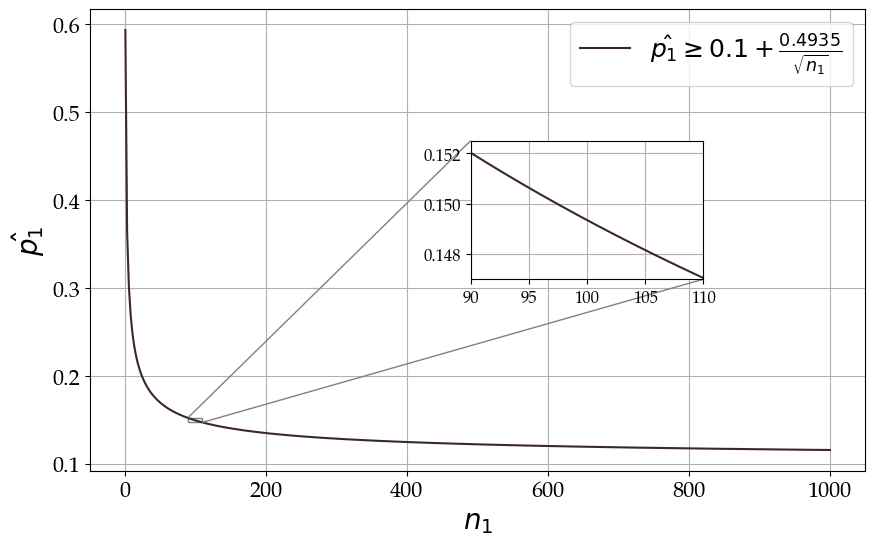
\includegraphics[width=\textwidth]{951}
		\caption{$\hat{p_1}$和$n_1$的函数关系}
		\label{fig:sub1}
	\end{subfigure}
	\hfill
	\begin{subfigure}[t]{0.49\textwidth}
		\centering
		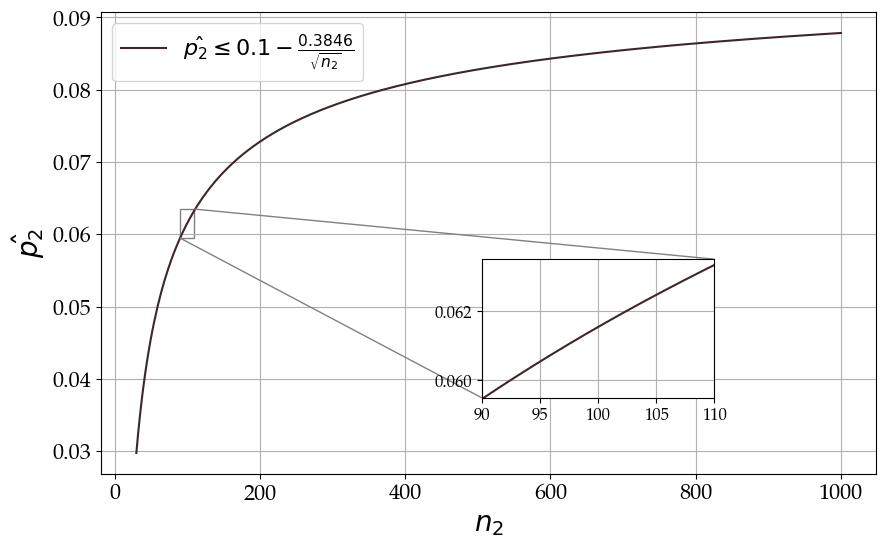
\includegraphics[width=\textwidth]{901}
		\caption{$\hat{p_2}$和$n_2$的函数关系}
		\label{fig:sub2}
	\end{subfigure}
	\caption{两个函数关系}
	\label{fig:both}
\end{figure}

\subsection{决策方案的制定}

\subsubsection{问题2中的决策方案}
\subsubsection*{情形(1)}
当置信水平为95\%时,将次品率$\hat{p_1}=15\%$代入问题2中的模型求解,并保持其他条件不变。综合考虑零件检测、成品组装、成品检测、不合格品拆解及调换等步骤,通过整数规划和蒙特卡洛模拟的方法建立利润最大化模型,并进行优化,从而得出最优的决策方案。具体的的决策方案如下表所示。

\begin{table}[htbp]
		\centering
	\caption{情形(1)中问题2的决策方案}
	\scalebox{0.62}{
	\begin{tabular}{c|c|cccc|cccc|cccc}
		\toprule[1.5pt]
		\multirow{2}{*}{情况} & \multirow{2}{*}{最终利润} & \multicolumn{4}{c|}{第一轮决策}                                                                                                                                                                                  & \multicolumn{4}{c|}{第二轮决策}                                                                                                                                                                                  & \multicolumn{4}{c}{第三轮决策}                                                                                                                                                                                   \\ \cline{3-14} 
		&                       & \begin{tabular}[c]{@{}c@{}}零配件1\\ 检测\end{tabular} & \begin{tabular}[c]{@{}c@{}}零配件2\\ 检测\end{tabular} & \begin{tabular}[c]{@{}c@{}}成品\\ 检测\end{tabular} & \begin{tabular}[c]{@{}c@{}}不合格品\\ 拆解\end{tabular} & \begin{tabular}[c]{@{}c@{}}零配件1\\ 检测\end{tabular} & \begin{tabular}[c]{@{}c@{}}零配件2\\ 检测\end{tabular} & \begin{tabular}[c]{@{}c@{}}成品\\ 检测\end{tabular} & \begin{tabular}[c]{@{}c@{}}不合格品\\ 拆解\end{tabular} & \begin{tabular}[c]{@{}c@{}}零配件1\\ 检测\end{tabular} & \begin{tabular}[c]{@{}c@{}}零配件2\\ 检测\end{tabular} & \begin{tabular}[c]{@{}c@{}}成品\\ 检测\end{tabular} & \begin{tabular}[c]{@{}c@{}}不合格品\\ 拆解\end{tabular} \\ \hline
		1                   & 10.56n                 & 是                                                 & 是                                                 & 否                                               & 是                                                 & 否                                                 & 否                                                 & 否                                               & 是                                                 & 否                                                 & 否                                                 & 否                                               & 否                                                 \\
		2                   & 10.56n                 & 是                                                 & 是                                                 & 否                                               & 是                                                 & 否                                                 & 否                                                 & 否                                               & 是                                                 & 否                                                 & 否                                                 & 否                                               & 否                                                 \\
		3                   & 8.85n                  & 是                                                 & 是                                                 & 是                                               & 是                                                 & 否                                                 & 否                                                 & 是                                               & 是                                                 & 否                                                 & 否                                                 & 是                                               & 否                                                 \\
		4                   & 12.98n                 & 是                                                 & 是                                                 & 是                                               & 是                                                 & 否                                                 & 否                                                 & 是                                               & 是                                                 & 否                                                 & 否                                                 & 是                                               & 否                                                 \\
		5                   & 7.94n                  & 否                                                 & 否                                                 & 是                                               & 是                                                 & 是                                                 & 是                                                 & 是                                               & 是                                                 & 否                                                 & 否                                                 & 否                                               & 否                                                 \\
		6                   & 3.39n                  & 否                                                 & 否                                                 & 是                                               & 否                                                 & -                                                 & -                                                 & -                                               & -                                                 & -                                                 & -                                                 & -                                               & -                                                 \\ \bottomrule[1.5pt]
	\end{tabular}
}
\end{table}

\subsubsection*{情形(2)}
同理,当置信水平为90\%时,将次品率$\hat{p_2}=6\%$代入问题2中的模型求解,同时保持其他条件不变。同样地,通过上述方法进行优化后,得到的最优的决策方案如下表所示:
\begin{table}[htbp]
			\centering
	\caption{情形(2)在问题2中的决策方案}
	\scalebox{0.62}{
	\begin{tabular}{c|c|cccc|cccc|cccc}
		\toprule[1.5pt]
		\multirow{2}{*}{情况} & \multirow{2}{*}{最终利润} & \multicolumn{4}{c|}{第一轮决策}                                                                                                                                                                                  & \multicolumn{4}{c|}{第二轮决策}                                                                                                                                                                                  & \multicolumn{4}{c}{第三轮决策}                                                                                                                                                                                   \\ \cline{3-14} 
		&                       & \begin{tabular}[c]{@{}c@{}}零配件1\\ 检测\end{tabular} & \begin{tabular}[c]{@{}c@{}}零配件2\\ 检测\end{tabular} & \begin{tabular}[c]{@{}c@{}}成品\\ 检测\end{tabular} & \begin{tabular}[c]{@{}c@{}}不合格品\\ 拆解\end{tabular} & \begin{tabular}[c]{@{}c@{}}零配件1\\ 检测\end{tabular} & \begin{tabular}[c]{@{}c@{}}零配件2\\ 检测\end{tabular} & \begin{tabular}[c]{@{}c@{}}成品\\ 检测\end{tabular} & \begin{tabular}[c]{@{}c@{}}不合格品\\ 拆解\end{tabular} & \begin{tabular}[c]{@{}c@{}}零配件1\\ 检测\end{tabular} & \begin{tabular}[c]{@{}c@{}}零配件2\\ 检测\end{tabular} & \begin{tabular}[c]{@{}c@{}}成品\\ 检测\end{tabular} & \begin{tabular}[c]{@{}c@{}}不合格品\\ 拆解\end{tabular} \\ \hline
		1                   & 20.38n                & 否                                                 & 否                                                 & 否                                               & 是                                                 & 是                                                 & 是                                                 & 否                                               & 是                                                 & 否                                                 & 否                                                 & 否                                               & 否                                                 \\
		2                   & 20.38n                & 否                                                 & 否                                                 & 否                                               & 是                                                 & 是                                                 & 是                                                 & 否                                               & 是                                                 & 否                                                 & 否                                                 & 否                                               & 否                                                 \\
		3                   & 18.26n                & 否                                                 & 否                                                 & 是                                               & 是                                                 & 是                                                 & 是                                                 & 是                                               & 是                                                 & 否                                                 & 否                                                 & 否                                               & 否                                                 \\
		4                   & 19.88n                & 否                                                 & 否                                                 & 是                                               & 是                                                 & 是                                                 & 是                                                 & 是                                               & 是                                                 & 否                                                 & 否                                                 & 否                                               & 否                                                 \\
		5                   & 19.06n                & 否                                                 & 否                                                 & 否                                               & 是                                                 & 是                                                 & 是                                                 & 是                                               & 是                                                 & 否                                                 & 否                                                 & 否                                               & 否                                                 \\
		6                   & 16.82n                & 否                                                 & 否                                                 & 否                                               & 否                                                 & -                                                 & -                                                 & -                                               & -                                                 & -                                                 & -                                                 & -                                               & -                                                 \\ \bottomrule[1.5pt]
	\end{tabular}
}
\end{table}

\subsubsection{问题3中的决策方案}
\subsubsection*{情形(1)}
当置信水平为95\%时,将次品率$\hat{p_1}=15\%$代入问题3中的模型求解,并保持其他条件不变,得到的最高利润为71.15,最优决策方案为:

\textbf{1. 零配件检测及半成品前半段检测和拆解}

(1)零配件1,2,3不检测,半成品1检测且拆解 $\rightarrow$ 零配件1,2,3检测,半成品1检测且拆解 $\rightarrow$ 零配件1,2,3不检测,半成品1检测且拆解 $\rightarrow$ 零配件1,2,3检测。

(2)零配件4,5,6检测,半成品2检测但不拆解。

(3)零配件7,8不检测,半成品3不检测。

\textbf{2.成品检测和拆解及半成品后半段检测和拆解}

成品检测且拆解 $\rightarrow$ 次品半成品1检测且拆解,次品半成品2不检测且不拆解,次品半成品3检测但不拆解 $\rightarrow$ 零配件1,2,3不检测,半成品1不拆解。

\textbf{3.由半成品到成品的成品装配}

成品检测且拆解 $\rightarrow$ 半成品3检测 $\rightarrow$ 成品检测。

\subsubsection*{情形(2)}
同理,当置信水平为90\%时,将次品率$\hat{p_1}=6\%$代入问题3中的模型求解,并保持其他条件不变,得到的最高利润为120.53,最优决策方案为:

\textbf{1. 零配件检测及半成品前半段检测和拆解}

(1)零配件1,2,3不检测,半成品1检测且拆解 $\rightarrow$ 零配件1,2,3检测,半成品1检测且拆解 $\rightarrow$ 零配件1,2,3不检测。

(2) 零配件4,5,6不检测,半成品2检测且拆解 $\rightarrow$ 零配件4,5,6检测,半成品2不检测。

(3) 零配件7,8不检测,半成品3检测且拆解 $\rightarrow$ 零配件7,8不检测,半成品3检测且拆解 $\rightarrow$ 零配件7,8检测,半成品3检测且拆解 $\rightarrow$ 零配件7,8不检测,半成品3检测但不拆解。

\textbf{2. 成品检测与拆解}

成品不检测且不拆解。

\section{模型的评价与推广}

\subsection{模型的优点}
1. 本文的模型是在合理假设的基础上,经过严格的数学推导过程建立的,事实是符合实际的,逻辑是能够自洽的。

2. 问题2建立的数学模型可以得到在各种决策情况下的最优值,结果具有极高的准确性。

3. 问题3建立的数学模型使用了分段计算成本以及零配件最大化利用策略,大大简化了数学建模的过程,提高了模型的拟合效果。

\subsection{模型的缺点}
1. 问题3中建立的数学模型虽然已经经过了简化,但仍然非常复杂,导致求解的难度极大。

2. 由于模型对实际情况进行了一定的简化,因此提出的方案始终存在一些误差。

\subsection{模型的推广}
1. 问题2和3中建立的数学模型都可应用于企业的生产决策制定过程,帮助企业扩大收益。

2. 进一步变化次品率可获得应用更广泛的生产决策方案。

%最后采用的是外面导入bib文件形式
\bibliographystyle{plain}
\bibliography{ref.bib}

\newpage
%附录
\appendix
\section*{附录}
\section{支撑文件列表}
\begin{center}
	\begin{tabular}{cc}
		\toprule[1.5pt]
		\makebox[0.2\textwidth][c]{题号}	&  \makebox[0.3\textwidth][c]{文件名称} \\
		\midrule[1pt]
		问题1	    	& 第一问求解.py   \\ 
	问题2    	& 第二问求解.py  \\ 
		问题3	    	& 第三问求解.py \\ 
		问题4	    	& 第四问求解.py  \\  

		\bottomrule[1.5pt]
	\end{tabular}
\end{center}
\section{问题1求解代码}
\begin{lstlisting}[language=python]
import numpy as np
import matplotlib.pyplot as plt
import matplotlib as mpl
from mpl_toolkits.axes_grid1.inset_locator import inset_axes, mark_inset

mpl.rcParams['font.family'] = 'Palatino Linotype'

def calculate_n(p):
return (0.4935 / (p - 0.1)) ** 2

# 给定 p 值求对应的 n 值
p = 0.15
n = calculate_n(p)
print(f'p = {p}, n = {n}')

p_values = np.linspace(0.11, 1, 400)
n_values = calculate_n(p_values)

# 主图设置
fig, ax = plt.subplots(figsize=(10, 6))
ax.plot(p_values, n_values, label=r'${n_1} \geq \left( \frac{0.4935}{\hat{p_1} - 0.1} \right)^2$', color='#708194')

ax.set_xlabel(r'$\hat{p_1}$', fontsize=20)
ax.set_ylabel('$n_1$', fontsize=20)
ax.tick_params(axis='x', labelsize=16)
ax.tick_params(axis='y', labelsize=16)
ax.legend(fontsize=18)
ax.grid(True)

# 创建放大区域
axins = inset_axes(ax, width="50%", height="50%", loc='lower right',
bbox_to_anchor=(0.2, 0.35, 0.7, 0.7),
bbox_transform=ax.transAxes)

# 在放大区域中绘制相同的函数
x_zoomed = np.linspace(0.11, 0.20, 400)
y_zoomed = calculate_n(x_zoomed)
axins.plot(x_zoomed, y_zoomed, color='#8ea0aa')
axins.grid(True)

# 设置放大区域的x轴和y轴限制
axins.set_xlim(0.14, 0.16)
axins.set_ylim(70, 150)
axins.tick_params(axis='x', labelsize=14)
axins.tick_params(axis='y', labelsize=14)

# 添加放大区域和主图之间的连接线
mark_inset(ax, axins, loc1=2, loc2=4, fc="none", ec="0.5")

plt.show()

def calculate_n(p):
return (0.3846 / (0.1 - p)) ** 2

p_values = np.linspace(0, 0.09, 400)
n_values = calculate_n(p_values)

# 给定p值求对应的n值
p = 0.06
n = calculate_n(p)
print(f'p = {p}, n = {n}')

# 主图设置
fig, ax = plt.subplots(figsize=(10, 6))
ax.plot(p_values, n_values, label=r'${n_2} \geq \left( \frac{0.3846}{0.1 - \hat{p_2}} \right)^2$', color='#708194')

ax.set_xlabel(r'$\hat{p_2}$', fontsize=20)
ax.set_ylabel('$n_2$', fontsize=20)
ax.tick_params(axis='x', labelsize=16)
ax.tick_params(axis='y', labelsize=16)
ax.legend(fontsize=18)
ax.grid(True)

# 创建放大区域,位置和大小通过参数调整
axins = inset_axes(ax, width="50%", height="50%", loc='lower right',
bbox_to_anchor=(-0.15, 0.3, 0.7, 0.7),
bbox_transform=ax.transAxes)

# 在放大区域中绘制相同的函数
x_zoomed = np.linspace(0, 0.09, 400)
y_zoomed = calculate_n(x_zoomed)
axins.plot(x_zoomed, y_zoomed, color='#8ea0aa')
axins.grid(True)

# 设置放大区域的x轴和y轴限制
axins.set_xlim(0.05, 0.07)
axins.set_ylim(50, 175)
axins.tick_params(axis='x', labelsize=14)
axins.tick_params(axis='y', labelsize=14)

# 添加放大区域和主图之间的连接线
mark_inset(ax, axins, loc1=1, loc2=3, fc="none", ec="0.5")

plt.show()
 \end{lstlisting}
 
 \section{问题2求解代码}
 \begin{lstlisting}[language=python]
 	import random
 	import math
 	
 	def profit(n1, n2, q1, q2, q3, a1, a2, a3, a4, a5, a6, a7, a8, a9, D1, D2, E, F):
 	"""
 	计算利润总和、成品数量及更新后的次品率
 	"""
 	# 零件检测成本
 	c21 = n1 * D1 * a2 + n2 * D2 * a4
 	
 	# 更新零件数量,考虑是否检测
 	n1 = (1 - D1 * q1) * n1
 	n2 = (1 - D2 * q2) * n2
 	
 	if n1 >= n2:  # 如果零件1数量多于零件2
 	c22 = n2 * E * a6  # 成品检测成本
 	c2 = c22 + c21     # 总检测成本
 	c3 = n2 * a5       # 装配成本
 	c4 = F * (n2 - (1 - q3) * (1 - q2) * n2 * (1 - q1) / (1 - D1 * q1)) * a9  # 拆解费用
 	c5 = (1 - E) * (n2 - (1 - q3) * (1 - q2) * n2 * (1 - q1) / (1 - D1 * q1)) * a8  # 调换成本
 	w = (1 - q3) * (1 - q2) * n2 * (1 - q1) / (1 - D1 * q1) * a7  # 销售额
 	A = c2 + c3 + c4 + c5   # 成本总和
 	pi = w - A              # 利润总和
 	
 	# 更新次品率
 	N = n2 - (1 - q3) * (1 - q2) * n2 * (1 - q1) / (1 - D1 * q1)
 	q1_new = ((1 - q2) * n2 * (1 - D1) * q1 / (1 - D1 * q1) +
 	(1 - D2) * q2 * n2 * (1 - D1) * q1 * (1 - D1 * q1)) / N
 	q2_new = ((1 - D2) * q2 * n2 * (1 - q1) / (1 - D1 * q1) +
 	(1 - D2) * q2 * n2 * (1 - D1) * q1 / (1 - D1 * q1)) / N
 	else:  # 如果零件1数量少于零件2
 	c22 = n1 * E * a6  # 成品检测成本
 	c2 = c22 + c21     # 总检测成本
 	c3 = n1 * a5       # 装配成本
 	c4 = F * (n1 - (1 - q3) * (1 - q1) * n1 * (1 - q2) / (1 - D2 * q2)) * a9  # 拆解费用
 	c5 = (1 - E) * (n1 - (1 - q3) * (1 - q1) * n1 * (1 - q2) / (1 - D2 * q2)) * a8  # 调换成本
 	w = (1 - q3) * (1 - q1) * n1 * (1 - q2) / (1 - D2 * q2) * a7  # 销售额
 	A = c2 + c3 + c4 + c5   # 成本总和
 	pi = w - A              # 利润总和
 	
 	# 更新次品率
 	N = n1 - (1 - q3) * (1 - q1) * n1 * (1 - q2) / (1 - D2 * q2)
 	q2_new = ((1 - q1) * n1 * (1 - D2) * q2 / (1 - D2 * q2) +
 	(1 - D1) * q1 * n1 * (1 - D2) * q2 * (1 - D2 * q2)) / N
 	q1_new = ((1 - D1) * q1 * n1 * (1 - q2) / (1 - D2 * q2) +
 	(1 - D1) * q1 * n1 * (1 - D2) * q2 / (1 - D2 * q2)) / N
 	
 	return pi, N, q1_new, q2_new
 	
 	q1,q2,q3,a1,a2,a3,a4,a5,a6,a7,a8,a9=0.1,0.1,0.1,4,2,18,3,6,3,56,6,5
 	#q1,q2,q3,a1,a2,a3,a4,a5,a6,a7,a8,a9=0.2,0.2,0.2,4,2,18,3,6,3,56,6,5
 	#q1,q2,q3,a1,a2,a3,a4,a5,a6,a7,a8,a9=0.1,0.1,0.1,4,2,18,3,6,3,56,30,5
 	#q1,q2,q3,a1,a2,a3,a4,a5,a6,a7,a8,a9=0.2,0.2,0.2,4,1,18,1,6,2,56,30,5
 	#q1,q2,q3,a1,a2,a3,a4,a5,a6,a7,a8,a9=0.1,0.2,0.1,4,8,18,1,6,2,56,10,5
 	#q1,q2,q3,a1,a2,a3,a4,a5,a6,a7,a8,a9=0.05,0.05,0.05,4,2,18,3,6,3,56,10,40
 	
 	# 主程序
 	max_pi = 0
 	lst_max = []
 	lst_pi = []  # 存储1000个利润
 	lst_decision = []  # 存储决策过程
 	
 	for _ in range(1000):
 	n1 = n2 = 1  # 初始零件数量
 	pi = 0
 	decisions = []  # 记录每次的决策状态
 	
 	# 随机选择决策
 	D1 = random.choice([0, 1])
 	D2 = random.choice([0, 1])
 	E = random.choice([0, 1])
 	F = random.choice([0, 1])
 	decisions.extend([D1, D2, E, F])
 	
 	# 计算利润、数量和次品率
 	pi1, N, q1_new, q2_new = profit(n1, n2, q1, q2, q3, a1, a2, a3, a4, a5, a6, a7, a8, a9, D1, D2, E, F)
 	
 	n = 0
 	while F == 1:
 	n1 = n2 = N  # 更新数量
 	D1 = random.choice([0, 1])
 	D2 = random.choice([0, 1])
 	E = random.choice([0, 1])
 	F = random.choice([0, 1])
 	
 	# 计算新一轮利润
 	pi2, N, q1_new, q2_new = profit(n1, n2, q1_new, q2_new, q3, a1, a2, a3, a4, a5, a6, a7, a8, a9, D1, D2, E, F)
 	
 	if pi2 > 0:
 	decisions.extend([D1, D2, E, F])
 	pi1 += pi2
 	else:
 	break
 	
 	if n > 3:
 	break
 	n += 1
 	
 	# 记录每次模拟的结果
 	lst_pi.append(pi1)
 	lst_decision.append(decisions)
 	
 	# 更新最大利润
 	if max_pi < pi1:
 	max_pi = pi1
 	lst_max = decisions
 	
 	# 检查是否有更好的决策方案
 	for i in range(1000):
 	if abs(max_pi - lst_pi[i]) / max_pi < 0.0025 and len(lst_max) > len(lst_decision[i]):
 	max_pi = lst_pi[i]
 	lst_max = lst_decision[i]
 	
 	# 打印结果
 	print(max_pi)
 	print(lst_max)
 	
 \end{lstlisting}
 
 \section{问题3求解代码}
  \begin{lstlisting}[language=python]
 	import random
 	number=0
 	lst11=[]#存储决策
 	lst12=[]#存储利润
 	lst141,lst151=[],[]
 	for i in range(10000):
 	lst131=[]
 	
 	# try:
 	def three_1(n1,q1,G1,H1,I1,q4=0.1):
 	#print(n1)
 	c21=G1*(n1+n1+2*n1) #零件检测成本
 	c31=(1-G1*q1)*8*n1 #半成品装配成本
 	c22_1=H1*(1-G1*q1)*4*n1 #半成品检测成本
 	c41_1=H1*I1*(1-G1*q1-((1-q1)**3)*(1-q4)/(1-G1*q1)**2)*6*n1 #半成品拆解成本
 	AA1=(1-q1)**3*(1-q4)/(1-G1*q1)**2*n1
 	AA2=q4*(1-q1)**3/(1-G1*q1)**2*n1
 	AA3=3*(1-q1)**2*(1-G1)*q1/(1-G1*q1)**2*n1
 	AA4=3*(1-q1)*((1-G1)*q1)**2/(1-G1*q1)**2*n1
 	AA5=(1-G1)**3*q1**3/(1-G1*q1)**2
 	N=(1-G1*q1-(1-q4)*((1-q1)**3)/(1-G1*q1)**2)*n1 #更新数量
 	# print(N)
 	# print(q1)
 	q=((((1-q1)**2)*(1-G1)*q1/(1-G1*q1)**2)+(1-q1)*(((1-G1)*q1)**2)/((1-G1*q1)**2)*2+(1-q1)*(((1-G1)*q1)**2)/(1-G1*q1)**2)/N #更新次品率
 	
 	return c21,c31,c22_1,c41_1,N,q,AA1,AA2,AA3,AA4,AA5
 	
 	def two_1(n1,q1,G1,H1,I1,q4=0.1):
 	c21=G1*3*n1 #零件检测成本
 	c31=(1-G1*q1)*8*n1 #半成品装配成本
 	c22_1=H1*(1-G1*q1)*4*n1 #半成品检测成本
 	c41_1=H1*I1*(1-G1*q1-(1-q4)*(1-q1)**2/(1-G1*q1))*6*n1#半成品拆解成本
 	CC1=(1-q4)*(1-q1)**2/(1-G1*q1)*n1
 	CC2=2*(1-q1)*q1*n1/(1-G1*q1)
 	CC3=((1-G1)*q1)**2/(1-G1*q1)*n1
 	CC4=q4*(1-q1)**2/(1-G1*q1)*n1
 	N=(1-G1*q1-(1-q4)*((1-q1)**3)/(1-G1*q1)**2)*n1 #更新数量
 	q=((1-q1)*q1*n1/(1-G1*q1)+((1-G1)*q1)**2/(1-G1*q1))/N#更新次品率
 	return c21,c31,c22_1,c41_1,N,q,CC1,CC2,CC3,CC4
 	A1,A2,A3,A4,A5=0,0,0,0,0 #用来记录半成品1的状态
 	B1,B2,B3,B4,B5=0,0,0,0,0# 用来记录半成品2的状态
 	O1,O2,O3,O4=0,0,0,0#用来记录半成品3的状态
 	M1,M2,M3=100,100,100 #存储零件数量
 	V1,V2,V3=0.1,0.1,0.1 #储存次品率
 	W=0
 	S=0
 	pi2=0
 	
 	A=A1+A2+A3+A4+A5
 	B=B1+B2+B3+B4+B5
 	O=O1+O2+O3+O4
 	
 	
 	lst1=[]#列表记录生成半成品1的决策过程
 	G1=random.choice([0,1])
 	H1=random.choice([0,1])
 	I1=random.choice([0,1])
 	lst1.append(G1)
 	lst1.append(H1)
 	lst1.append(I1)
 	c21,c31,c22_1,c41_1,N,q,A1,A2,A3,A4,A5=three_1(M1,V1,G1,H1,I1,q4=0.1)
 	S+=c21+c31+c22_1+c41_1
 	A2*=(1-H1)
 	A3*=(1-H1)
 	A4*=(1-H1)
 	A5*=(1-H1)
 	n=0#设置n来指示阈值
 	while H1*I1==1:
 	if n>2:
 	break
 	else:
 	if G1==1: #第一轮检测零件后第二轮不应该检测
 	G1=0
 	else:
 	G1=random.choice([0,1])
 	H1=random.choice([0,1])
 	I1=random.choice([0,1])
 	lst1.append(G1)
 	lst1.append(H1)
 	lst1.append(I1)
 	c21,c31,c22_1,c41_1,N,q,AA1,AA2,AA3,AA4,AA5=three_1(N,q,G1,H1,I1,q4=0.1)
 	S+=c21+c31+c22_1+c41_1
 	A1+=AA1
 	A2,A3,A4,A5=AA2,AA3,AA4,AA5
 	#print(lst1)
 	lst2=[]#列表记录生成半成品2的决策过程
 	G2=random.choice([0,1])
 	H2=random.choice([0,1])
 	I2=random.choice([0,1])
 	lst2.append(G2)
 	lst2.append(H2)
 	lst2.append(I2)
 	c21,c31,c22_1,c41_1,N,q,B1,B2,B3,B4,B5=three_1(M2,V2,G2,H2,I2,q4=0.1)
 	S+=c21+c31+c22_1+c41_1
 	B2*=(1-H2)
 	B3*=(1-H2)
 	B4*=(1-H2)
 	B5*=(1-H2)
 	n=0#设置n来指示阈值
 	while H2*I2==1:
 	if n>2:
 	break
 	if G2==1: #第一轮检测零件后第二轮不应该检测
 	G2=0
 	else:
 	G2=random.choice([0,1])
 	H2=random.choice([0,1])
 	I2=random.choice([0,1])
 	lst2.append(G2)
 	lst2.append(H2)
 	lst2.append(I2)
 	c21,c31,c22_1,c41_1,N,q,AA1,AA2,AA3,AA4,AA5=three_1(N,q,G2,H2,I2,q4=0.1)
 	S+=c21+c31+c22_1+c41_1
 	B1+=AA1
 	B2,B3,B4,B5=AA2,AA3,AA4,AA5
 	n=n+1
 	
 	lst3=[] #列表记录生成半成品3的决策过程
 	G3=random.choice([0,1])
 	H3=random.choice([0,1])
 	I3=random.choice([0,1])
 	lst3.append(G3)
 	lst3.append(H3)
 	lst3.append(I3)
 	c21,c31,c22_1,c41_1,N,q,O1,O2,O3,O4=two_1(M3,V3,G3,H3,I3,q4=0.1)
 	S+=c21+c31+c22_1+c41_1
 	O2*=(1-H3)
 	O3*=(1-H3)
 	O4*=(1-H3)
 	n=0#设置n来指示阈值
 	while H3*I3==1:
 	if n>2:
 	break
 	if G3==1: #第一轮检测零件后第二轮不应该检测
 	G3=0
 	else:
 	G3=random.choice([0,1])
 	H3=random.choice([0,1])
 	I3=random.choice([0,1])
 	lst3.append(G3)
 	lst3.append(H3)
 	lst3.append(I3)
 	c21,c31,c22_1,c41_1,N,q,OO1,OO2,OO3,OO4=two_1(N,q,G3,H3,I3,q4=0.1)
 	S+=c21+c31+c22_1+c41_1
 	O1+=OO1
 	O2,O3,O4=OO2,OO3,OO4
 	n=n+1
 	
 	A=A1+A2+A3+A4+A5
 	B=B1+B2+B3+B4+B5
 	O=O1+O2+O3+O4
 	# print(A)
 	# print(A1)
 	# print(A2)
 	# print(B)
 	# print(O)
 	# print(S)
 	# print(A1)
 	# print(B1)
 	# print(O1)
 	# print(A)
 	# print(B)
 	# print(O)
 	q2=0.1
 	lst5=[]
 	#H7,H8,H9=random.choice([0,1]),random.choice([0,1]),random.choice([0,1])
 	I7,I8,I9=random.choice([0,1]),random.choice([0,1]),random.choice([0,1])
 	if H1==1 and I1==0:
 	H7=0
 	else: 
 	H7=random.choice([0,1])
 	if H2==1 and I2==0:
 	H8=0
 	else:
 	H8=random.choice([0,1])
 	if H3==1 and I3==0:
 	H9=0
 	else:
 	H9=random.choice([0,1])
 	lst5.append(H7)
 	lst5.append(I7)
 	lst5.append(H8)
 	lst5.append(I8)
 	lst5.append(H9)
 	lst5.append(I9)
 	J=random.choice([0,1])
 	K=random.choice([0,1])
 	lst5.append(J)
 	lst5.append(K)
 	lst6=[]
 	lst6.append(lst1)
 	lst6.append(lst2)
 	lst6.append(lst3)
 	lst6.append(lst5)
 	
 	if A==min(A,B,O):#先按A的走
 	# print(1)
 	c32=A*8 #成品装配成本
 	S+=c32
 	c23=J*A*4 #成品检测成本
 	S+=c23
 	S=S+(1-J)*(A-(1-q2)*A1*B1*O1/B/O)*40 #成品的调换损失
 	c42=K*(A-(1-q2)*A1*B1*O1/B/O)*10  #成品的拆解损失
 	S=S+c42 
 	
 	M1=A-A1
 	# print(A)
 	# print(A1)
 	# print(A5)
 	M2=B-B1
 	# print(B)
 	# print(B1)
 	# print(B4)
 	M3=O-O1
 	# print(O)
 	# print(O1)
 	# print(M1,end='*')
 	# print(M2,end='*')
 	# print(M3,end='*')
 	V1=(A2/3+A3/3*2+A4)/(A-A1+q2*A1*B1*O1/B/O)
 	V2=(B2/3+B3/3*2+B4)/(B-B1+q2*A1*B1*O1/B/O)
 	V3=(O2/2+O3)/(O-O1+q2*A1*B1*O1/B/O)
 	W=W+((1-q2)*A1*B1*O1/B/O)*200
 	A1=A1-(1-q2)*A1*B1*O1/B/O #更新A1状态
 	B1=B1-(1-q2)*A1*B1*O1/B/O #更新B1状态
 	O1-=(1-q2)*A1*B1*O1/B/O #更新C1状态
 	
 	if K==1:
 	S=S+H7*(A-(1-q2)*A1*B1*O1/B/O)*4+H8*(B-(1-q2)*A1*B1*O1/B/O)*4+H9*(O-(1-q2)*A1*B1*O1/B/O)*4
 	S=S+H7*I7*(A-(1-q2)*A1*B1*O1/B/O)*6+I8*H8*(B-(1-q2)*A1*B1*O1/B/O)*6+I9*H9*(O-(1-q2)*A1*B1*O1/B/O)*6
 	
 	if H7==1 and I7==0:
 	A=A1
 	A2,A3,A4,A5=0,0,0,0
 	if H8==1 and I8==0:
 	B=B1
 	B2,B3,B4,B5=0,0,0,0
 	if H9==1 and I9==0:
 	O=O1
 	O2,O3,O4=0,0,0
 	else:
 	if O==min(A,B,O):
 	# print(2)
 	c32=O*8 #成品装配成本
 	S=S+c32
 	c23=J*O*4 #成品检测成本
 	S=S+c23
 	S=S+(1-J)*(O-(1-q2)*A1*B1*O1/B/A)*40 #成品的调换损失
 	c42=K*(O-(1-q2)*A1*B1*O1/B/A)*10   #成品的拆解损失
 	S=S+c42
 	
 	M1=A-A1
 	M2=B-B1
 	M3=O-O1
 	# print(M1,end='*')
 	# print(M2,end='*')
 	# print(M3,end='*')
 	V1=(A2/3+A3/3*2+A4)/(A-A1+q2*A1*B1*O1/B/A)
 	V2=(B2/3+B3/3*2+B4)/(B-B1+q2*A1*B1*O1/B/A)
 	V3=(O2/2+O3)/(O-O1+q2*A1*B1*O1/B/A)
 	W=W+((1-q2)*A1*B1*O1/B/A)*200
 	A1=A1-(1-q2)*A1*B1*O1/B/A
 	B1=B1-(1-q2)*A1*B1*O1/B/A
 	O1=O1-(1-q2)*A1*B1*O1/B/A
 	
 	if K==1:
 	S=S+H7*(A-(1-q2)*A1*B1*O1/B/A)*4+H8*(B-(1-q2)*A1*B1*O1/B/A)*4+H9*(O-(1-q2)*A1*B1*O1/B/A)*4
 	S=S+H7*I7*(A-(1-q2)*A1*B1*O1/B/A)*6+I8*H8*(B-(1-q2)*A1*B1*O1/B/A)*6+I9*H9*(O-(1-q2)*A1*B1*O1/B/A)*6
 	
 	if H7==1 and I7==0:
 	A=A1
 	A2,A3,A4,A5=0,0,0,0
 	if H8==1 and I8==0:
 	B=B1
 	B2,B3,B4,B5=0,0,0,0
 	if H9==1 and I9==0:
 	O=O1
 	O2,O3,O4=0,0,0
 	else:
 	# print(3)
 	c32=B*8 #成品装配成本
 	S=S+c32
 	c23=J*B*4 #成品检测成本
 	S=S+c23
 	S=S+(1-J)*(B-(1-q2)*A1*B1*O1/A/O)*40 #成品的调换损失
 	c42=K*(B-(1-q2)*A1*B1*O1/A/O)*10   #成品的拆解损失
 	S=S+c42 
 	
 	M1=A-A1
 	M2=B-B1
 	M3=O-O1
 	# print(M1,end='*')
 	# print(M2,end='*')
 	# print(M3,end='*')
 	V1=(A2/3+A3/3*2+A4)/(A-A1+q2*A1*B1*O1/A/O)
 	V2=(B2/3+B3/3*2+B4)/(B-B1+q2*A1*B1*O1/A/O)
 	V3=(O2/2+O3)/(O-O1+q2*A1*B1*O1/A/O) 
 	W=W+((1-q2)*A1*B1*O1/O/A)*200
 	A1=A1-(1-q2)*A1*B1*O1/A/O #更新A1状态
 	B1=B1-(1-q2)*A1*B1*O1/A/O #更新B1状态
 	O1=O1-(1-q2)*A1*B1*O1/A/O #更新C1状态
 	if K==1:
 	S=S+H7*(A-(1-q2)*A1*B1*O1/O/A)*4+H8*(B-(1-q2)*A1*B1*O1/O/A)*4+H9*(O-(1-q2)*A1*B1*O1/O/A)*4
 	S=S+H7*I7*(A-(1-q2)*A1*B1*O1/O/A)*6+I8*H8*(B-(1-q2)*A1*B1*O1/O/A)*6+I9*H9*(O-(1-q2)*A1*B1*O1/O/A)*6
 	
 	if H7==1 and I7==0:
 	A=A1
 	A2,A3,A4,A5=0,0,0,0
 	if H8==1 and I8==0:
 	B=B1
 	B2,B3,B4,B5=0,0,0,0
 	if H9==1 and I9==0:
 	O=O1
 	O2,O3,O4=0,0,0
 	pi=pii=W-S
 	lst4=[]
 	lst4.append(pi)
 	# print(S)
 	# print(W)
 	# print(A1)
 	# print(A2)
 	# print(A)
 	##print(pi)
 	# print(' ')
 	# print(K)
 	lst7,lst8,lst9,lst13=['lst7'],['lst8'],['lst9'],['lst13']
 	m=0
 	while K==1:
 	W,S=0,0
 	if H7*I7==1 and M1!=0 :
 	#if (H1!=1 or I1!=0):
 	# print(4)
 	G1=random.choice([0,1])
 	H1=random.choice([0,1])
 	I1=random.choice([0,1])
 	lst7.append(G1)
 	lst7.append(H1)
 	lst7.append(I1)
 	c21,c31,c22_1,c41_1,N,q,A1_,A2,A3,A4,A5=three_1(M1,V1,G1,H1,I1,q4=0.1)
 	S+=c21+c31+c22_1+c41_1
 	A1=A1+A1_
 	A2*=(1-H1)
 	A3*=(1-H1)
 	A4*=(1-H1)
 	A5*=(1-H1)
 	n=0#设置n来指示阈值
 	while H1*I1==1:
 	if n>2:
 	break
 	else:
 	if G1==1: #第一轮检测零件后第二轮不应该检测
 	G1=0
 	else:
 	G1=random.choice([0,1])
 	H1=random.choice([0,1])
 	I1=random.choice([0,1])
 	lst7.append(G1)
 	lst7.append(H1)
 	lst7.append(I1)
 	c21,c31,c22_1,c41_1,N,q,AA1,AA2,AA3,AA4,AA5=three_1(N,q,G1,H1,I1,q4=0.1)
 	S+=c21+c31+c22_1+c41_1
 	A1+=AA1
 	A2,A3,A4,A5=AA2,AA3,AA4,AA5
 	lst7.append('done')
 	
 	
 	if H8*I8==1 and M2!=0:
 	# print(5)
 	G2=random.choice([0,1])
 	H2=random.choice([0,1])
 	I2=random.choice([0,1])
 	lst8.append(G2)
 	lst8.append(H2)
 	lst8.append(I2)
 	c21,c31,c22_1,c41_1,N,q,B1_,B2,B3,B4,B5=three_1(M2,V2,G2,H2,I2,q4=0.1)
 	S+=c21+c31+c22_1+c41_1
 	B1=B1+B1_
 	B2*=(1-H2)
 	B3*=(1-H2)
 	B4*=(1-H2)
 	B5*=(1-H2)
 	n=0#设置n来指示阈值
 	while H2*I2==1:
 	if n>2:
 	break
 	else:
 	if G2==1: #第一轮检测零件后第二轮不应该检测
 	G2=0
 	else:
 	G2=random.choice([0,1])
 	H2=random.choice([0,1])
 	I2=random.choice([0,1])
 	lst8.append(G2)
 	lst8.append(H2)
 	lst8.append(I2)
 	c21,c31,c22_1,c41_1,N,q,AA1,AA2,AA3,AA4,AA5=three_1(N,q,G2,H2,I2,q4=0.1)
 	S+=c21+c31+c22_1+c41_1
 	B1+=AA1
 	B2,B3,B4,B5=AA2,AA3,AA4,AA5
 	lst8.append('done')
 	if H9*I9==1 and M3!=0:
 	# print(6)
 	G3=random.choice([0,1])
 	H3=random.choice([0,1])
 	I3=random.choice([0,1])
 	lst9.append(G3)
 	lst9.append(H3)
 	lst9.append(I3)
 	c21,c31,c22_1,c41_1,N,q,O1_,O2,O3,O4=two_1(M3,V3,G3,H3,I3,q4=0.1)
 	S+=c21+c31+c22_1+c41_1
 	O1=O1+O1_
 	O2*=(1-H3)
 	O3*=(1-H3)
 	O4*=(1-H3)
 	n=0#设置n来指示阈值
 	while H3*I3==1:
 	if n>2:
 	break
 	else:
 	if G3==1: #第一轮检测零件后第二轮不应该检测
 	G3=0
 	else:
 	G3=random.choice([0,1])
 	H3=random.choice([0,1])
 	I3=random.choice([0,1])
 	lst9.append(G3)
 	lst9.append(H3)
 	lst9.append(I3)
 	c21,c31,c22_1,c41_1,N,q,AA1,AA2,AA3,AA4=two_1(N,q,G3,H3,I3,q4=0.1)
 	S+=c21+c31+c22_1+c41_1
 	O1+=AA1
 	O2,O3,O4=AA2,AA3,AA4
 	lst9.append('done')
 	
 	#H7,H8,H9=random.choice([0,1]),random.choice([0,1]),random.choice([0,1])
 	I7,I8,I9=random.choice([0,1]),random.choice([0,1]),random.choice([0,1])
 	J=random.choice([0,1])
 	K=random.choice([0,1])
 	if H1==1 and I1==0:
 	H7=0
 	else: 
 	H7=random.choice([0,1])
 	if H2==1 and I2==0:
 	H8=0
 	else:
 	H8=random.choice([0,1])
 	if H3==1 and I3==0:
 	H9=0
 	else:
 	H9=random.choice([0,1])
 	A=A1+A2+A3+A4+A5
 	B=B1+B2+B3+B4+B5
 	O=O1+O2+O3+O4
 	if A==min(A,B,O) :#先按A的走
 	# print(1)
 	c32=A*8 #成品装配成本
 	S+=c32
 	c23=J*A*4 #成品检测成本
 	S+=c23
 	S=S+(1-J)*(A-(1-q2)*A1*B1*O1/B/O)*40 #成品的调换损失
 	c42=K*(A-(1-q2)*A1*B1*O1/B/O)*10  #成品的拆解损失
 	S=S+c42 
 	
 	M1=A-A1
 	M2=B-B1
 	M3=O-O1
 	V1=(A2/3+A3/3*2+A4)/(A-A1+q2*A1*B1*O1/B/O)
 	V2=(B2/3+B3/3*2+B4)/(B-B1+q2*A1*B1*O1/B/O)
 	V3=(O2/2+O3)/(O-O1+q2*A1*B1*O1/B/O)
 	W=((1-q2)*A1*B1*O1/B/O)*200
 	A1=A1-(1-q2)*A1*B1*O1/B/O #更新A1状态
 	B1=B1-(1-q2)*A1*B1*O1/B/O #更新B1状态
 	O1-=(1-q2)*A1*B1*O1/B/O #更新O1状态
 	if K==1:
 	S=S+H7*(A-(1-q2)*A1*B1*O1/B/O)*4+H8*(B-(1-q2)*A1*B1*O1/B/O)*4+H9*(O-(1-q2)*A1*B1*O1/B/O)*4
 	S=S+H7*I7*(A-(1-q2)*A1*B1*O1/B/O)*6+I8*H8*(B-(1-q2)*A1*B1*O1/B/O)*6+I9*H9*(O-(1-q2)*A1*B1*O1/B/O)*6
 	
 	if H7==1 and I7==0:
 	A=A1
 	A2,A3,A4,A5=0,0,0,0
 	if H8==1 and I8==0:
 	B=B1
 	B2,B3,B4,B5=0,0,0,0
 	if H9==1 and I9==0:
 	O=O1
 	O2,O3,O4=0,0,0
 	
 	else:
 	if O==min(A,B,O):
 	# print(2)
 	c32=O*8 #成品装配成本
 	S=S+c32
 	c23=J*O*4 #成品检测成本
 	S=S+c23
 	S=S+(1-J)*(O-(1-q2)*A1*B1*O1/B/A)*40 #成品的调换损失
 	c42=K*(O-(1-q2)*A1*B1*O1/B/A)*10   #成品的拆解损失
 	S=S+c42
 	
 	M1=A-A1
 	M2=B-B1
 	M3=O-O1
 	V1=(A2/3+A3/3*2+A4)/(A-A1+q2*A1*B1*O1/B/A)
 	V2=(B2/3+B3/3*2+B4)/(B-B1+q2*A1*B1*O1/B/A)
 	V3=(O2/2+O3)/(O-O1+q2*A1*B1*O1/B/A)
 	W=((1-q2)*A1*B1*O1/B/A)*200
 	A1=A1-(1-q2)*A1*B1*O1/B/A
 	B1=B1-(1-q2)*A1*B1*O1/B/A
 	O1=O1-(1-q2)*A1*B1*O1/B/A
 	
 	if K==1:
 	S=S+H7*(A-(1-q2)*A1*B1*O1/B/A)*4+H8*(B-(1-q2)*A1*B1*O1/B/A)*4+H9*(O-(1-q2)*A1*B1*O1/B/A)*4
 	S=S+H7*I7*(A-(1-q2)*A1*B1*O1/B/A)*6+I8*H8*(B-(1-q2)*A1*B1*O1/B/A)*6+I9*H9*(O-(1-q2)*A1*B1*O1/B/A)*6
 	
 	if H7==1 and I7==0:
 	A=A1
 	A2,A3,A4,A5=0,0,0,0
 	if H8==1 and I8==0:
 	B=B1
 	B2,B3,B4,B5=0,0,0,0
 	if H9==1 and I9==0:
 	O=O1
 	O2,O3,O4=0,0,0
 	else:
 	# print(3)
 	c32=B*8 #成品装配成本
 	S=S+c32
 	c23=J*B*4 #成品检测成本
 	S=S+c23
 	S=S+(1-J)*(B-(1-q2)*A1*B1*O1/A/O)*40 #成品的调换损失
 	c42=K*(B-(1-q2)*A1*B1*O1/A/O)*10   #成品的拆解损失
 	S=S+c42 
 	
 	M1=A-A1
 	M2=B-B1
 	M3=O-O1
 	
 	V1=(A2/3+A3/3*2+A4)/(A-A1+q2*A1*B1*O1/A/O)
 	V2=(B2/3+B3/3*2+B4)/(B-B1+q2*A1*B1*O1/A/O)
 	V3=(O2/2+O3)/(O-O1+q2*A1*B1*O1/A/O)
 	W=((1-q2)*A1*B1*O1/O/A)*200
 	A1=A1-(1-q2)*A1*B1*O1/A/O #更新A1状态
 	B1=B1-(1-q2)*A1*B1*O1/A/O #更新B1状态
 	O1=O1-(1-q2)*A1*B1*O1/A/O #更新C1状态
 	if K==1:
 	S=S+H7*(A-(1-q2)*A1*B1*O1/O/A)*4+H8*(B-(1-q2)*A1*B1*O1/O/A)*4+H9*(O-(1-q2)*A1*B1*O1/O/A)*4
 	S=S+H7*I7*(A-(1-q2)*A1*B1*O1/O/A)*6+I8*H8*(B-(1-q2)*A1*B1*O1/O/A)*6+I9*H9*(O-(1-q2)*A1*B1*O1/O/A)*6
 	
 	if H7==1 and I7==0:
 	A=A1
 	A2,A3,A4,A5=0,0,0,0
 	if H8==1 and I8==0:
 	B=B1
 	B2,B3,B4,B5=0,0,0,0
 	if H9==1 and I9==0:
 	O=O1
 	O2,O3,O4=0,0,0
 	pi=W-S
 	
 	if S>0 and pi>0 and W<12000:
 	# print(W,end='*')
 	# print(S,end='*')
 	if m<2:
 	lst131.append(W)
 	lst131.append(S)
 	lst4.append(pi)
 	lst13.append(H7)
 	lst13.append(I7)
 	lst13.append(H8)
 	lst13.append(I8)
 	lst13.append(H9)
 	lst13.append(I9)
 	lst13.append(J)
 	lst13.append(K)
 	else:
 	break 
 	else:
 	break
 	
 	m=m+1
 	lst151.append(sum(lst4))
 	lst141.append(lst131)
 	if number<sum(lst4):
 	number=sum(lst4)
 	lst10=[]
 	lst10.append(lst6+lst7+lst8+lst9+lst13)
 	lst11.append(lst10)
 	
 	print(number)
 	print(lst141[lst151.index(number)])
 	print(lst11[lst151.index(number)])
 	#     m=m+1
 	
 	# lst11.append(lst10)
 	# lst12.append(sum(lst4)) 
 	# lst4=[]
 	# except ZeroDivisionError:
 	#     continue
 	#print(lst12)
 	# print(len(lst12))
 	# test1=0
 	# test2=0
 	# for i in range(len(lst12)):
 	# if lst12[i]>test1 and lst12[i]<20000:
 	#     test1=lst12[i]
 	#     test2=i
 	# print(lst11[test2])
 	# print(test1)
 \end{lstlisting}
 
 \section{问题4求解代码}
 \begin{lstlisting}[language=python]
import numpy as np
import matplotlib.pyplot as plt
import matplotlib as mpl
from mpl_toolkits.axes_grid1.inset_locator import inset_axes, mark_inset

mpl.rcParams['font.family'] = 'Palatino Linotype'

# 定义函数 hat_p1(变量 n1)
def calculate_hat_p1(n1):
return 0.1 + 0.4935 / np.sqrt(n1)

# 当n1取某一个值时,求出对应的 hat_p1 的值
n1 = 100
hat_p1 = calculate_hat_p1(n1)
print(f'n = {n1}, p = {hat_p1}')

# 生成 n1 的取值范围
n1_values = np.linspace(1, 1000, 400)  # 避免 sqrt(0),所以 n1 从 1 开始
hat_p1_values = calculate_hat_p1(n1_values)

# 主图设置
fig, ax = plt.subplots(figsize=(10, 6))
ax.plot(n1_values, hat_p1_values, label=r'$\hat{p_1} \geq 0.1 + \frac{0.4935}{\sqrt{n_1}}$', color='#3c2827')

ax.set_xlabel(r'$n_1$', fontsize=20)
ax.set_ylabel(r'$\hat{p_1}$', fontsize=20)
ax.tick_params(axis='x', labelsize=16)
ax.tick_params(axis='y', labelsize=16)
ax.legend(fontsize=18)
ax.grid(True)

# 创建放大区域,位置和大小通过参数调整
axins = inset_axes(ax, width="50%", height="50%", loc='lower right',
bbox_to_anchor=(0.2, 0.4, 0.6, 0.6),
bbox_transform=ax.transAxes)

# 在放大区域中绘制相同的函数
n1_zoomed = np.linspace(90, 110, 400)  # 选择需要放大的区域
hat_p1_zoomed = calculate_hat_p1(n1_zoomed)
axins.plot(n1_zoomed, hat_p1_zoomed, color='#3c2827')
axins.grid(True)

# 设置放大区域的x轴和y轴限制
axins.set_xlim(90, 110)
axins.set_ylim(0.147, 0.1525)
axins.tick_params(axis='x', labelsize=12)
axins.tick_params(axis='y', labelsize=12)

# 添加放大区域和主图之间的连接线
mark_inset(ax, axins, loc1=2, loc2=4, fc="none", ec="0.5")

plt.show()

# 定义函数 hat_p2(变量 n2)
def calculate_hat_p2(n2):
return 0.1 - 0.3846 / np.sqrt(n2)

# 生成 n2 的取值范围
n2_values = np.linspace(30, 1000, 400)  # 避免 sqrt(0),所以 n2 从 1 开始
hat_p2_values = calculate_hat_p2(n2_values)

n2 = 100
hat_p2 = calculate_hat_p2(n2)
print(f'n = {n2}, p = {hat_p2}')

# 主图设置
fig, ax = plt.subplots(figsize=(10, 6))
ax.plot(n2_values, hat_p2_values, label=r'$\hat{p_2} \leq 0.1 - \frac{0.3846}{\sqrt{n_2}}$', color='#3c2827')

ax.set_xlabel(r'$n_2$', fontsize=20)
ax.set_ylabel(r'$\hat{p_2}$', fontsize=20)
ax.tick_params(axis='x', labelsize=16)
ax.tick_params(axis='y', labelsize=16)
ax.legend(fontsize=16)
ax.grid(True)

# 创建放大区域,位置和大小通过参数调整
axins = inset_axes(ax, width="50%", height="50%", loc='lower right',
bbox_to_anchor=(0.2, 0.15, 0.6, 0.6),
bbox_transform=ax.transAxes)

# 在放大区域中绘制相同的函数
n2_zoomed = np.linspace(90, 110, 400)  # 选择需要放大的区域
hat_p2_zoomed = calculate_hat_p2(n2_zoomed)
axins.plot(n2_zoomed, hat_p2_zoomed, color='#3c2827')
axins.grid(True)

# 设置放大区域的x轴和y轴限制
axins.set_xlim(90, 110)  # 放大你感兴趣的 n2 范围
axins.set_ylim(0.0595, 0.0635)  # 根据实际需要调整 y 轴范围
axins.tick_params(axis='x', labelsize=12)
axins.tick_params(axis='y', labelsize=12)

# 添加放大区域和主图之间的连接线
mark_inset(ax, axins, loc1=1, loc2=3, fc="none", ec="0.5")

plt.show()

import random
import math

def profit(n1, n2, q1, q2, q3, a1, a2, a3, a4, a5, a6, a7, a8, a9, D1, D2, E, F):
"""
计算利润总和、成品数量及更新后的次品率
"""
# 零件检测成本
c21 = n1 * D1 * a2 + n2 * D2 * a4

# 更新零件数量,考虑是否检测
n1 = (1 - D1 * q1) * n1
n2 = (1 - D2 * q2) * n2

if n1 >= n2:  # 如果零件1数量多于零件2
c22 = n2 * E * a6  # 成品检测成本
c2 = c22 + c21     # 总检测成本
c3 = n2 * a5       # 装配成本
c4 = F * (n2 - (1 - q3) * (1 - q2) * n2 * (1 - q1) / (1 - D1 * q1)) * a9  # 拆解费用
c5 = (1 - E) * (n2 - (1 - q3) * (1 - q2) * n2 * (1 - q1) / (1 - D1 * q1)) * a8  # 调换成本
w = (1 - q3) * (1 - q2) * n2 * (1 - q1) / (1 - D1 * q1) * a7  # 销售额
A = c2 + c3 + c4 + c5   # 成本总和
pi = w - A              # 利润总和

# 更新次品率
N = n2 - (1 - q3) * (1 - q2) * n2 * (1 - q1) / (1 - D1 * q1)
q1_new = ((1 - q2) * n2 * (1 - D1) * q1 / (1 - D1 * q1) +
(1 - D2) * q2 * n2 * (1 - D1) * q1 * (1 - D1 * q1)) / N
q2_new = ((1 - D2) * q2 * n2 * (1 - q1) / (1 - D1 * q1) +
(1 - D2) * q2 * n2 * (1 - D1) * q1 / (1 - D1 * q1)) / N
else:  # 如果零件1数量少于零件2
c22 = n1 * E * a6  # 成品检测成本
c2 = c22 + c21     # 总检测成本
c3 = n1 * a5       # 装配成本
c4 = F * (n1 - (1 - q3) * (1 - q1) * n1 * (1 - q2) / (1 - D2 * q2)) * a9  # 拆解费用
c5 = (1 - E) * (n1 - (1 - q3) * (1 - q1) * n1 * (1 - q2) / (1 - D2 * q2)) * a8  # 调换成本
w = (1 - q3) * (1 - q1) * n1 * (1 - q2) / (1 - D2 * q2) * a7  # 销售额
A = c2 + c3 + c4 + c5   # 成本总和
pi = w - A              # 利润总和

# 更新次品率
N = n1 - (1 - q3) * (1 - q1) * n1 * (1 - q2) / (1 - D2 * q2)
q2_new = ((1 - q1) * n1 * (1 - D2) * q2 / (1 - D2 * q2) +
(1 - D1) * q1 * n1 * (1 - D2) * q2 * (1 - D2 * q2)) / N
q1_new = ((1 - D1) * q1 * n1 * (1 - q2) / (1 - D2 * q2) +
(1 - D1) * q1 * n1 * (1 - D2) * q2 / (1 - D2 * q2)) / N

return pi, N, q1_new, q2_new

#q1,q2,q3,a1,a2,a3,a4,a5,a6,a7,a8,a9=0.15,0.15,0.15,4,2,18,3,6,3,56,6,5
#q1,q2,q3,a1,a2,a3,a4,a5,a6,a7,a8,a9=0.15,0.15,0.15,4,2,18,3,6,3,56,6,5
#q1,q2,q3,a1,a2,a3,a4,a5,a6,a7,a8,a9=0.15,0.15,0.15,4,2,18,3,6,3,56,30,5
#q1,q2,q3,a1,a2,a3,a4,a5,a6,a7,a8,a9=0.15,0.15,0.15,4,1,18,1,6,2,56,30,5
#q1,q2,q3,a1,a2,a3,a4,a5,a6,a7,a8,a9=0.15,0.15,0.15,4,8,18,1,6,2,56,10,5
#q1,q2,q3,a1,a2,a3,a4,a5,a6,a7,a8,a9=0.15,0.15,0.15,4,2,18,3,6,3,56,10,40

#q1,q2,q3,a1,a2,a3,a4,a5,a6,a7,a8,a9=0.06,0.06,0.06,4,2,18,3,6,3,56,6,5
#q1,q2,q3,a1,a2,a3,a4,a5,a6,a7,a8,a9=0.06,0.06,0.06,4,2,18,3,6,3,56,6,5
#q1,q2,q3,a1,a2,a3,a4,a5,a6,a7,a8,a9=0.06,0.06,0.06,4,2,18,3,6,3,56,30,5
#q1,q2,q3,a1,a2,a3,a4,a5,a6,a7,a8,a9=0.06,0.06,0.06,4,1,18,1,6,2,56,30,5
#q1,q2,q3,a1,a2,a3,a4,a5,a6,a7,a8,a9=0.06,0.06,0.06,4,8,18,1,6,2,56,10,5
q1,q2,q3,a1,a2,a3,a4,a5,a6,a7,a8,a9=0.06,0.06,0.06,4,2,18,3,6,3,56,10,40

# 主程序
max_pi = 0
lst_max = []
lst_pi = []  # 存储1000个利润
lst_decision = []  # 存储决策过程

for _ in range(1000):
n1 = n2 = 1  # 初始零件数量
pi = 0
decisions = []  # 记录每次的决策状态

# 随机选择决策
D1 = random.choice([0, 1])
D2 = random.choice([0, 1])
E = random.choice([0, 1])
F = random.choice([0, 1])
decisions.extend([D1, D2, E, F])

# 计算利润、数量和次品率
pi1, N, q1_new, q2_new = profit(n1, n2, q1, q2, q3, a1, a2, a3, a4, a5, a6, a7, a8, a9, D1, D2, E, F)

n = 0
while F == 1:
n1 = n2 = N  # 更新数量
D1 = random.choice([0, 1])
D2 = random.choice([0, 1])
E = random.choice([0, 1])
F = random.choice([0, 1])

# 计算新一轮利润
pi2, N, q1_new, q2_new = profit(n1, n2, q1_new, q2_new, q3, a1, a2, a3, a4, a5, a6, a7, a8, a9, D1, D2, E, F)

if pi2 > 0:
decisions.extend([D1, D2, E, F])
pi1 += pi2
else:
break

if n > 3:
break
n += 1

# 记录每次模拟的结果
lst_pi.append(pi1)
lst_decision.append(decisions)

# 更新最大利润
if max_pi < pi1:
max_pi = pi1
lst_max = decisions

# 检查是否有更好的决策方案
for i in range(1000):
if abs(max_pi - lst_pi[i]) / max_pi < 0.0025 and len(lst_max) > len(lst_decision[i]):
max_pi = lst_pi[i]
lst_max = lst_decision[i]

# 打印结果
print(max_pi)
print(lst_max)

import random
number=0
lst11=[]#存储决策
lst12=[]#存储利润
lst141,lst151=[],[]
for i in range(1000):
lst131=[]

# try:
def three_1(n1,q1,G1,H1,I1,q4=0.06):
#print(n1)
c21=G1*(n1+n1+2*n1) #零件检测成本
c31=(1-G1*q1)*8*n1 #半成品装配成本
c22_1=H1*(1-G1*q1)*4*n1 #半成品检测成本
c41_1=H1*I1*(1-G1*q1-((1-q1)**3)*(1-q4)/(1-G1*q1)**2)*6*n1 #半成品拆解成本
AA1=(1-q1)**3*(1-q4)/(1-G1*q1)**2*n1
AA2=q4*(1-q1)**3/(1-G1*q1)**2*n1
AA3=3*(1-q1)**2*(1-G1)*q1/(1-G1*q1)**2*n1
AA4=3*(1-q1)*((1-G1)*q1)**2/(1-G1*q1)**2*n1
AA5=(1-G1)**3*q1**3/(1-G1*q1)**2
N=(1-G1*q1-(1-q4)*((1-q1)**3)/(1-G1*q1)**2)*n1 #更新数量
# print(N)
# print(q1)
q=((((1-q1)**2)*(1-G1)*q1/(1-G1*q1)**2)+(1-q1)*(((1-G1)*q1)**2)/((1-
G1*q1)**2)*2+(1-q1)*(((1-G1)*q1)**2)/(1-G1*q1)**2)/N #更新次品率

return c21,c31,c22_1,c41_1,N,q,AA1,AA2,AA3,AA4,AA5

def two_1(n1,q1,G1,H1,I1,q4=0.06):
c21=G1*3*n1 #零件检测成本
c31=(1-G1*q1)*8*n1 #半成品装配成本
c22_1=H1*(1-G1*q1)*4*n1 #半成品检测成本
c41_1=H1*I1*(1-G1*q1-(1-q4)*(1-q1)**2/(1-G1*q1))*6*n1#半成品拆解成本
CC1=(1-q4)*(1-q1)**2/(1-G1*q1)*n1
CC2=2*(1-q1)*q1*n1/(1-G1*q1)
CC3=((1-G1)*q1)**2/(1-G1*q1)*n1
CC4=q4*(1-q1)**2/(1-G1*q1)*n1
N=(1-G1*q1-(1-q4)*((1-q1)**3)/(1-G1*q1)**2)*n1 #更新数量
q=((1-q1)*q1*n1/(1-G1*q1)+((1-G1)*q1)**2/(1-G1*q1))/N#更新次品率
return c21,c31,c22_1,c41_1,N,q,CC1,CC2,CC3,CC4
A1,A2,A3,A4,A5=0,0,0,0,0 #用来记录半成品1的状态
B1,B2,B3,B4,B5=0,0,0,0,0# 用来记录半成品2的状态
O1,O2,O3,O4=0,0,0,0#用来记录半成品3的状态
M1,M2,M3=100,100,100 #存储零件数量
V1,V2,V3=0.06,0.06,0.06 #储存次品率
W=0
S=0
pi2=0

A=A1+A2+A3+A4+A5
B=B1+B2+B3+B4+B5
O=O1+O2+O3+O4


lst1=[]#列表记录生成半成品1的决策过程
G1=random.choice([0,1])
H1=random.choice([0,1])
I1=random.choice([0,1])
lst1.append(G1)
lst1.append(H1)
lst1.append(I1)
c21,c31,c22_1,c41_1,N,q,A1,A2,A3,A4,A5=three_1(M1,V1,G1,H1,I1,q4=0.06)
S+=c21+c31+c22_1+c41_1
A2*=(1-H1)
A3*=(1-H1)
A4*=(1-H1)
A5*=(1-H1)
n=0#设置n来指示阈值
while H1*I1==1:
if n>2:
break
else:
if G1==1: #第一轮检测零件后第二轮不应该检测
G1=0
else:
G1=random.choice([0,1])
H1=random.choice([0,1])
I1=random.choice([0,1])
lst1.append(G1)
lst1.append(H1)
lst1.append(I1)
c21,c31,c22_1,c41_1,N,q,AA1,AA2,AA3,AA4,AA5=three_1(N,q,G1,H1,I1,q4=0.06)
S+=c21+c31+c22_1+c41_1
A1+=AA1
A2,A3,A4,A5=AA2,AA3,AA4,AA5
#print(lst1)
lst2=[]#列表记录生成半成品2的决策过程
G2=random.choice([0,1])
H2=random.choice([0,1])
I2=random.choice([0,1])
lst2.append(G2)
lst2.append(H2)
lst2.append(I2)
c21,c31,c22_1,c41_1,N,q,B1,B2,B3,B4,B5=three_1(M2,V2,G2,H2,I2,q4=0.15)
S+=c21+c31+c22_1+c41_1
B2*=(1-H2)
B3*=(1-H2)
B4*=(1-H2)
B5*=(1-H2)
n=0#设置n来指示阈值
while H2*I2==1:
if n>2:
break
if G2==1: #第一轮检测零件后第二轮不应该检测
G2=0
else:
G2=random.choice([0,1])
H2=random.choice([0,1])
I2=random.choice([0,1])
lst2.append(G2)
lst2.append(H2)
lst2.append(I2)
c21,c31,c22_1,c41_1,N,q,AA1,AA2,AA3,AA4,AA5=three_1(N,q,G2,H2,I2,q4=0.06)
S+=c21+c31+c22_1+c41_1
B1+=AA1
B2,B3,B4,B5=AA2,AA3,AA4,AA5
n=n+1

lst3=[] #列表记录生成半成品3的决策过程
G3=random.choice([0,1])
H3=random.choice([0,1])
I3=random.choice([0,1])
lst3.append(G3)
lst3.append(H3)
lst3.append(I3)
c21,c31,c22_1,c41_1,N,q,O1,O2,O3,O4=two_1(M3,V3,G3,H3,I3,q4=0.06)
S+=c21+c31+c22_1+c41_1
O2*=(1-H3)
O3*=(1-H3)
O4*=(1-H3)
n=0#设置n来指示阈值
while H3*I3==1:
if n>2:
break
if G3==1: #第一轮检测零件后第二轮不应该检测
G3=0
else:
G3=random.choice([0,1])
H3=random.choice([0,1])
I3=random.choice([0,1])
lst3.append(G3)
lst3.append(H3)
lst3.append(I3)
c21,c31,c22_1,c41_1,N,q,OO1,OO2,OO3,OO4=two_1(N,q,G3,H3,I3,q4=0.06)
S+=c21+c31+c22_1+c41_1
O1+=OO1
O2,O3,O4=OO2,OO3,OO4
n=n+1

A=A1+A2+A3+A4+A5
B=B1+B2+B3+B4+B5
O=O1+O2+O3+O4
# print(A)
# print(A1)
# print(A2)
# print(B)
# print(O)
# print(S)
# print(A1)
# print(B1)
# print(O1)
# print(A)
# print(B)
# print(O)
q2=0.06
lst5=[]
H7,H8,H9=random.choice([0,1]),random.choice([0,1]),random.choice([0,1])
I7,I8,I9=random.choice([0,1]),random.choice([0,1]),random.choice([0,1])
lst5.append(H7)
lst5.append(I7)
lst5.append(H8)
lst5.append(I8)
lst5.append(H9)
lst5.append(I9)
J=random.choice([0,1])
K=random.choice([0,1])
lst5.append(J)
lst5.append(K)
lst6=[]
lst6.append(lst1)
lst6.append(lst2)
lst6.append(lst3)
lst6.append(lst5)

if A==min(A,B,O):#先按A的走
# print(1)
c32=A*8 #成品装配成本
S+=c32
c23=J*A*4 #成品检测成本
S+=c23
S=S+(1-J)*(A-(1-q2)*A1*B1*O1/B/O)*40 #成品的调换损失
c42=K*(A-(1-q2)*A1*B1*O1/B/O)*10  #成品的拆解损失
S=S+c42 

M1=A-A1
# print(A)
# print(A1)
# print(A5)
M2=B-B1
# print(B)
# print(B1)
# print(B4)
M3=O-O1
# print(O)
# print(O1)
# print(M1,end='*')
# print(M2,end='*')
# print(M3,end='*')
V1=(A2/3+A3/3*2+A4)/(A-A1+q2*A1*B1*O1/B/O)
V2=(B2/3+B3/3*2+B4)/(B-B1+q2*A1*B1*O1/B/O)
V3=(O2/2+O3)/(O-O1+q2*A1*B1*O1/B/O)
W=W+((1-q2)*A1*B1*O1/B/O)*200
if K==1:
S=S+H7*(A-(1-q2)*A1*B1*O1/B/O)*4+H8*(B-(1-q2)*A1*B1*O1/B/O)*4+H9*(O-(1-q2)*A1*B1*
O1/B/O)*4
S=S+H7*I7*(A-(1-q2)*A1*B1*O1/B/O)*6+I8*H8*(B-(1-q2)*A1*B1*O1/B/O)*6+I9*H9*(O-(1-q2)*A1*B1*O1/B/O)*6
A1=A1-(1-q2)*A1*B1*O1/B/O #更新A1状态
B1=B1-(1-q2)*A1*B1*O1/B/O #更新B1状态
O1-=(1-q2)*A1*B1*O1/B/O #更新C1状态
else:
if O==min(A,B,O):
# print(2)
c32=O*8 #成品装配成本
S=S+c32
c23=J*O*4 #成品检测成本
S=S+c23
S=S+(1-J)*(O-(1-q2)*A1*B1*O1/B/A)*40 #成品的调换损失
c42=K*(O-(1-q2)*A1*B1*O1/B/A)*10   #成品的拆解损失
S=S+c42

M1=A-A1
M2=B-B1
M3=O-O1
# print(M1,end='*')
# print(M2,end='*')
# print(M3,end='*')
V1=(A2/3+A3/3*2+A4)/(A-A1+q2*A1*B1*O1/B/A)
V2=(B2/3+B3/3*2+B4)/(B-B1+q2*A1*B1*O1/B/A)
V3=(O2/2+O3)/(O-O1+q2*A1*B1*O1/B/A)
W=W+((1-q2)*A1*B1*O1/B/A)*200

if K==1:
S=S+H7*(A-(1-q2)*A1*B1*O1/B/A)*4+H8*(B-(1-q2)*A1*B1*O1/B/A)*4+H9*(O-(1-q2)*A1*B1*
O1/B/A)*4
S=S+H7*I7*(A-(1-q2)*A1*B1*O1/B/A)*6+I8*H8*(B-(1-q2)*A1*B1*O1/B/A)*6+I9*H9*(O-(1-q2)*A1*B1*O1/B/A)*6
A1=A1-(1-q2)*A1*B1*O1/B/A
B1=B1-(1-q2)*A1*B1*O1/B/A
O1=O1-(1-q2)*A1*B1*O1/B/A
else:
# print(3)
c32=B*8 #成品装配成本
S=S+c32
c23=J*B*4 #成品检测成本
S=S+c23
S=S+(1-J)*(B-(1-q2)*A1*B1*O1/A/O)*40 #成品的调换损失
c42=K*(B-(1-q2)*A1*B1*O1/A/O)*10   #成品的拆解损失
S=S+c42 

M1=A-A1
M2=B-B1
M3=O-O1
# print(M1,end='*')
# print(M2,end='*')
# print(M3,end='*')
V1=(A2/3+A3/3*2+A4)/(A-A1+q2*A1*B1*O1/A/O)
V2=(B2/3+B3/3*2+B4)/(B-B1+q2*A1*B1*O1/A/O)
V3=(O2/2+O3)/(O-O1+q2*A1*B1*O1/A/O) 
W=W+((1-q2)*A1*B1*O1/O/A)*200
if K==1:
S=S+H7*(A-(1-q2)*A1*B1*O1/O/A)*4+H8*(B-(1-q2)*A1*B1*O1/O/A)*4+H9*(O-(1-q2)*A1*B1*
O1/O/A)*4
S=S+H7*I7*(A-(1-q2)*A1*B1*O1/O/A)*6+I8*H8*(B-(1-q2)*A1*B1*O1/O/A)*6+I9*H9*(O-(1-q2)*A1*B1*O1/O/A)*6
A1=A1-(1-q2)*A1*B1*O1/A/O #更新A1状态
B1=B1-(1-q2)*A1*B1*O1/A/O #更新B1状态
O1=O1-(1-q2)*A1*B1*O1/A/O #更新C1状态
pi=pii=W-S
lst4=[]
lst4.append(pi)
# print(S)
# print(W)
# print(A1)
# print(A2)
# print(A)
##print(pi)
# print(' ')
# print(K)
lst7,lst8,lst9,lst13=['lst7'],['lst8'],['lst9'],['lst13']
m=0
while K==1:

W,S=0,0
if H7*I7==1 and (H1!=1 or I1!=0) :
# print(4)
G1=random.choice([0,1])
H1=random.choice([0,1])
I1=random.choice([0,1])
lst7.append(G1)
lst7.append(H1)
lst7.append(I1)
c21,c31,c22_1,c41_1,N,q,A1_,A2,A3,A4,A5=three_1(M1,V1,G1,H1,I1,q4=0.06)
S+=c21+c31+c22_1+c41_1
A1=A1+A1_
A2*=(1-H1)
A3*=(1-H1)
A4*=(1-H1)
A5*=(1-H1)
n=0#设置n来指示阈值
while H1*I1==1:
if n>2:
break
else:
if G1==1: #第一轮检测零件后第二轮不应该检测
G1=0
else:
G1=random.choice([0,1])
H1=random.choice([0,1])
I1=random.choice([0,1])
lst7.append(G1)
lst7.append(H1)
lst7.append(I1)
c21,c31,c22_1,c41_1,N,q,AA1,AA2,AA3,AA4,AA5=three_1(N,q,G1,H1,I1,q4=0.06)
S+=c21+c31+c22_1+c41_1
A1+=AA1
A2,A3,A4,A5=AA2,AA3,AA4,AA5
lst7.append('done')
if H8*I8==1 and (H2!=1 or I2!=0):
# print(5)
G2=random.choice([0,1])
H2=random.choice([0,1])
I2=random.choice([0,1])
lst8.append(G2)
lst8.append(H2)
lst8.append(I2)
c21,c31,c22_1,c41_1,N,q,B1_,B2,B3,B4,B5=three_1(M2,V2,G2,H2,I2,q4=0.06)
S+=c21+c31+c22_1+c41_1
B1=B1+B1_
B2*=(1-H2)
B3*=(1-H2)
B4*=(1-H2)
B5*=(1-H2)
n=0#设置n来指示阈值
while H2*I2==1:
if n>2:
break
else:
if G2==1: #第一轮检测零件后第二轮不应该检测
G2=0
else:
G2=random.choice([0,1])
H2=random.choice([0,1])
I2=random.choice([0,1])
lst8.append(G2)
lst8.append(H2)
lst8.append(I2)
c21,c31,c22_1,c41_1,N,q,AA1,AA2,AA3,AA4,AA5=three_1(N,q,G2,H2,I2,q4=0.06)
S+=c21+c31+c22_1+c41_1
B1+=AA1
B2,B3,B4,B5=AA2,AA3,AA4,AA5
lst8.append('done')
if H9*I9==1 and (H3!=1 or I3!=0):
# print(6)
G3=random.choice([0,1])
H3=random.choice([0,1])
I3=random.choice([0,1])
lst9.append(G3)
lst9.append(H3)
lst9.append(I3)
c21,c31,c22_1,c41_1,N,q,O1_,O2,O3,O4=two_1(M3,V3,G3,H3,I3,q4=0.06)
S+=c21+c31+c22_1+c41_1
O1=O1+O1_
O2*=(1-H3)
O3*=(1-H3)
O4*=(1-H3)
n=0#设置n来指示阈值
while H3*I3==1:
if n>2:
break
else:
if G3==1: #第一轮检测零件后第二轮不应该检测
G3=0
else:
G3=random.choice([0,1])
H3=random.choice([0,1])
I3=random.choice([0,1])
lst9.append(G3)
lst9.append(H3)
lst9.append(I3)
c21,c31,c22_1,c41_1,N,q,AA1,AA2,AA3,AA4=two_1(N,q,G3,H3,I3,q4=0.06)
S+=c21+c31+c22_1+c41_1
O1+=AA1
O2,O3,O4=AA2,AA3,AA4
lst9.append('done')

H7,H8,H9=random.choice([0,1]),random.choice([0,1]),random.choice([0,1])
I7,I8,I9=random.choice([0,1]),random.choice([0,1]),random.choice([0,1])
J=random.choice([0,1])
K=random.choice([0,1])

A=A1+A2+A3+A4+A5
B=B1+B2+B3+B4+B5
O=O1+O2+O3+O4
if A==min(A,B,O) :#先按A的走
# print(1)
c32=A*8 #成品装配成本
S+=c32
c23=J*A*4 #成品检测成本
S+=c23
S=S+(1-J)*(A-(1-q2)*A1*B1*O1/B/O)*40 #成品的调换损失
c42=K*(A-(1-q2)*A1*B1*O1/B/O)*10  #成品的拆解损失
S=S+c42 

M1=A-A1
M2=B-B1
M3=O-O1
V1=(A2/3+A3/3*2+A4)/(A-A1+q2*A1*B1*O1/B/O)
V2=(B2/3+B3/3*2+B4)/(B-B1+q2*A1*B1*O1/B/O)
V3=(O2/2+O3)/(O-O1+q2*A1*B1*O1/B/O)
W=((1-q2)*A1*B1*O1/B/O)*200

if K==1:
S=S+H7*(A-(1-q2)*A1*B1*O1/B/O)*4+H8*(B-(1-q2)*A1*B1*O1/B/O)*4+H9*(O-(1-q2)*A1*B1*
O1/B/O)*4
S=S+H7*I7*(A-(1-q2)*A1*B1*O1/B/O)*6+I8*H8*(B-(1-q2)*A1*B1*O1/B/O)*6+I9*H9*(O-(1-q2)*A1*B1*O1/B/O)*6
A1=A1-(1-q2)*A1*B1*O1/B/O #更新A1状态
B1=B1-(1-q2)*A1*B1*O1/B/O #更新B1状态
O1-=(1-q2)*A1*B1*O1/B/O #更新O1状态
else:
if O==min(A,B,O):
# print(2)
c32=O*8 #成品装配成本
S=S+c32
c23=J*O*4 #成品检测成本
S=S+c23
S=S+(1-J)*(O-(1-q2)*A1*B1*O1/B/A)*40 #成品的调换损失
c42=K*(O-(1-q2)*A1*B1*O1/B/A)*10   #成品的拆解损失
S=S+c42

M1=A-A1
M2=B-B1
M3=O-O1
V1=(A2/3+A3/3*2+A4)/(A-A1+q2*A1*B1*O1/B/A)
V2=(B2/3+B3/3*2+B4)/(B-B1+q2*A1*B1*O1/B/A)
V3=(O2/2+O3)/(O-O1+q2*A1*B1*O1/B/A)
W=((1-q2)*A1*B1*O1/B/A)*200

if K==1:
S=S+H7*(A-(1-q2)*A1*B1*O1/B/A)*4+H8*(B-(1-q2)*A1*B1*O1/B/A)*4+H9*(O-(1-q2)*A1*B1*
O1/B/A)*4
S=S+H7*I7*(A-(1-q2)*A1*B1*O1/B/A)*6+I8*H8*(B-(1-q2)*A1*B1*O1/B/A)*6+I9*H9*(O-(1-q2)*A1*B1*O1/B/A)*6
A1=A1-(1-q2)*A1*B1*O1/B/A
B1=B1-(1-q2)*A1*B1*O1/B/A
O1=O1-(1-q2)*A1*B1*O1/B/A
else:
# print(3)
c32=B*8 #成品装配成本
S=S+c32
c23=J*B*4 #成品检测成本
S=S+c23
S=S+(1-J)*(B-(1-q2)*A1*B1*O1/A/O)*40 #成品的调换损失
c42=K*(B-(1-q2)*A1*B1*O1/A/O)*10   #成品的拆解损失
S=S+c42 

M1=A-A1
M2=B-B1
M3=O-O1

V1=(A2/3+A3/3*2+A4)/(A-A1+q2*A1*B1*O1/A/O)
V2=(B2/3+B3/3*2+B4)/(B-B1+q2*A1*B1*O1/A/O)
V3=(O2/2+O3)/(O-O1+q2*A1*B1*O1/A/O)
W=((1-q2)*A1*B1*O1/O/A)*200
if K==1:
S=S+H7*(A-(1-q2)*A1*B1*O1/O/A)*4+H8*(B-(1-q2)*A1*B1*O1/O/A)*4+H9*(O-(1-q2)*A1*B1*
O1/O/A)*4
S=S+H7*I7*(A-(1-q2)*A1*B1*O1/O/A)*6+I8*H8*(B-(1-q2)*A1*B1*O1/O/A)*6+I9*H9*(O-(1-q2)*A1*B1*O1/O/A)*6
A1=A1-(1-q2)*A1*B1*O1/A/O #更新A1状态
B1=B1-(1-q2)*A1*B1*O1/A/O #更新B1状态
O1=O1-(1-q2)*A1*B1*O1/A/O #更新C1状态
pi=W-S

if pi>0:
# print(W,end='*')
# print(S,end='*')
if m<2:
lst131.append(W)
lst131.append(S)
lst4.append(pi)
lst13.append(H7)
lst13.append(I7)
lst13.append(H8)
lst13.append(I8)
lst13.append(H9)
lst13.append(I9)
lst13.append(J)
lst13.append(K)

else:
break 
else:
break

m=m+1

lst151.append(sum(lst4))
lst141.append(lst131)
if number<sum(lst4):
number=sum(lst4)
lst10=[]
lst10.append(lst6+lst7+lst8+lst9+lst13)
lst11.append(lst10)
lst7,lst8,lst9,lst13=['lst7'],['lst8'],['lst9'],['lst13']
print(number)
print(lst141[lst151.index(number)])
print(lst11[lst151.index(number)])

import random
number=0
lst11=[]#存储决策
lst12=[]#存储利润
lst141,lst151=[],[]
for i in range(10000):
lst131=[]

# try:
def three_1(n1,q1,G1,H1,I1,q4=0.06):
#print(n1)
c21=G1*(n1+n1+2*n1) #零件检测成本
c31=(1-G1*q1)*8*n1 #半成品装配成本
c22_1=H1*(1-G1*q1)*4*n1 #半成品检测成本
c41_1=H1*I1*(1-G1*q1-((1-q1)**3)*(1-q4)/(1-G1*q1)**2)*6*n1 #半成品拆解成本
AA1=(1-q1)**3*(1-q4)/(1-G1*q1)**2*n1
AA2=q4*(1-q1)**3/(1-G1*q1)**2*n1
AA3=3*(1-q1)**2*(1-G1)*q1/(1-G1*q1)**2*n1
AA4=3*(1-q1)*((1-G1)*q1)**2/(1-G1*q1)**2*n1
AA5=(1-G1)**3*q1**3/(1-G1*q1)**2
N=(1-G1*q1-(1-q4)*((1-q1)**3)/(1-G1*q1)**2)*n1 #更新数量
# print(N)
# print(q1)
q=((((1-q1)**2)*(1-G1)*q1/(1-G1*q1)**2)+(1-q1)*(((1-G1)*q1)**2)/((1-G1*q1)**2)*2+(1-q1)*(((1-G1)*q1)**2)/(1-G1*q1)**2)/N #更新次品率

return c21,c31,c22_1,c41_1,N,q,AA1,AA2,AA3,AA4,AA5

def two_1(n1,q1,G1,H1,I1,q4=0.06):
c21=G1*3*n1 #零件检测成本
c31=(1-G1*q1)*8*n1 #半成品装配成本
c22_1=H1*(1-G1*q1)*4*n1 #半成品检测成本
c41_1=H1*I1*(1-G1*q1-(1-q4)*(1-q1)**2/(1-G1*q1))*6*n1#半成品拆解成本
CC1=(1-q4)*(1-q1)**2/(1-G1*q1)*n1
CC2=2*(1-q1)*q1*n1/(1-G1*q1)
CC3=((1-G1)*q1)**2/(1-G1*q1)*n1
CC4=q4*(1-q1)**2/(1-G1*q1)*n1
N=(1-G1*q1-(1-q4)*((1-q1)**3)/(1-G1*q1)**2)*n1 #更新数量
q=((1-q1)*q1*n1/(1-G1*q1)+((1-G1)*q1)**2/(1-G1*q1))/N#更新次品率
return c21,c31,c22_1,c41_1,N,q,CC1,CC2,CC3,CC4
A1,A2,A3,A4,A5=0,0,0,0,0 #用来记录半成品1的状态
B1,B2,B3,B4,B5=0,0,0,0,0# 用来记录半成品2的状态
O1,O2,O3,O4=0,0,0,0#用来记录半成品3的状态
M1,M2,M3=100,100,100 #存储零件数量
V1,V2,V3=0.1,0.1,0.1 #储存次品率
W=0
S=0
pi2=0

A=A1+A2+A3+A4+A5
B=B1+B2+B3+B4+B5
O=O1+O2+O3+O4


lst1=[]#列表记录生成半成品1的决策过程
G1=random.choice([0,1])
H1=random.choice([0,1])
I1=random.choice([0,1])
lst1.append(G1)
lst1.append(H1)
lst1.append(I1)
c21,c31,c22_1,c41_1,N,q,A1,A2,A3,A4,A5=three_1(M1,V1,G1,H1,I1,q4=0.06)
S+=c21+c31+c22_1+c41_1
A2*=(1-H1)
A3*=(1-H1)
A4*=(1-H1)
A5*=(1-H1)
n=0#设置n来指示阈值
while H1*I1==1:
if n>2:
break
else:
if G1==1: #第一轮检测零件后第二轮不应该检测
G1=0
else:
G1=random.choice([0,1])
H1=random.choice([0,1])
I1=random.choice([0,1])
lst1.append(G1)
lst1.append(H1)
lst1.append(I1)
c21,c31,c22_1,c41_1,N,q,AA1,AA2,AA3,AA4,AA5=three_1(N,q,G1,H1,I1,q4=0.06)
S+=c21+c31+c22_1+c41_1
A1+=AA1
A2,A3,A4,A5=AA2,AA3,AA4,AA5
#print(lst1)
lst2=[]#列表记录生成半成品2的决策过程
G2=random.choice([0,1])
H2=random.choice([0,1])
I2=random.choice([0,1])
lst2.append(G2)
lst2.append(H2)
lst2.append(I2)
c21,c31,c22_1,c41_1,N,q,B1,B2,B3,B4,B5=three_1(M2,V2,G2,H2,I2,q4=0.06)
S+=c21+c31+c22_1+c41_1
B2*=(1-H2)
B3*=(1-H2)
B4*=(1-H2)
B5*=(1-H2)
n=0#设置n来指示阈值
while H2*I2==1:
if n>2:
break
if G2==1: #第一轮检测零件后第二轮不应该检测
G2=0
else:
G2=random.choice([0,1])
H2=random.choice([0,1])
I2=random.choice([0,1])
lst2.append(G2)
lst2.append(H2)
lst2.append(I2)
c21,c31,c22_1,c41_1,N,q,AA1,AA2,AA3,AA4,AA5=three_1(N,q,G2,H2,I2,q4=0.06)
S+=c21+c31+c22_1+c41_1
B1+=AA1
B2,B3,B4,B5=AA2,AA3,AA4,AA5
n=n+1

lst3=[] #列表记录生成半成品3的决策过程
G3=random.choice([0,1])
H3=random.choice([0,1])
I3=random.choice([0,1])
lst3.append(G3)
lst3.append(H3)
lst3.append(I3)
c21,c31,c22_1,c41_1,N,q,O1,O2,O3,O4=two_1(M3,V3,G3,H3,I3,q4=0.06)
S+=c21+c31+c22_1+c41_1
O2*=(1-H3)
O3*=(1-H3)
O4*=(1-H3)
n=0#设置n来指示阈值
while H3*I3==1:
if n>2:
break
if G3==1: #第一轮检测零件后第二轮不应该检测
G3=0
else:
G3=random.choice([0,1])
H3=random.choice([0,1])
I3=random.choice([0,1])
lst3.append(G3)
lst3.append(H3)
lst3.append(I3)
c21,c31,c22_1,c41_1,N,q,OO1,OO2,OO3,OO4=two_1(N,q,G3,H3,I3,q4=0.06)
S+=c21+c31+c22_1+c41_1
O1+=OO1
O2,O3,O4=OO2,OO3,OO4
n=n+1

A=A1+A2+A3+A4+A5
B=B1+B2+B3+B4+B5
O=O1+O2+O3+O4
# print(A)
# print(A1)
# print(A2)
# print(B)
# print(O)
# print(S)
# print(A1)
# print(B1)
# print(O1)
# print(A)
# print(B)
# print(O)
q2=0.06
lst5=[]
#H7,H8,H9=random.choice([0,1]),random.choice([0,1]),random.choice([0,1])
I7,I8,I9=random.choice([0,1]),random.choice([0,1]),random.choice([0,1])
if H1==1 and I1==0:
H7=0
else: 
H7=random.choice([0,1])
if H2==1 and I2==0:
H8=0
else:
H8=random.choice([0,1])
if H3==1 and I3==0:
H9=0
else:
H9=random.choice([0,1])
lst5.append(H7)
lst5.append(I7)
lst5.append(H8)
lst5.append(I8)
lst5.append(H9)
lst5.append(I9)
J=random.choice([0,1])
K=random.choice([0,1])
lst5.append(J)
lst5.append(K)
lst6=[]
lst6.append(lst1)
lst6.append(lst2)
lst6.append(lst3)
lst6.append(lst5)

if A==min(A,B,O):#先按A的走
# print(1)
c32=A*8 #成品装配成本
S+=c32
c23=J*A*4 #成品检测成本
S+=c23
S=S+(1-J)*(A-(1-q2)*A1*B1*O1/B/O)*40 #成品的调换损失
c42=K*(A-(1-q2)*A1*B1*O1/B/O)*10  #成品的拆解损失
S=S+c42 

M1=A-A1
# print(A)
# print(A1)
# print(A5)
M2=B-B1
# print(B)
# print(B1)
# print(B4)
M3=O-O1
# print(O)
# print(O1)
# print(M1,end='*')
# print(M2,end='*')
# print(M3,end='*')
V1=(A2/3+A3/3*2+A4)/(A-A1+q2*A1*B1*O1/B/O)
V2=(B2/3+B3/3*2+B4)/(B-B1+q2*A1*B1*O1/B/O)
V3=(O2/2+O3)/(O-O1+q2*A1*B1*O1/B/O)
W=W+((1-q2)*A1*B1*O1/B/O)*200
A1=A1-(1-q2)*A1*B1*O1/B/O #更新A1状态
B1=B1-(1-q2)*A1*B1*O1/B/O #更新B1状态
O1-=(1-q2)*A1*B1*O1/B/O #更新C1状态

if K==1:
S=S+H7*(A-(1-q2)*A1*B1*O1/B/O)*4+H8*(B-(1-q2)*A1*B1*O1/B/O)*4+H9*(O-(1-q2)*A1*B1*O1/B/O)*4
S=S+H7*I7*(A-(1-q2)*A1*B1*O1/B/O)*6+I8*H8*(B-(1-q2)*A1*B1*O1/B/O)*6+I9*H9*(O-(1-q2)*A1*B1*
O1/B/O)*6

if H7==1 and I7==0:
A=A1
A2,A3,A4,A5=0,0,0,0
if H8==1 and I8==0:
B=B1
B2,B3,B4,B5=0,0,0,0
if H9==1 and I9==0:
O=O1
O2,O3,O4=0,0,0
else:
if O==min(A,B,O):
# print(2)
c32=O*8 #成品装配成本
S=S+c32
c23=J*O*4 #成品检测成本
S=S+c23
S=S+(1-J)*(O-(1-q2)*A1*B1*O1/B/A)*40 #成品的调换损失
c42=K*(O-(1-q2)*A1*B1*O1/B/A)*10   #成品的拆解损失
S=S+c42

M1=A-A1
M2=B-B1
M3=O-O1
# print(M1,end='*')
# print(M2,end='*')
# print(M3,end='*')
V1=(A2/3+A3/3*2+A4)/(A-A1+q2*A1*B1*O1/B/A)
V2=(B2/3+B3/3*2+B4)/(B-B1+q2*A1*B1*O1/B/A)
V3=(O2/2+O3)/(O-O1+q2*A1*B1*O1/B/A)
W=W+((1-q2)*A1*B1*O1/B/A)*200
A1=A1-(1-q2)*A1*B1*O1/B/A
B1=B1-(1-q2)*A1*B1*O1/B/A
O1=O1-(1-q2)*A1*B1*O1/B/A

if K==1:
S=S+H7*(A-(1-q2)*A1*B1*O1/B/A)*4+H8*(B-(1-q2)*A1*B1*O1/B/A)*4+H9*(O-(1-q2)*A1*B1*O1/B/A)*4
S=S+H7*I7*(A-(1-q2)*A1*B1*O1/B/A)*6+I8*H8*(B-(1-q2)*A1*B1*O1/B/A)*6+I9*H9*(O-(1-q2)*A1*B1*
O1/B/A)*6

if H7==1 and I7==0:
A=A1
A2,A3,A4,A5=0,0,0,0
if H8==1 and I8==0:
B=B1
B2,B3,B4,B5=0,0,0,0
if H9==1 and I9==0:
O=O1
O2,O3,O4=0,0,0
else:
# print(3)
c32=B*8 #成品装配成本
S=S+c32
c23=J*B*4 #成品检测成本
S=S+c23
S=S+(1-J)*(B-(1-q2)*A1*B1*O1/A/O)*40 #成品的调换损失
c42=K*(B-(1-q2)*A1*B1*O1/A/O)*10   #成品的拆解损失
S=S+c42 

M1=A-A1
M2=B-B1
M3=O-O1
# print(M1,end='*')
# print(M2,end='*')
# print(M3,end='*')
V1=(A2/3+A3/3*2+A4)/(A-A1+q2*A1*B1*O1/A/O)
V2=(B2/3+B3/3*2+B4)/(B-B1+q2*A1*B1*O1/A/O)
V3=(O2/2+O3)/(O-O1+q2*A1*B1*O1/A/O) 
W=W+((1-q2)*A1*B1*O1/O/A)*200
A1=A1-(1-q2)*A1*B1*O1/A/O #更新A1状态
B1=B1-(1-q2)*A1*B1*O1/A/O #更新B1状态
O1=O1-(1-q2)*A1*B1*O1/A/O #更新C1状态
if K==1:
S=S+H7*(A-(1-q2)*A1*B1*O1/O/A)*4+H8*(B-(1-q2)*A1*B1*O1/O/A)*4+H9*(O-(1-q2)*A1*B1*O1/O/A)*4
S=S+H7*I7*(A-(1-q2)*A1*B1*O1/O/A)*6+I8*H8*(B-(1-q2)*A1*B1*O1/O/A)*6+I9*H9*(O-(1-q2)*A1*B1*O1/O/A)*6

if H7==1 and I7==0:
A=A1
A2,A3,A4,A5=0,0,0,0
if H8==1 and I8==0:
B=B1
B2,B3,B4,B5=0,0,0,0
if H9==1 and I9==0:
O=O1
O2,O3,O4=0,0,0
pi=pii=W-S
lst4=[]
lst4.append(pi)
# print(S)
# print(W)
# print(A1)
# print(A2)
# print(A)
##print(pi)
# print(' ')
# print(K)
lst7,lst8,lst9,lst13=['lst7'],['lst8'],['lst9'],['lst13']
m=0
while K==1:
W,S=0,0
if H7*I7==1 and M1!=0 :
#if (H1!=1 or I1!=0):
# print(4)
G1=random.choice([0,1])
H1=random.choice([0,1])
I1=random.choice([0,1])
lst7.append(G1)
lst7.append(H1)
lst7.append(I1)
c21,c31,c22_1,c41_1,N,q,A1_,A2,A3,A4,A5=three_1(M1,V1,G1,H1,I1,q4=0.06)
S+=c21+c31+c22_1+c41_1
A1=A1+A1_
A2*=(1-H1)
A3*=(1-H1)
A4*=(1-H1)
A5*=(1-H1)
n=0#设置n来指示阈值
while H1*I1==1:
if n>2:
break
else:
if G1==1: #第一轮检测零件后第二轮不应该检测
G1=0
else:
G1=random.choice([0,1])
H1=random.choice([0,1])
I1=random.choice([0,1])
lst7.append(G1)
lst7.append(H1)
lst7.append(I1)
c21,c31,c22_1,c41_1,N,q,AA1,AA2,AA3,AA4,AA5=three_1(N,q,G1,H1,I1,q4=0.06)
S+=c21+c31+c22_1+c41_1
A1+=AA1
A2,A3,A4,A5=AA2,AA3,AA4,AA5
lst7.append('done')


if H8*I8==1 and M2!=0:
# print(5)
G2=random.choice([0,1])
H2=random.choice([0,1])
I2=random.choice([0,1])
lst8.append(G2)
lst8.append(H2)
lst8.append(I2)
c21,c31,c22_1,c41_1,N,q,B1_,B2,B3,B4,B5=three_1(M2,V2,G2,H2,I2,q4=0.06)
S+=c21+c31+c22_1+c41_1
B1=B1+B1_
B2*=(1-H2)
B3*=(1-H2)
B4*=(1-H2)
B5*=(1-H2)
n=0#设置n来指示阈值
while H2*I2==1:
if n>2:
break
else:
if G2==1: #第一轮检测零件后第二轮不应该检测
G2=0
else:
G2=random.choice([0,1])
H2=random.choice([0,1])
I2=random.choice([0,1])
lst8.append(G2)
lst8.append(H2)
lst8.append(I2)
c21,c31,c22_1,c41_1,N,q,AA1,AA2,AA3,AA4,AA5=three_1(N,q,G2,H2,I2,q4=0.06)
S+=c21+c31+c22_1+c41_1
B1+=AA1
B2,B3,B4,B5=AA2,AA3,AA4,AA5
lst8.append('done')
if H9*I9==1 and M3!=0:
# print(6)
G3=random.choice([0,1])
H3=random.choice([0,1])
I3=random.choice([0,1])
lst9.append(G3)
lst9.append(H3)
lst9.append(I3)
c21,c31,c22_1,c41_1,N,q,O1_,O2,O3,O4=two_1(M3,V3,G3,H3,I3,q4=0.06)
S+=c21+c31+c22_1+c41_1
O1=O1+O1_
O2*=(1-H3)
O3*=(1-H3)
O4*=(1-H3)
n=0#设置n来指示阈值
while H3*I3==1:
if n>2:
break
else:
if G3==1: #第一轮检测零件后第二轮不应该检测
G3=0
else:
G3=random.choice([0,1])
H3=random.choice([0,1])
I3=random.choice([0,1])
lst9.append(G3)
lst9.append(H3)
lst9.append(I3)
c21,c31,c22_1,c41_1,N,q,AA1,AA2,AA3,AA4=two_1(N,q,G3,H3,I3,q4=0.06)
S+=c21+c31+c22_1+c41_1
O1+=AA1
O2,O3,O4=AA2,AA3,AA4
lst9.append('done')

#H7,H8,H9=random.choice([0,1]),random.choice([0,1]),random.choice([0,1])
I7,I8,I9=random.choice([0,1]),random.choice([0,1]),random.choice([0,1])
J=random.choice([0,1])
K=random.choice([0,1])
if H1==1 and I1==0:
H7=0
else: 
H7=random.choice([0,1])
if H2==1 and I2==0:
H8=0
else:
H8=random.choice([0,1])
if H3==1 and I3==0:
H9=0
else:
H9=random.choice([0,1])
A=A1+A2+A3+A4+A5
B=B1+B2+B3+B4+B5
O=O1+O2+O3+O4
if A==min(A,B,O) :#先按A的走
# print(1)
c32=A*8 #成品装配成本
S+=c32
c23=J*A*4 #成品检测成本
S+=c23
S=S+(1-J)*(A-(1-q2)*A1*B1*O1/B/O)*40 #成品的调换损失
c42=K*(A-(1-q2)*A1*B1*O1/B/O)*10  #成品的拆解损失
S=S+c42 

M1=A-A1
M2=B-B1
M3=O-O1
V1=(A2/3+A3/3*2+A4)/(A-A1+q2*A1*B1*O1/B/O)
V2=(B2/3+B3/3*2+B4)/(B-B1+q2*A1*B1*O1/B/O)
V3=(O2/2+O3)/(O-O1+q2*A1*B1*O1/B/O)
W=((1-q2)*A1*B1*O1/B/O)*200
A1=A1-(1-q2)*A1*B1*O1/B/O #更新A1状态
B1=B1-(1-q2)*A1*B1*O1/B/O #更新B1状态
O1-=(1-q2)*A1*B1*O1/B/O #更新O1状态
if K==1:
S=S+H7*(A-(1-q2)*A1*B1*O1/B/O)*4+H8*(B-(1-q2)*A1*B1*O1/B/O)*4+H9*(O-(1-q2)*A1*B1*O1/B/O)*4
S=S+H7*I7*(A-(1-q2)*A1*B1*O1/B/O)*6+I8*H8*(B-(1-q2)*A1*B1*O1/B/O)*6+I9*H9*(O-(1-q2)*A1*B1*
O1/B/O)*6

if H7==1 and I7==0:
A=A1
A2,A3,A4,A5=0,0,0,0
if H8==1 and I8==0:
B=B1
B2,B3,B4,B5=0,0,0,0
if H9==1 and I9==0:
O=O1
O2,O3,O4=0,0,0

else:
if O==min(A,B,O):
# print(2)
c32=O*8 #成品装配成本
S=S+c32
c23=J*O*4 #成品检测成本
S=S+c23
S=S+(1-J)*(O-(1-q2)*A1*B1*O1/B/A)*40 #成品的调换损失
c42=K*(O-(1-q2)*A1*B1*O1/B/A)*10   #成品的拆解损失
S=S+c42

M1=A-A1
M2=B-B1
M3=O-O1
V1=(A2/3+A3/3*2+A4)/(A-A1+q2*A1*B1*O1/B/A)
V2=(B2/3+B3/3*2+B4)/(B-B1+q2*A1*B1*O1/B/A)
V3=(O2/2+O3)/(O-O1+q2*A1*B1*O1/B/A)
W=((1-q2)*A1*B1*O1/B/A)*200
A1=A1-(1-q2)*A1*B1*O1/B/A
B1=B1-(1-q2)*A1*B1*O1/B/A
O1=O1-(1-q2)*A1*B1*O1/B/A

if K==1:
S=S+H7*(A-(1-q2)*A1*B1*O1/B/A)*4+H8*(B-(1-q2)*A1*B1*O1/B/A)*4+H9*(O-(1-q2)*A1*B1*O1/B/A)*4
S=S+H7*I7*(A-(1-q2)*A1*B1*O1/B/A)*6+I8*H8*(B-(1-q2)*A1*B1*O1/B/A)*6+I9*H9*(O-(1-q2)*A1*B1*
O1/B/A)*6

if H7==1 and I7==0:
A=A1
A2,A3,A4,A5=0,0,0,0
if H8==1 and I8==0:
B=B1
B2,B3,B4,B5=0,0,0,0
if H9==1 and I9==0:
O=O1
O2,O3,O4=0,0,0
else:
# print(3)
c32=B*8 #成品装配成本
S=S+c32
c23=J*B*4 #成品检测成本
S=S+c23
S=S+(1-J)*(B-(1-q2)*A1*B1*O1/A/O)*40 #成品的调换损失
c42=K*(B-(1-q2)*A1*B1*O1/A/O)*10   #成品的拆解损失
S=S+c42 

M1=A-A1
M2=B-B1
M3=O-O1

V1=(A2/3+A3/3*2+A4)/(A-A1+q2*A1*B1*O1/A/O)
V2=(B2/3+B3/3*2+B4)/(B-B1+q2*A1*B1*O1/A/O)
V3=(O2/2+O3)/(O-O1+q2*A1*B1*O1/A/O)
W=((1-q2)*A1*B1*O1/O/A)*200
A1=A1-(1-q2)*A1*B1*O1/A/O #更新A1状态
B1=B1-(1-q2)*A1*B1*O1/A/O #更新B1状态
O1=O1-(1-q2)*A1*B1*O1/A/O #更新C1状态
if K==1:
S=S+H7*(A-(1-q2)*A1*B1*O1/O/A)*4+H8*(B-(1-q2)*A1*B1*O1/O/A)*4+H9*(O-(1-q2)*A1*B1
*O1/O/A)*4
S=S+H7*I7*(A-(1-q2)*A1*B1*O1/O/A)*6+I8*H8*(B-(1-q2)*A1*B1*O1/
O/A)*6+I9*H9*(O-(1-q2)*A1*B1*O1/O/A)*6

if H7==1 and I7==0:
A=A1
A2,A3,A4,A5=0,0,0,0
if H8==1 and I8==0:
B=B1
B2,B3,B4,B5=0,0,0,0
if H9==1 and I9==0:
O=O1
O2,O3,O4=0,0,0
pi=W-S

if S>0 and pi>0 and W<10000:
# print(W,end='*')
# print(S,end='*')
if m<2:
lst131.append(W)
lst131.append(S)
lst4.append(pi)
lst13.append(H7)
lst13.append(I7)
lst13.append(H8)
lst13.append(I8)
lst13.append(H9)
lst13.append(I9)
lst13.append(J)
lst13.append(K)
else:
break 
else:
break

m=m+1
lst151.append(sum(lst4))
lst141.append(lst131)
if number<sum(lst4):
number=sum(lst4)
lst10=[]
lst10.append(lst6+lst7+lst8+lst9+lst13)
lst11.append(lst10)

print(number)
print(lst141[lst151.index(number)])
print(lst11[lst151.index(number)])
 \end{lstlisting}


\end{document} 